\begin{center}
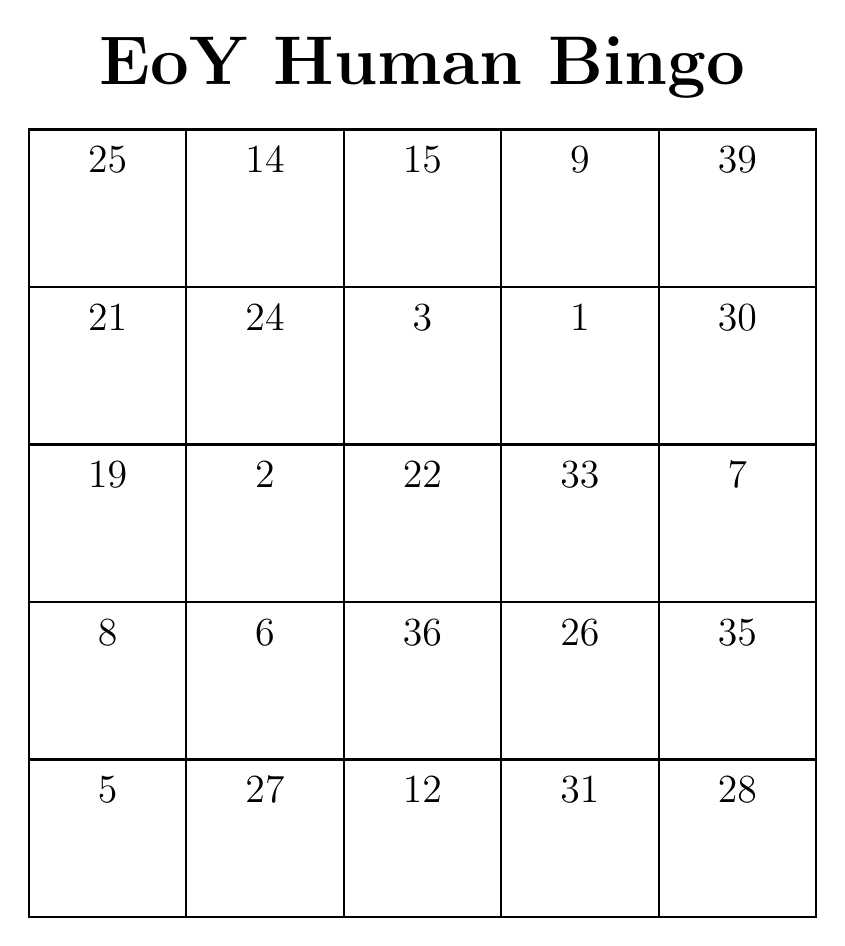
\begin{tikzpicture}
% Set the grid dimensions
\def\cellsize{2cm} % Each cell will be 2x2 cm

% Draw the grid and insert the numbers
\draw[thick] (0, 0) rectangle +(2, 2);
\node[anchor=north, font=\Large, align=center] at (1.0, 1.9) {25};
\draw[thick] (2, 0) rectangle +(2, 2);
\node[anchor=north, font=\Large, align=center] at (3.0, 1.9) {14};
\draw[thick] (4, 0) rectangle +(2, 2);
\node[anchor=north, font=\Large, align=center] at (5.0, 1.9) {15};
\draw[thick] (6, 0) rectangle +(2, 2);
\node[anchor=north, font=\Large, align=center] at (7.0, 1.9) {9};
\draw[thick] (8, 0) rectangle +(2, 2);
\node[anchor=north, font=\Large, align=center] at (9.0, 1.9) {39};
\draw[thick] (0, -2) rectangle +(2, 2);
\node[anchor=north, font=\Large, align=center] at (1.0, -0.1) {21};
\draw[thick] (2, -2) rectangle +(2, 2);
\node[anchor=north, font=\Large, align=center] at (3.0, -0.1) {24};
\draw[thick] (4, -2) rectangle +(2, 2);
\node[anchor=north, font=\Large, align=center] at (5.0, -0.1) {3};
\draw[thick] (6, -2) rectangle +(2, 2);
\node[anchor=north, font=\Large, align=center] at (7.0, -0.1) {1};
\draw[thick] (8, -2) rectangle +(2, 2);
\node[anchor=north, font=\Large, align=center] at (9.0, -0.1) {30};
\draw[thick] (0, -4) rectangle +(2, 2);
\node[anchor=north, font=\Large, align=center] at (1.0, -2.1) {19};
\draw[thick] (2, -4) rectangle +(2, 2);
\node[anchor=north, font=\Large, align=center] at (3.0, -2.1) {2};
\draw[thick] (4, -4) rectangle +(2, 2);
\node[anchor=north, font=\Large, align=center] at (5.0, -2.1) {22};
\draw[thick] (6, -4) rectangle +(2, 2);
\node[anchor=north, font=\Large, align=center] at (7.0, -2.1) {33};
\draw[thick] (8, -4) rectangle +(2, 2);
\node[anchor=north, font=\Large, align=center] at (9.0, -2.1) {7};
\draw[thick] (0, -6) rectangle +(2, 2);
\node[anchor=north, font=\Large, align=center] at (1.0, -4.1) {8};
\draw[thick] (2, -6) rectangle +(2, 2);
\node[anchor=north, font=\Large, align=center] at (3.0, -4.1) {6};
\draw[thick] (4, -6) rectangle +(2, 2);
\node[anchor=north, font=\Large, align=center] at (5.0, -4.1) {36};
\draw[thick] (6, -6) rectangle +(2, 2);
\node[anchor=north, font=\Large, align=center] at (7.0, -4.1) {26};
\draw[thick] (8, -6) rectangle +(2, 2);
\node[anchor=north, font=\Large, align=center] at (9.0, -4.1) {35};
\draw[thick] (0, -8) rectangle +(2, 2);
\node[anchor=north, font=\Large, align=center] at (1.0, -6.1) {5};
\draw[thick] (2, -8) rectangle +(2, 2);
\node[anchor=north, font=\Large, align=center] at (3.0, -6.1) {27};
\draw[thick] (4, -8) rectangle +(2, 2);
\node[anchor=north, font=\Large, align=center] at (5.0, -6.1) {12};
\draw[thick] (6, -8) rectangle +(2, 2);
\node[anchor=north, font=\Large, align=center] at (7.0, -6.1) {31};
\draw[thick] (8, -8) rectangle +(2, 2);
\node[anchor=north, font=\Large, align=center] at (9.0, -6.1) {28};
\node[anchor=north, font = \Huge] at (5.0, 3.3){\textbf{EoY Human Bingo}};
\end{tikzpicture}
\end{center}
\newpage\begin{center}
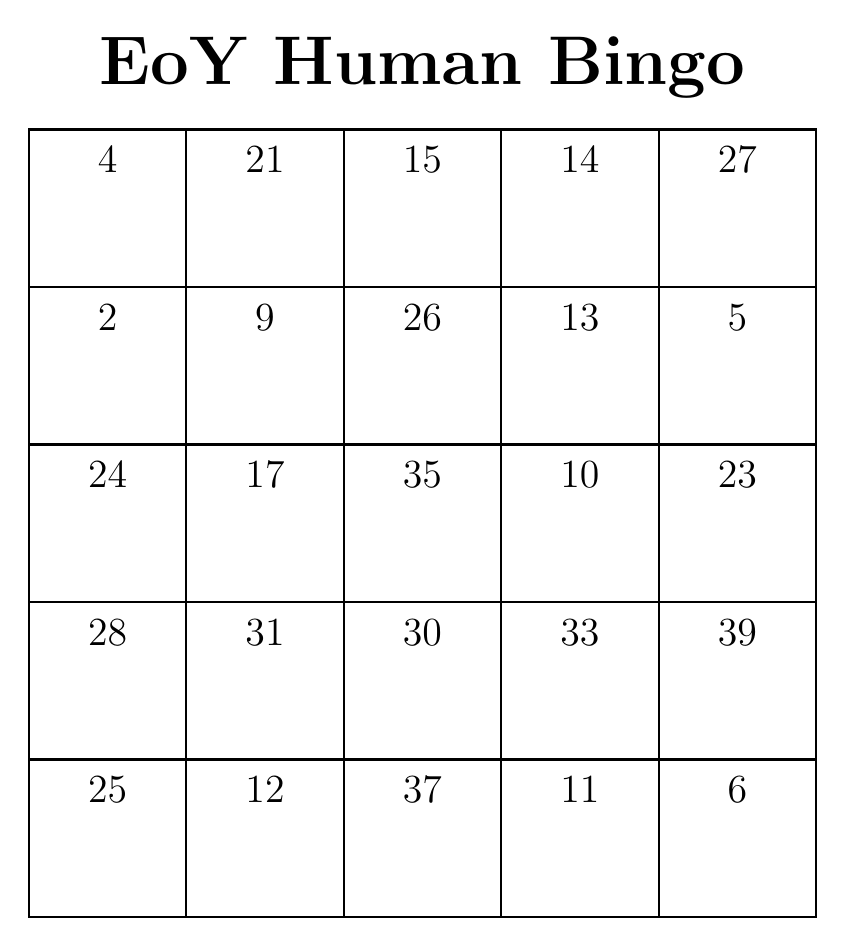
\begin{tikzpicture}
% Set the grid dimensions
\def\cellsize{2cm} % Each cell will be 2x2 cm

% Draw the grid and insert the numbers
\draw[thick] (0, 0) rectangle +(2, 2);
\node[anchor=north, font=\Large, align=center] at (1.0, 1.9) {4};
\draw[thick] (2, 0) rectangle +(2, 2);
\node[anchor=north, font=\Large, align=center] at (3.0, 1.9) {21};
\draw[thick] (4, 0) rectangle +(2, 2);
\node[anchor=north, font=\Large, align=center] at (5.0, 1.9) {15};
\draw[thick] (6, 0) rectangle +(2, 2);
\node[anchor=north, font=\Large, align=center] at (7.0, 1.9) {14};
\draw[thick] (8, 0) rectangle +(2, 2);
\node[anchor=north, font=\Large, align=center] at (9.0, 1.9) {27};
\draw[thick] (0, -2) rectangle +(2, 2);
\node[anchor=north, font=\Large, align=center] at (1.0, -0.1) {2};
\draw[thick] (2, -2) rectangle +(2, 2);
\node[anchor=north, font=\Large, align=center] at (3.0, -0.1) {9};
\draw[thick] (4, -2) rectangle +(2, 2);
\node[anchor=north, font=\Large, align=center] at (5.0, -0.1) {26};
\draw[thick] (6, -2) rectangle +(2, 2);
\node[anchor=north, font=\Large, align=center] at (7.0, -0.1) {13};
\draw[thick] (8, -2) rectangle +(2, 2);
\node[anchor=north, font=\Large, align=center] at (9.0, -0.1) {5};
\draw[thick] (0, -4) rectangle +(2, 2);
\node[anchor=north, font=\Large, align=center] at (1.0, -2.1) {24};
\draw[thick] (2, -4) rectangle +(2, 2);
\node[anchor=north, font=\Large, align=center] at (3.0, -2.1) {17};
\draw[thick] (4, -4) rectangle +(2, 2);
\node[anchor=north, font=\Large, align=center] at (5.0, -2.1) {35};
\draw[thick] (6, -4) rectangle +(2, 2);
\node[anchor=north, font=\Large, align=center] at (7.0, -2.1) {10};
\draw[thick] (8, -4) rectangle +(2, 2);
\node[anchor=north, font=\Large, align=center] at (9.0, -2.1) {23};
\draw[thick] (0, -6) rectangle +(2, 2);
\node[anchor=north, font=\Large, align=center] at (1.0, -4.1) {28};
\draw[thick] (2, -6) rectangle +(2, 2);
\node[anchor=north, font=\Large, align=center] at (3.0, -4.1) {31};
\draw[thick] (4, -6) rectangle +(2, 2);
\node[anchor=north, font=\Large, align=center] at (5.0, -4.1) {30};
\draw[thick] (6, -6) rectangle +(2, 2);
\node[anchor=north, font=\Large, align=center] at (7.0, -4.1) {33};
\draw[thick] (8, -6) rectangle +(2, 2);
\node[anchor=north, font=\Large, align=center] at (9.0, -4.1) {39};
\draw[thick] (0, -8) rectangle +(2, 2);
\node[anchor=north, font=\Large, align=center] at (1.0, -6.1) {25};
\draw[thick] (2, -8) rectangle +(2, 2);
\node[anchor=north, font=\Large, align=center] at (3.0, -6.1) {12};
\draw[thick] (4, -8) rectangle +(2, 2);
\node[anchor=north, font=\Large, align=center] at (5.0, -6.1) {37};
\draw[thick] (6, -8) rectangle +(2, 2);
\node[anchor=north, font=\Large, align=center] at (7.0, -6.1) {11};
\draw[thick] (8, -8) rectangle +(2, 2);
\node[anchor=north, font=\Large, align=center] at (9.0, -6.1) {6};
\node[anchor=north, font = \Huge] at (5.0, 3.3){\textbf{EoY Human Bingo}};
\end{tikzpicture}
\end{center}
\newpage\begin{center}
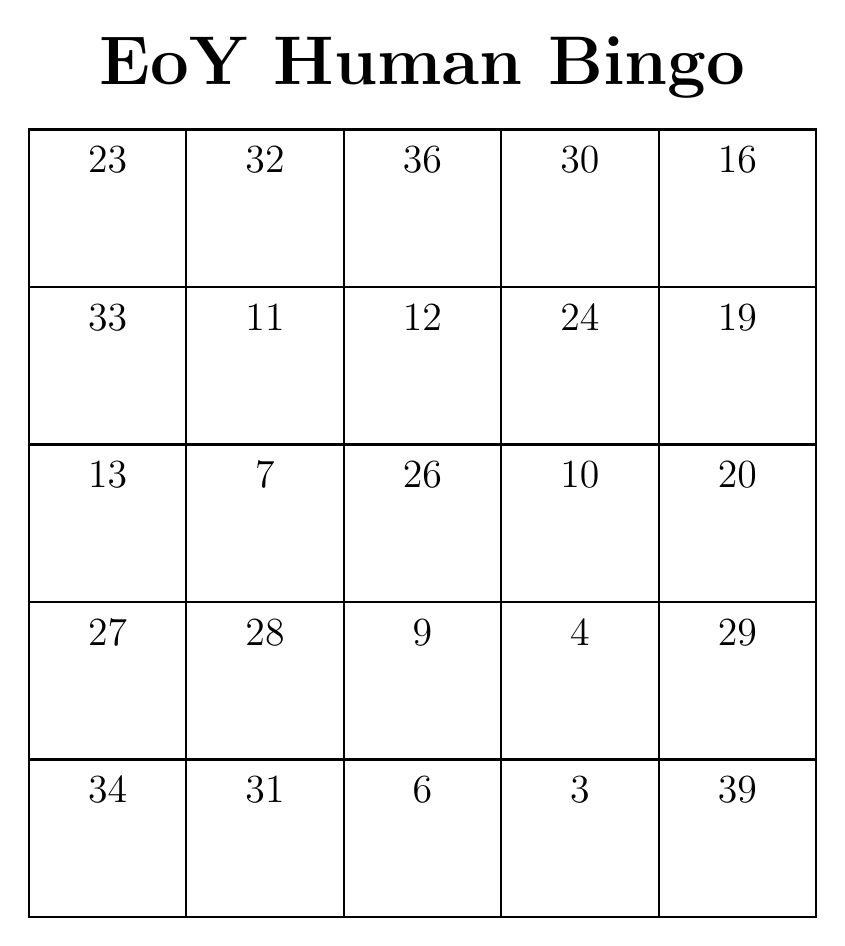
\begin{tikzpicture}
% Set the grid dimensions
\def\cellsize{2cm} % Each cell will be 2x2 cm

% Draw the grid and insert the numbers
\draw[thick] (0, 0) rectangle +(2, 2);
\node[anchor=north, font=\Large, align=center] at (1.0, 1.9) {23};
\draw[thick] (2, 0) rectangle +(2, 2);
\node[anchor=north, font=\Large, align=center] at (3.0, 1.9) {32};
\draw[thick] (4, 0) rectangle +(2, 2);
\node[anchor=north, font=\Large, align=center] at (5.0, 1.9) {36};
\draw[thick] (6, 0) rectangle +(2, 2);
\node[anchor=north, font=\Large, align=center] at (7.0, 1.9) {30};
\draw[thick] (8, 0) rectangle +(2, 2);
\node[anchor=north, font=\Large, align=center] at (9.0, 1.9) {16};
\draw[thick] (0, -2) rectangle +(2, 2);
\node[anchor=north, font=\Large, align=center] at (1.0, -0.1) {33};
\draw[thick] (2, -2) rectangle +(2, 2);
\node[anchor=north, font=\Large, align=center] at (3.0, -0.1) {11};
\draw[thick] (4, -2) rectangle +(2, 2);
\node[anchor=north, font=\Large, align=center] at (5.0, -0.1) {12};
\draw[thick] (6, -2) rectangle +(2, 2);
\node[anchor=north, font=\Large, align=center] at (7.0, -0.1) {24};
\draw[thick] (8, -2) rectangle +(2, 2);
\node[anchor=north, font=\Large, align=center] at (9.0, -0.1) {19};
\draw[thick] (0, -4) rectangle +(2, 2);
\node[anchor=north, font=\Large, align=center] at (1.0, -2.1) {13};
\draw[thick] (2, -4) rectangle +(2, 2);
\node[anchor=north, font=\Large, align=center] at (3.0, -2.1) {7};
\draw[thick] (4, -4) rectangle +(2, 2);
\node[anchor=north, font=\Large, align=center] at (5.0, -2.1) {26};
\draw[thick] (6, -4) rectangle +(2, 2);
\node[anchor=north, font=\Large, align=center] at (7.0, -2.1) {10};
\draw[thick] (8, -4) rectangle +(2, 2);
\node[anchor=north, font=\Large, align=center] at (9.0, -2.1) {20};
\draw[thick] (0, -6) rectangle +(2, 2);
\node[anchor=north, font=\Large, align=center] at (1.0, -4.1) {27};
\draw[thick] (2, -6) rectangle +(2, 2);
\node[anchor=north, font=\Large, align=center] at (3.0, -4.1) {28};
\draw[thick] (4, -6) rectangle +(2, 2);
\node[anchor=north, font=\Large, align=center] at (5.0, -4.1) {9};
\draw[thick] (6, -6) rectangle +(2, 2);
\node[anchor=north, font=\Large, align=center] at (7.0, -4.1) {4};
\draw[thick] (8, -6) rectangle +(2, 2);
\node[anchor=north, font=\Large, align=center] at (9.0, -4.1) {29};
\draw[thick] (0, -8) rectangle +(2, 2);
\node[anchor=north, font=\Large, align=center] at (1.0, -6.1) {34};
\draw[thick] (2, -8) rectangle +(2, 2);
\node[anchor=north, font=\Large, align=center] at (3.0, -6.1) {31};
\draw[thick] (4, -8) rectangle +(2, 2);
\node[anchor=north, font=\Large, align=center] at (5.0, -6.1) {6};
\draw[thick] (6, -8) rectangle +(2, 2);
\node[anchor=north, font=\Large, align=center] at (7.0, -6.1) {3};
\draw[thick] (8, -8) rectangle +(2, 2);
\node[anchor=north, font=\Large, align=center] at (9.0, -6.1) {39};
\node[anchor=north, font = \Huge] at (5.0, 3.3){\textbf{EoY Human Bingo}};
\end{tikzpicture}
\end{center}
\newpage\begin{center}
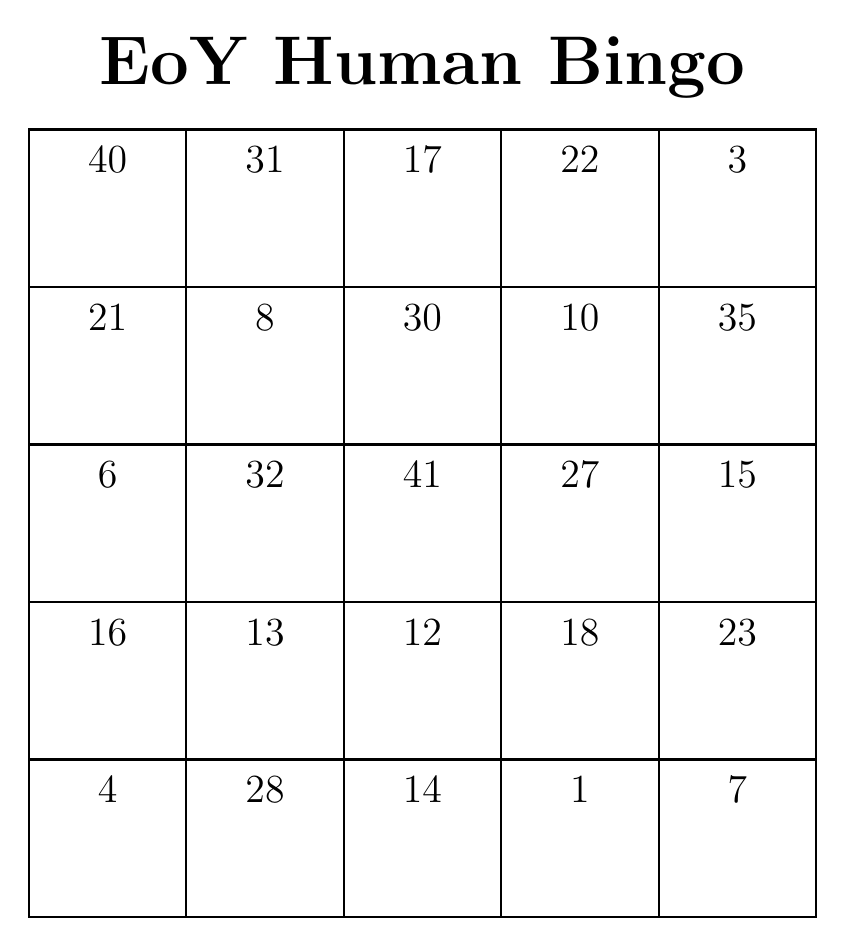
\begin{tikzpicture}
% Set the grid dimensions
\def\cellsize{2cm} % Each cell will be 2x2 cm

% Draw the grid and insert the numbers
\draw[thick] (0, 0) rectangle +(2, 2);
\node[anchor=north, font=\Large, align=center] at (1.0, 1.9) {40};
\draw[thick] (2, 0) rectangle +(2, 2);
\node[anchor=north, font=\Large, align=center] at (3.0, 1.9) {31};
\draw[thick] (4, 0) rectangle +(2, 2);
\node[anchor=north, font=\Large, align=center] at (5.0, 1.9) {17};
\draw[thick] (6, 0) rectangle +(2, 2);
\node[anchor=north, font=\Large, align=center] at (7.0, 1.9) {22};
\draw[thick] (8, 0) rectangle +(2, 2);
\node[anchor=north, font=\Large, align=center] at (9.0, 1.9) {3};
\draw[thick] (0, -2) rectangle +(2, 2);
\node[anchor=north, font=\Large, align=center] at (1.0, -0.1) {21};
\draw[thick] (2, -2) rectangle +(2, 2);
\node[anchor=north, font=\Large, align=center] at (3.0, -0.1) {8};
\draw[thick] (4, -2) rectangle +(2, 2);
\node[anchor=north, font=\Large, align=center] at (5.0, -0.1) {30};
\draw[thick] (6, -2) rectangle +(2, 2);
\node[anchor=north, font=\Large, align=center] at (7.0, -0.1) {10};
\draw[thick] (8, -2) rectangle +(2, 2);
\node[anchor=north, font=\Large, align=center] at (9.0, -0.1) {35};
\draw[thick] (0, -4) rectangle +(2, 2);
\node[anchor=north, font=\Large, align=center] at (1.0, -2.1) {6};
\draw[thick] (2, -4) rectangle +(2, 2);
\node[anchor=north, font=\Large, align=center] at (3.0, -2.1) {32};
\draw[thick] (4, -4) rectangle +(2, 2);
\node[anchor=north, font=\Large, align=center] at (5.0, -2.1) {41};
\draw[thick] (6, -4) rectangle +(2, 2);
\node[anchor=north, font=\Large, align=center] at (7.0, -2.1) {27};
\draw[thick] (8, -4) rectangle +(2, 2);
\node[anchor=north, font=\Large, align=center] at (9.0, -2.1) {15};
\draw[thick] (0, -6) rectangle +(2, 2);
\node[anchor=north, font=\Large, align=center] at (1.0, -4.1) {16};
\draw[thick] (2, -6) rectangle +(2, 2);
\node[anchor=north, font=\Large, align=center] at (3.0, -4.1) {13};
\draw[thick] (4, -6) rectangle +(2, 2);
\node[anchor=north, font=\Large, align=center] at (5.0, -4.1) {12};
\draw[thick] (6, -6) rectangle +(2, 2);
\node[anchor=north, font=\Large, align=center] at (7.0, -4.1) {18};
\draw[thick] (8, -6) rectangle +(2, 2);
\node[anchor=north, font=\Large, align=center] at (9.0, -4.1) {23};
\draw[thick] (0, -8) rectangle +(2, 2);
\node[anchor=north, font=\Large, align=center] at (1.0, -6.1) {4};
\draw[thick] (2, -8) rectangle +(2, 2);
\node[anchor=north, font=\Large, align=center] at (3.0, -6.1) {28};
\draw[thick] (4, -8) rectangle +(2, 2);
\node[anchor=north, font=\Large, align=center] at (5.0, -6.1) {14};
\draw[thick] (6, -8) rectangle +(2, 2);
\node[anchor=north, font=\Large, align=center] at (7.0, -6.1) {1};
\draw[thick] (8, -8) rectangle +(2, 2);
\node[anchor=north, font=\Large, align=center] at (9.0, -6.1) {7};
\node[anchor=north, font = \Huge] at (5.0, 3.3){\textbf{EoY Human Bingo}};
\end{tikzpicture}
\end{center}
\newpage\begin{center}
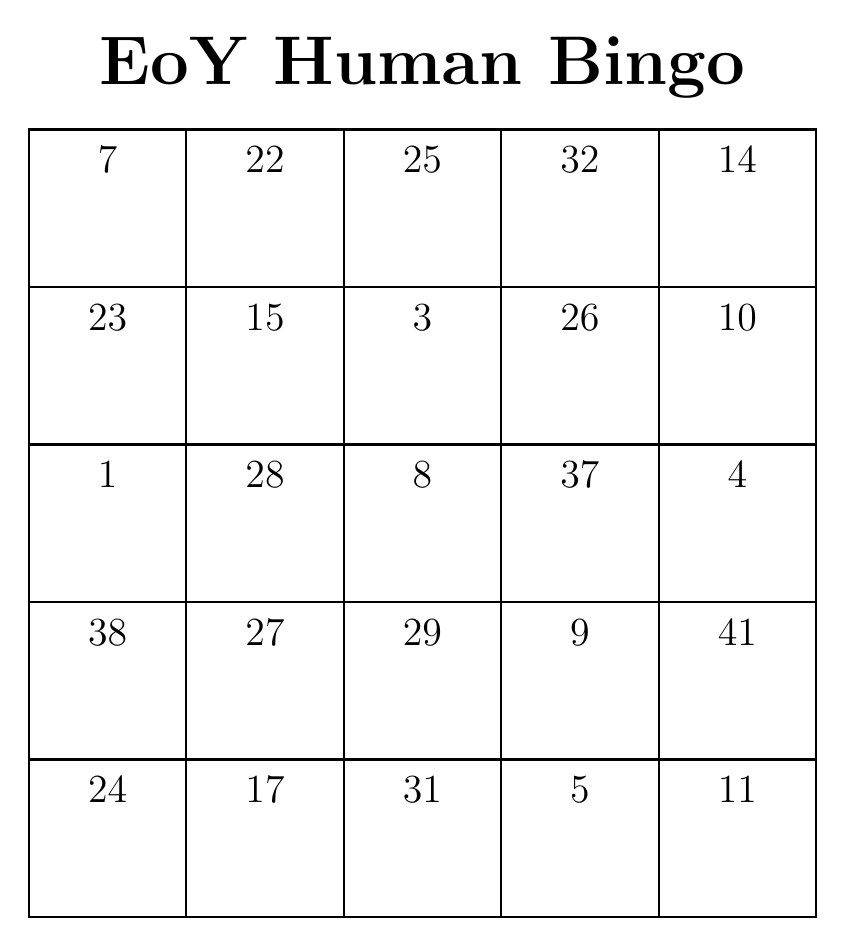
\begin{tikzpicture}
% Set the grid dimensions
\def\cellsize{2cm} % Each cell will be 2x2 cm

% Draw the grid and insert the numbers
\draw[thick] (0, 0) rectangle +(2, 2);
\node[anchor=north, font=\Large, align=center] at (1.0, 1.9) {7};
\draw[thick] (2, 0) rectangle +(2, 2);
\node[anchor=north, font=\Large, align=center] at (3.0, 1.9) {22};
\draw[thick] (4, 0) rectangle +(2, 2);
\node[anchor=north, font=\Large, align=center] at (5.0, 1.9) {25};
\draw[thick] (6, 0) rectangle +(2, 2);
\node[anchor=north, font=\Large, align=center] at (7.0, 1.9) {32};
\draw[thick] (8, 0) rectangle +(2, 2);
\node[anchor=north, font=\Large, align=center] at (9.0, 1.9) {14};
\draw[thick] (0, -2) rectangle +(2, 2);
\node[anchor=north, font=\Large, align=center] at (1.0, -0.1) {23};
\draw[thick] (2, -2) rectangle +(2, 2);
\node[anchor=north, font=\Large, align=center] at (3.0, -0.1) {15};
\draw[thick] (4, -2) rectangle +(2, 2);
\node[anchor=north, font=\Large, align=center] at (5.0, -0.1) {3};
\draw[thick] (6, -2) rectangle +(2, 2);
\node[anchor=north, font=\Large, align=center] at (7.0, -0.1) {26};
\draw[thick] (8, -2) rectangle +(2, 2);
\node[anchor=north, font=\Large, align=center] at (9.0, -0.1) {10};
\draw[thick] (0, -4) rectangle +(2, 2);
\node[anchor=north, font=\Large, align=center] at (1.0, -2.1) {1};
\draw[thick] (2, -4) rectangle +(2, 2);
\node[anchor=north, font=\Large, align=center] at (3.0, -2.1) {28};
\draw[thick] (4, -4) rectangle +(2, 2);
\node[anchor=north, font=\Large, align=center] at (5.0, -2.1) {8};
\draw[thick] (6, -4) rectangle +(2, 2);
\node[anchor=north, font=\Large, align=center] at (7.0, -2.1) {37};
\draw[thick] (8, -4) rectangle +(2, 2);
\node[anchor=north, font=\Large, align=center] at (9.0, -2.1) {4};
\draw[thick] (0, -6) rectangle +(2, 2);
\node[anchor=north, font=\Large, align=center] at (1.0, -4.1) {38};
\draw[thick] (2, -6) rectangle +(2, 2);
\node[anchor=north, font=\Large, align=center] at (3.0, -4.1) {27};
\draw[thick] (4, -6) rectangle +(2, 2);
\node[anchor=north, font=\Large, align=center] at (5.0, -4.1) {29};
\draw[thick] (6, -6) rectangle +(2, 2);
\node[anchor=north, font=\Large, align=center] at (7.0, -4.1) {9};
\draw[thick] (8, -6) rectangle +(2, 2);
\node[anchor=north, font=\Large, align=center] at (9.0, -4.1) {41};
\draw[thick] (0, -8) rectangle +(2, 2);
\node[anchor=north, font=\Large, align=center] at (1.0, -6.1) {24};
\draw[thick] (2, -8) rectangle +(2, 2);
\node[anchor=north, font=\Large, align=center] at (3.0, -6.1) {17};
\draw[thick] (4, -8) rectangle +(2, 2);
\node[anchor=north, font=\Large, align=center] at (5.0, -6.1) {31};
\draw[thick] (6, -8) rectangle +(2, 2);
\node[anchor=north, font=\Large, align=center] at (7.0, -6.1) {5};
\draw[thick] (8, -8) rectangle +(2, 2);
\node[anchor=north, font=\Large, align=center] at (9.0, -6.1) {11};
\node[anchor=north, font = \Huge] at (5.0, 3.3){\textbf{EoY Human Bingo}};
\end{tikzpicture}
\end{center}
\newpage\begin{center}
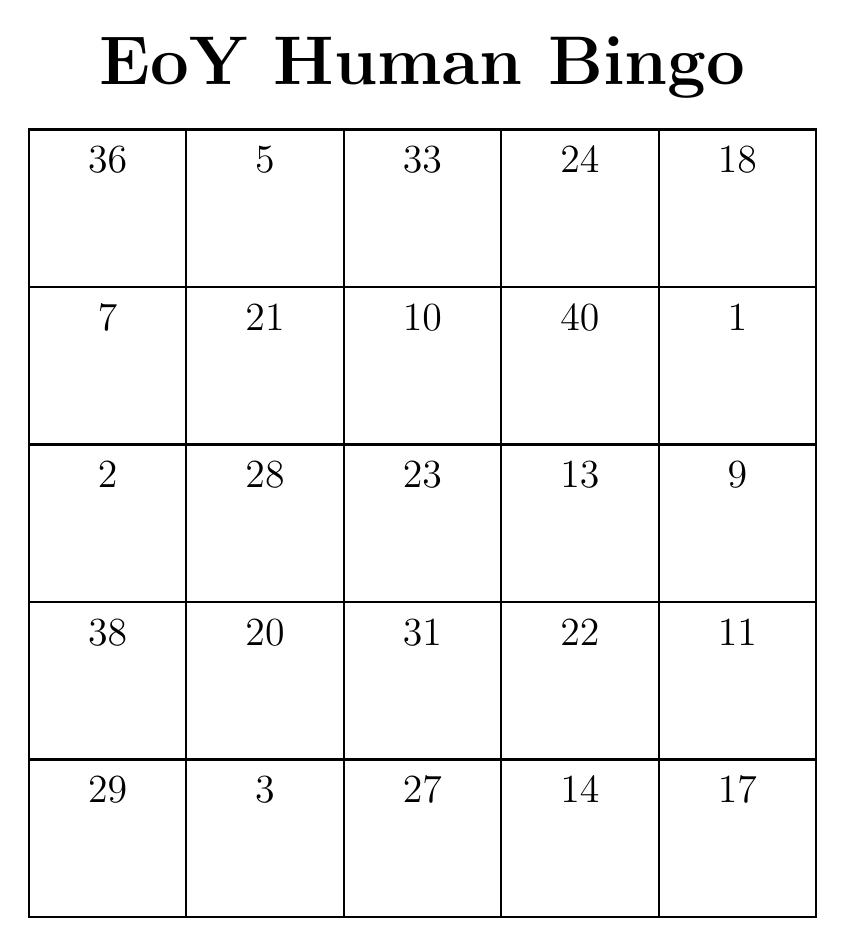
\begin{tikzpicture}
% Set the grid dimensions
\def\cellsize{2cm} % Each cell will be 2x2 cm

% Draw the grid and insert the numbers
\draw[thick] (0, 0) rectangle +(2, 2);
\node[anchor=north, font=\Large, align=center] at (1.0, 1.9) {36};
\draw[thick] (2, 0) rectangle +(2, 2);
\node[anchor=north, font=\Large, align=center] at (3.0, 1.9) {5};
\draw[thick] (4, 0) rectangle +(2, 2);
\node[anchor=north, font=\Large, align=center] at (5.0, 1.9) {33};
\draw[thick] (6, 0) rectangle +(2, 2);
\node[anchor=north, font=\Large, align=center] at (7.0, 1.9) {24};
\draw[thick] (8, 0) rectangle +(2, 2);
\node[anchor=north, font=\Large, align=center] at (9.0, 1.9) {18};
\draw[thick] (0, -2) rectangle +(2, 2);
\node[anchor=north, font=\Large, align=center] at (1.0, -0.1) {7};
\draw[thick] (2, -2) rectangle +(2, 2);
\node[anchor=north, font=\Large, align=center] at (3.0, -0.1) {21};
\draw[thick] (4, -2) rectangle +(2, 2);
\node[anchor=north, font=\Large, align=center] at (5.0, -0.1) {10};
\draw[thick] (6, -2) rectangle +(2, 2);
\node[anchor=north, font=\Large, align=center] at (7.0, -0.1) {40};
\draw[thick] (8, -2) rectangle +(2, 2);
\node[anchor=north, font=\Large, align=center] at (9.0, -0.1) {1};
\draw[thick] (0, -4) rectangle +(2, 2);
\node[anchor=north, font=\Large, align=center] at (1.0, -2.1) {2};
\draw[thick] (2, -4) rectangle +(2, 2);
\node[anchor=north, font=\Large, align=center] at (3.0, -2.1) {28};
\draw[thick] (4, -4) rectangle +(2, 2);
\node[anchor=north, font=\Large, align=center] at (5.0, -2.1) {23};
\draw[thick] (6, -4) rectangle +(2, 2);
\node[anchor=north, font=\Large, align=center] at (7.0, -2.1) {13};
\draw[thick] (8, -4) rectangle +(2, 2);
\node[anchor=north, font=\Large, align=center] at (9.0, -2.1) {9};
\draw[thick] (0, -6) rectangle +(2, 2);
\node[anchor=north, font=\Large, align=center] at (1.0, -4.1) {38};
\draw[thick] (2, -6) rectangle +(2, 2);
\node[anchor=north, font=\Large, align=center] at (3.0, -4.1) {20};
\draw[thick] (4, -6) rectangle +(2, 2);
\node[anchor=north, font=\Large, align=center] at (5.0, -4.1) {31};
\draw[thick] (6, -6) rectangle +(2, 2);
\node[anchor=north, font=\Large, align=center] at (7.0, -4.1) {22};
\draw[thick] (8, -6) rectangle +(2, 2);
\node[anchor=north, font=\Large, align=center] at (9.0, -4.1) {11};
\draw[thick] (0, -8) rectangle +(2, 2);
\node[anchor=north, font=\Large, align=center] at (1.0, -6.1) {29};
\draw[thick] (2, -8) rectangle +(2, 2);
\node[anchor=north, font=\Large, align=center] at (3.0, -6.1) {3};
\draw[thick] (4, -8) rectangle +(2, 2);
\node[anchor=north, font=\Large, align=center] at (5.0, -6.1) {27};
\draw[thick] (6, -8) rectangle +(2, 2);
\node[anchor=north, font=\Large, align=center] at (7.0, -6.1) {14};
\draw[thick] (8, -8) rectangle +(2, 2);
\node[anchor=north, font=\Large, align=center] at (9.0, -6.1) {17};
\node[anchor=north, font = \Huge] at (5.0, 3.3){\textbf{EoY Human Bingo}};
\end{tikzpicture}
\end{center}
\newpage\begin{center}
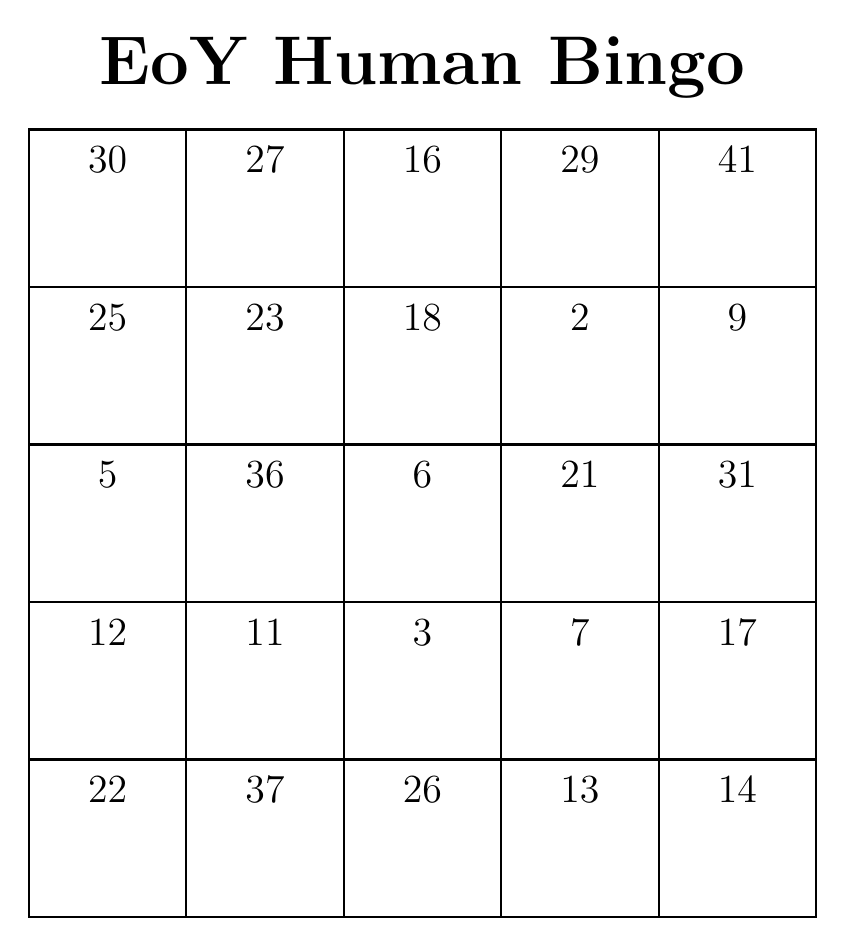
\begin{tikzpicture}
% Set the grid dimensions
\def\cellsize{2cm} % Each cell will be 2x2 cm

% Draw the grid and insert the numbers
\draw[thick] (0, 0) rectangle +(2, 2);
\node[anchor=north, font=\Large, align=center] at (1.0, 1.9) {30};
\draw[thick] (2, 0) rectangle +(2, 2);
\node[anchor=north, font=\Large, align=center] at (3.0, 1.9) {27};
\draw[thick] (4, 0) rectangle +(2, 2);
\node[anchor=north, font=\Large, align=center] at (5.0, 1.9) {16};
\draw[thick] (6, 0) rectangle +(2, 2);
\node[anchor=north, font=\Large, align=center] at (7.0, 1.9) {29};
\draw[thick] (8, 0) rectangle +(2, 2);
\node[anchor=north, font=\Large, align=center] at (9.0, 1.9) {41};
\draw[thick] (0, -2) rectangle +(2, 2);
\node[anchor=north, font=\Large, align=center] at (1.0, -0.1) {25};
\draw[thick] (2, -2) rectangle +(2, 2);
\node[anchor=north, font=\Large, align=center] at (3.0, -0.1) {23};
\draw[thick] (4, -2) rectangle +(2, 2);
\node[anchor=north, font=\Large, align=center] at (5.0, -0.1) {18};
\draw[thick] (6, -2) rectangle +(2, 2);
\node[anchor=north, font=\Large, align=center] at (7.0, -0.1) {2};
\draw[thick] (8, -2) rectangle +(2, 2);
\node[anchor=north, font=\Large, align=center] at (9.0, -0.1) {9};
\draw[thick] (0, -4) rectangle +(2, 2);
\node[anchor=north, font=\Large, align=center] at (1.0, -2.1) {5};
\draw[thick] (2, -4) rectangle +(2, 2);
\node[anchor=north, font=\Large, align=center] at (3.0, -2.1) {36};
\draw[thick] (4, -4) rectangle +(2, 2);
\node[anchor=north, font=\Large, align=center] at (5.0, -2.1) {6};
\draw[thick] (6, -4) rectangle +(2, 2);
\node[anchor=north, font=\Large, align=center] at (7.0, -2.1) {21};
\draw[thick] (8, -4) rectangle +(2, 2);
\node[anchor=north, font=\Large, align=center] at (9.0, -2.1) {31};
\draw[thick] (0, -6) rectangle +(2, 2);
\node[anchor=north, font=\Large, align=center] at (1.0, -4.1) {12};
\draw[thick] (2, -6) rectangle +(2, 2);
\node[anchor=north, font=\Large, align=center] at (3.0, -4.1) {11};
\draw[thick] (4, -6) rectangle +(2, 2);
\node[anchor=north, font=\Large, align=center] at (5.0, -4.1) {3};
\draw[thick] (6, -6) rectangle +(2, 2);
\node[anchor=north, font=\Large, align=center] at (7.0, -4.1) {7};
\draw[thick] (8, -6) rectangle +(2, 2);
\node[anchor=north, font=\Large, align=center] at (9.0, -4.1) {17};
\draw[thick] (0, -8) rectangle +(2, 2);
\node[anchor=north, font=\Large, align=center] at (1.0, -6.1) {22};
\draw[thick] (2, -8) rectangle +(2, 2);
\node[anchor=north, font=\Large, align=center] at (3.0, -6.1) {37};
\draw[thick] (4, -8) rectangle +(2, 2);
\node[anchor=north, font=\Large, align=center] at (5.0, -6.1) {26};
\draw[thick] (6, -8) rectangle +(2, 2);
\node[anchor=north, font=\Large, align=center] at (7.0, -6.1) {13};
\draw[thick] (8, -8) rectangle +(2, 2);
\node[anchor=north, font=\Large, align=center] at (9.0, -6.1) {14};
\node[anchor=north, font = \Huge] at (5.0, 3.3){\textbf{EoY Human Bingo}};
\end{tikzpicture}
\end{center}
\newpage\begin{center}
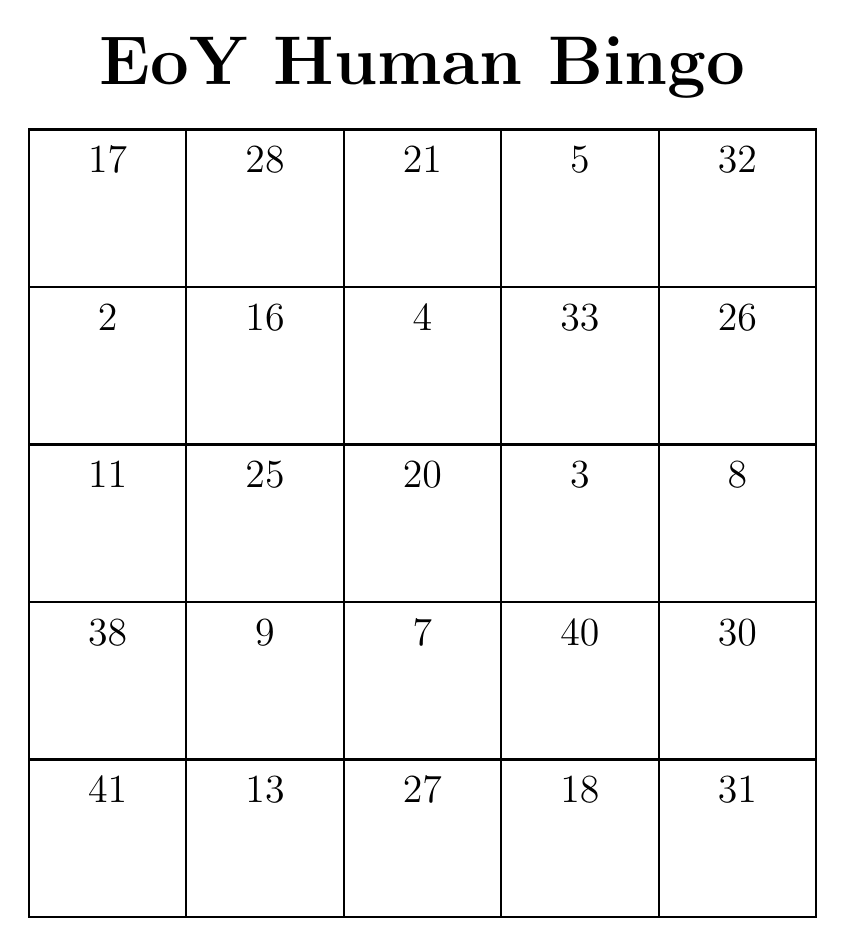
\begin{tikzpicture}
% Set the grid dimensions
\def\cellsize{2cm} % Each cell will be 2x2 cm

% Draw the grid and insert the numbers
\draw[thick] (0, 0) rectangle +(2, 2);
\node[anchor=north, font=\Large, align=center] at (1.0, 1.9) {17};
\draw[thick] (2, 0) rectangle +(2, 2);
\node[anchor=north, font=\Large, align=center] at (3.0, 1.9) {28};
\draw[thick] (4, 0) rectangle +(2, 2);
\node[anchor=north, font=\Large, align=center] at (5.0, 1.9) {21};
\draw[thick] (6, 0) rectangle +(2, 2);
\node[anchor=north, font=\Large, align=center] at (7.0, 1.9) {5};
\draw[thick] (8, 0) rectangle +(2, 2);
\node[anchor=north, font=\Large, align=center] at (9.0, 1.9) {32};
\draw[thick] (0, -2) rectangle +(2, 2);
\node[anchor=north, font=\Large, align=center] at (1.0, -0.1) {2};
\draw[thick] (2, -2) rectangle +(2, 2);
\node[anchor=north, font=\Large, align=center] at (3.0, -0.1) {16};
\draw[thick] (4, -2) rectangle +(2, 2);
\node[anchor=north, font=\Large, align=center] at (5.0, -0.1) {4};
\draw[thick] (6, -2) rectangle +(2, 2);
\node[anchor=north, font=\Large, align=center] at (7.0, -0.1) {33};
\draw[thick] (8, -2) rectangle +(2, 2);
\node[anchor=north, font=\Large, align=center] at (9.0, -0.1) {26};
\draw[thick] (0, -4) rectangle +(2, 2);
\node[anchor=north, font=\Large, align=center] at (1.0, -2.1) {11};
\draw[thick] (2, -4) rectangle +(2, 2);
\node[anchor=north, font=\Large, align=center] at (3.0, -2.1) {25};
\draw[thick] (4, -4) rectangle +(2, 2);
\node[anchor=north, font=\Large, align=center] at (5.0, -2.1) {20};
\draw[thick] (6, -4) rectangle +(2, 2);
\node[anchor=north, font=\Large, align=center] at (7.0, -2.1) {3};
\draw[thick] (8, -4) rectangle +(2, 2);
\node[anchor=north, font=\Large, align=center] at (9.0, -2.1) {8};
\draw[thick] (0, -6) rectangle +(2, 2);
\node[anchor=north, font=\Large, align=center] at (1.0, -4.1) {38};
\draw[thick] (2, -6) rectangle +(2, 2);
\node[anchor=north, font=\Large, align=center] at (3.0, -4.1) {9};
\draw[thick] (4, -6) rectangle +(2, 2);
\node[anchor=north, font=\Large, align=center] at (5.0, -4.1) {7};
\draw[thick] (6, -6) rectangle +(2, 2);
\node[anchor=north, font=\Large, align=center] at (7.0, -4.1) {40};
\draw[thick] (8, -6) rectangle +(2, 2);
\node[anchor=north, font=\Large, align=center] at (9.0, -4.1) {30};
\draw[thick] (0, -8) rectangle +(2, 2);
\node[anchor=north, font=\Large, align=center] at (1.0, -6.1) {41};
\draw[thick] (2, -8) rectangle +(2, 2);
\node[anchor=north, font=\Large, align=center] at (3.0, -6.1) {13};
\draw[thick] (4, -8) rectangle +(2, 2);
\node[anchor=north, font=\Large, align=center] at (5.0, -6.1) {27};
\draw[thick] (6, -8) rectangle +(2, 2);
\node[anchor=north, font=\Large, align=center] at (7.0, -6.1) {18};
\draw[thick] (8, -8) rectangle +(2, 2);
\node[anchor=north, font=\Large, align=center] at (9.0, -6.1) {31};
\node[anchor=north, font = \Huge] at (5.0, 3.3){\textbf{EoY Human Bingo}};
\end{tikzpicture}
\end{center}
\newpage\begin{center}
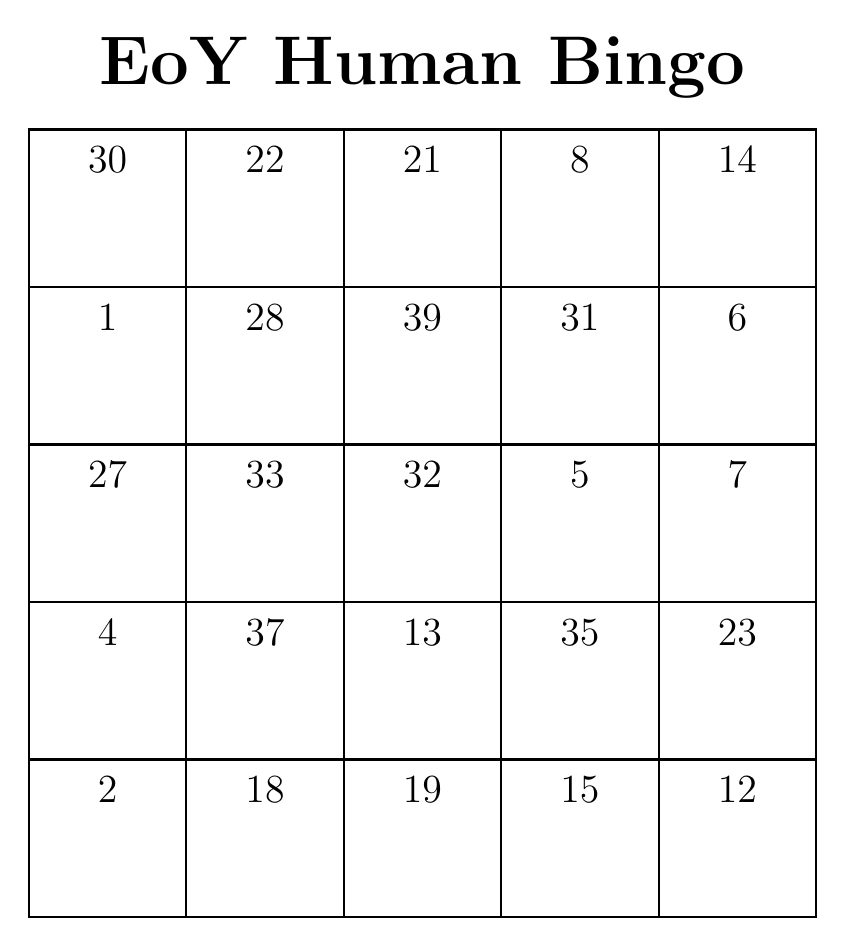
\begin{tikzpicture}
% Set the grid dimensions
\def\cellsize{2cm} % Each cell will be 2x2 cm

% Draw the grid and insert the numbers
\draw[thick] (0, 0) rectangle +(2, 2);
\node[anchor=north, font=\Large, align=center] at (1.0, 1.9) {30};
\draw[thick] (2, 0) rectangle +(2, 2);
\node[anchor=north, font=\Large, align=center] at (3.0, 1.9) {22};
\draw[thick] (4, 0) rectangle +(2, 2);
\node[anchor=north, font=\Large, align=center] at (5.0, 1.9) {21};
\draw[thick] (6, 0) rectangle +(2, 2);
\node[anchor=north, font=\Large, align=center] at (7.0, 1.9) {8};
\draw[thick] (8, 0) rectangle +(2, 2);
\node[anchor=north, font=\Large, align=center] at (9.0, 1.9) {14};
\draw[thick] (0, -2) rectangle +(2, 2);
\node[anchor=north, font=\Large, align=center] at (1.0, -0.1) {1};
\draw[thick] (2, -2) rectangle +(2, 2);
\node[anchor=north, font=\Large, align=center] at (3.0, -0.1) {28};
\draw[thick] (4, -2) rectangle +(2, 2);
\node[anchor=north, font=\Large, align=center] at (5.0, -0.1) {39};
\draw[thick] (6, -2) rectangle +(2, 2);
\node[anchor=north, font=\Large, align=center] at (7.0, -0.1) {31};
\draw[thick] (8, -2) rectangle +(2, 2);
\node[anchor=north, font=\Large, align=center] at (9.0, -0.1) {6};
\draw[thick] (0, -4) rectangle +(2, 2);
\node[anchor=north, font=\Large, align=center] at (1.0, -2.1) {27};
\draw[thick] (2, -4) rectangle +(2, 2);
\node[anchor=north, font=\Large, align=center] at (3.0, -2.1) {33};
\draw[thick] (4, -4) rectangle +(2, 2);
\node[anchor=north, font=\Large, align=center] at (5.0, -2.1) {32};
\draw[thick] (6, -4) rectangle +(2, 2);
\node[anchor=north, font=\Large, align=center] at (7.0, -2.1) {5};
\draw[thick] (8, -4) rectangle +(2, 2);
\node[anchor=north, font=\Large, align=center] at (9.0, -2.1) {7};
\draw[thick] (0, -6) rectangle +(2, 2);
\node[anchor=north, font=\Large, align=center] at (1.0, -4.1) {4};
\draw[thick] (2, -6) rectangle +(2, 2);
\node[anchor=north, font=\Large, align=center] at (3.0, -4.1) {37};
\draw[thick] (4, -6) rectangle +(2, 2);
\node[anchor=north, font=\Large, align=center] at (5.0, -4.1) {13};
\draw[thick] (6, -6) rectangle +(2, 2);
\node[anchor=north, font=\Large, align=center] at (7.0, -4.1) {35};
\draw[thick] (8, -6) rectangle +(2, 2);
\node[anchor=north, font=\Large, align=center] at (9.0, -4.1) {23};
\draw[thick] (0, -8) rectangle +(2, 2);
\node[anchor=north, font=\Large, align=center] at (1.0, -6.1) {2};
\draw[thick] (2, -8) rectangle +(2, 2);
\node[anchor=north, font=\Large, align=center] at (3.0, -6.1) {18};
\draw[thick] (4, -8) rectangle +(2, 2);
\node[anchor=north, font=\Large, align=center] at (5.0, -6.1) {19};
\draw[thick] (6, -8) rectangle +(2, 2);
\node[anchor=north, font=\Large, align=center] at (7.0, -6.1) {15};
\draw[thick] (8, -8) rectangle +(2, 2);
\node[anchor=north, font=\Large, align=center] at (9.0, -6.1) {12};
\node[anchor=north, font = \Huge] at (5.0, 3.3){\textbf{EoY Human Bingo}};
\end{tikzpicture}
\end{center}
\newpage\begin{center}
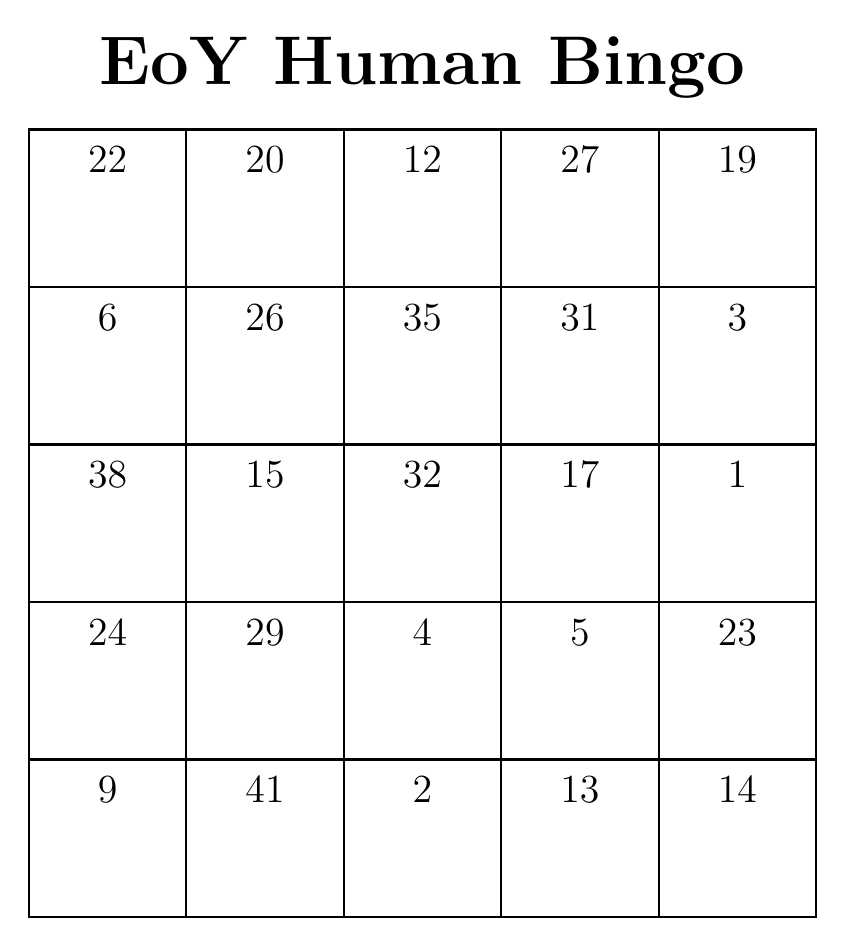
\begin{tikzpicture}
% Set the grid dimensions
\def\cellsize{2cm} % Each cell will be 2x2 cm

% Draw the grid and insert the numbers
\draw[thick] (0, 0) rectangle +(2, 2);
\node[anchor=north, font=\Large, align=center] at (1.0, 1.9) {22};
\draw[thick] (2, 0) rectangle +(2, 2);
\node[anchor=north, font=\Large, align=center] at (3.0, 1.9) {20};
\draw[thick] (4, 0) rectangle +(2, 2);
\node[anchor=north, font=\Large, align=center] at (5.0, 1.9) {12};
\draw[thick] (6, 0) rectangle +(2, 2);
\node[anchor=north, font=\Large, align=center] at (7.0, 1.9) {27};
\draw[thick] (8, 0) rectangle +(2, 2);
\node[anchor=north, font=\Large, align=center] at (9.0, 1.9) {19};
\draw[thick] (0, -2) rectangle +(2, 2);
\node[anchor=north, font=\Large, align=center] at (1.0, -0.1) {6};
\draw[thick] (2, -2) rectangle +(2, 2);
\node[anchor=north, font=\Large, align=center] at (3.0, -0.1) {26};
\draw[thick] (4, -2) rectangle +(2, 2);
\node[anchor=north, font=\Large, align=center] at (5.0, -0.1) {35};
\draw[thick] (6, -2) rectangle +(2, 2);
\node[anchor=north, font=\Large, align=center] at (7.0, -0.1) {31};
\draw[thick] (8, -2) rectangle +(2, 2);
\node[anchor=north, font=\Large, align=center] at (9.0, -0.1) {3};
\draw[thick] (0, -4) rectangle +(2, 2);
\node[anchor=north, font=\Large, align=center] at (1.0, -2.1) {38};
\draw[thick] (2, -4) rectangle +(2, 2);
\node[anchor=north, font=\Large, align=center] at (3.0, -2.1) {15};
\draw[thick] (4, -4) rectangle +(2, 2);
\node[anchor=north, font=\Large, align=center] at (5.0, -2.1) {32};
\draw[thick] (6, -4) rectangle +(2, 2);
\node[anchor=north, font=\Large, align=center] at (7.0, -2.1) {17};
\draw[thick] (8, -4) rectangle +(2, 2);
\node[anchor=north, font=\Large, align=center] at (9.0, -2.1) {1};
\draw[thick] (0, -6) rectangle +(2, 2);
\node[anchor=north, font=\Large, align=center] at (1.0, -4.1) {24};
\draw[thick] (2, -6) rectangle +(2, 2);
\node[anchor=north, font=\Large, align=center] at (3.0, -4.1) {29};
\draw[thick] (4, -6) rectangle +(2, 2);
\node[anchor=north, font=\Large, align=center] at (5.0, -4.1) {4};
\draw[thick] (6, -6) rectangle +(2, 2);
\node[anchor=north, font=\Large, align=center] at (7.0, -4.1) {5};
\draw[thick] (8, -6) rectangle +(2, 2);
\node[anchor=north, font=\Large, align=center] at (9.0, -4.1) {23};
\draw[thick] (0, -8) rectangle +(2, 2);
\node[anchor=north, font=\Large, align=center] at (1.0, -6.1) {9};
\draw[thick] (2, -8) rectangle +(2, 2);
\node[anchor=north, font=\Large, align=center] at (3.0, -6.1) {41};
\draw[thick] (4, -8) rectangle +(2, 2);
\node[anchor=north, font=\Large, align=center] at (5.0, -6.1) {2};
\draw[thick] (6, -8) rectangle +(2, 2);
\node[anchor=north, font=\Large, align=center] at (7.0, -6.1) {13};
\draw[thick] (8, -8) rectangle +(2, 2);
\node[anchor=north, font=\Large, align=center] at (9.0, -6.1) {14};
\node[anchor=north, font = \Huge] at (5.0, 3.3){\textbf{EoY Human Bingo}};
\end{tikzpicture}
\end{center}
\newpage\begin{center}
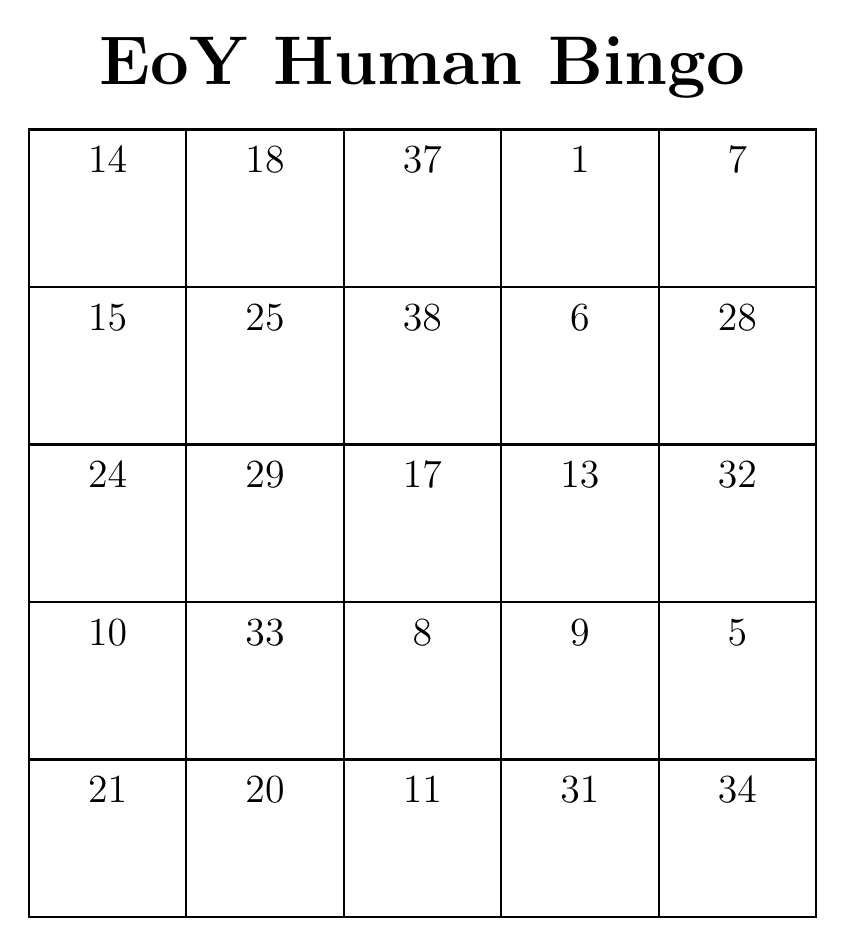
\begin{tikzpicture}
% Set the grid dimensions
\def\cellsize{2cm} % Each cell will be 2x2 cm

% Draw the grid and insert the numbers
\draw[thick] (0, 0) rectangle +(2, 2);
\node[anchor=north, font=\Large, align=center] at (1.0, 1.9) {14};
\draw[thick] (2, 0) rectangle +(2, 2);
\node[anchor=north, font=\Large, align=center] at (3.0, 1.9) {18};
\draw[thick] (4, 0) rectangle +(2, 2);
\node[anchor=north, font=\Large, align=center] at (5.0, 1.9) {37};
\draw[thick] (6, 0) rectangle +(2, 2);
\node[anchor=north, font=\Large, align=center] at (7.0, 1.9) {1};
\draw[thick] (8, 0) rectangle +(2, 2);
\node[anchor=north, font=\Large, align=center] at (9.0, 1.9) {7};
\draw[thick] (0, -2) rectangle +(2, 2);
\node[anchor=north, font=\Large, align=center] at (1.0, -0.1) {15};
\draw[thick] (2, -2) rectangle +(2, 2);
\node[anchor=north, font=\Large, align=center] at (3.0, -0.1) {25};
\draw[thick] (4, -2) rectangle +(2, 2);
\node[anchor=north, font=\Large, align=center] at (5.0, -0.1) {38};
\draw[thick] (6, -2) rectangle +(2, 2);
\node[anchor=north, font=\Large, align=center] at (7.0, -0.1) {6};
\draw[thick] (8, -2) rectangle +(2, 2);
\node[anchor=north, font=\Large, align=center] at (9.0, -0.1) {28};
\draw[thick] (0, -4) rectangle +(2, 2);
\node[anchor=north, font=\Large, align=center] at (1.0, -2.1) {24};
\draw[thick] (2, -4) rectangle +(2, 2);
\node[anchor=north, font=\Large, align=center] at (3.0, -2.1) {29};
\draw[thick] (4, -4) rectangle +(2, 2);
\node[anchor=north, font=\Large, align=center] at (5.0, -2.1) {17};
\draw[thick] (6, -4) rectangle +(2, 2);
\node[anchor=north, font=\Large, align=center] at (7.0, -2.1) {13};
\draw[thick] (8, -4) rectangle +(2, 2);
\node[anchor=north, font=\Large, align=center] at (9.0, -2.1) {32};
\draw[thick] (0, -6) rectangle +(2, 2);
\node[anchor=north, font=\Large, align=center] at (1.0, -4.1) {10};
\draw[thick] (2, -6) rectangle +(2, 2);
\node[anchor=north, font=\Large, align=center] at (3.0, -4.1) {33};
\draw[thick] (4, -6) rectangle +(2, 2);
\node[anchor=north, font=\Large, align=center] at (5.0, -4.1) {8};
\draw[thick] (6, -6) rectangle +(2, 2);
\node[anchor=north, font=\Large, align=center] at (7.0, -4.1) {9};
\draw[thick] (8, -6) rectangle +(2, 2);
\node[anchor=north, font=\Large, align=center] at (9.0, -4.1) {5};
\draw[thick] (0, -8) rectangle +(2, 2);
\node[anchor=north, font=\Large, align=center] at (1.0, -6.1) {21};
\draw[thick] (2, -8) rectangle +(2, 2);
\node[anchor=north, font=\Large, align=center] at (3.0, -6.1) {20};
\draw[thick] (4, -8) rectangle +(2, 2);
\node[anchor=north, font=\Large, align=center] at (5.0, -6.1) {11};
\draw[thick] (6, -8) rectangle +(2, 2);
\node[anchor=north, font=\Large, align=center] at (7.0, -6.1) {31};
\draw[thick] (8, -8) rectangle +(2, 2);
\node[anchor=north, font=\Large, align=center] at (9.0, -6.1) {34};
\node[anchor=north, font = \Huge] at (5.0, 3.3){\textbf{EoY Human Bingo}};
\end{tikzpicture}
\end{center}
\newpage\begin{center}
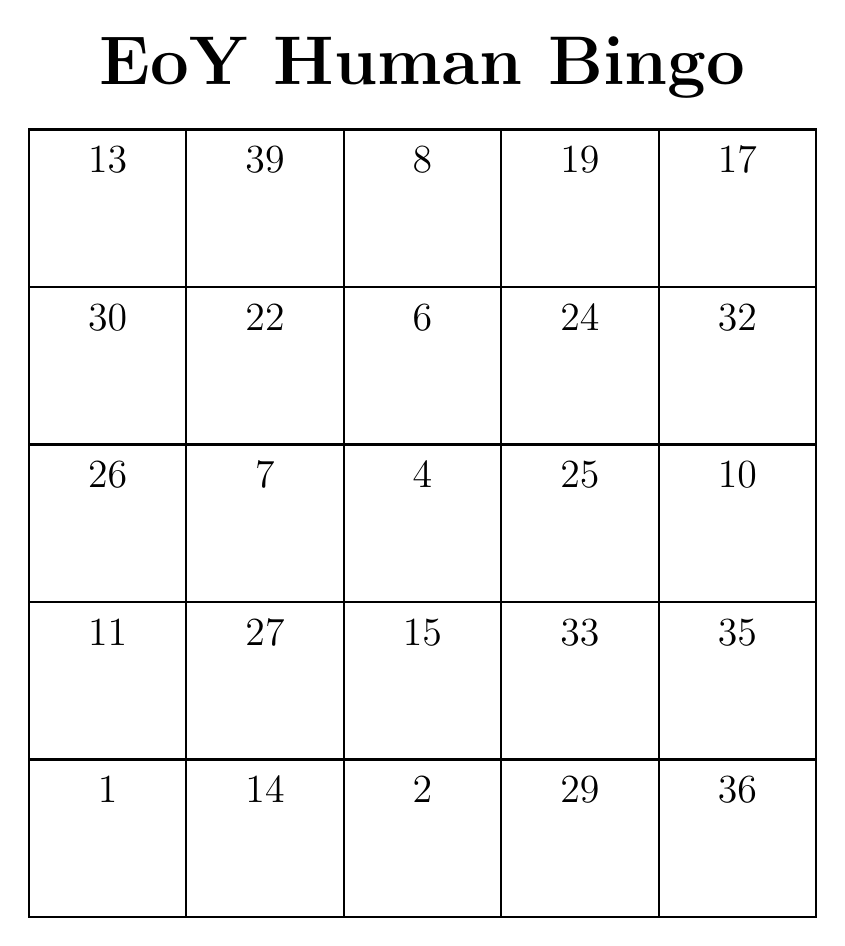
\begin{tikzpicture}
% Set the grid dimensions
\def\cellsize{2cm} % Each cell will be 2x2 cm

% Draw the grid and insert the numbers
\draw[thick] (0, 0) rectangle +(2, 2);
\node[anchor=north, font=\Large, align=center] at (1.0, 1.9) {13};
\draw[thick] (2, 0) rectangle +(2, 2);
\node[anchor=north, font=\Large, align=center] at (3.0, 1.9) {39};
\draw[thick] (4, 0) rectangle +(2, 2);
\node[anchor=north, font=\Large, align=center] at (5.0, 1.9) {8};
\draw[thick] (6, 0) rectangle +(2, 2);
\node[anchor=north, font=\Large, align=center] at (7.0, 1.9) {19};
\draw[thick] (8, 0) rectangle +(2, 2);
\node[anchor=north, font=\Large, align=center] at (9.0, 1.9) {17};
\draw[thick] (0, -2) rectangle +(2, 2);
\node[anchor=north, font=\Large, align=center] at (1.0, -0.1) {30};
\draw[thick] (2, -2) rectangle +(2, 2);
\node[anchor=north, font=\Large, align=center] at (3.0, -0.1) {22};
\draw[thick] (4, -2) rectangle +(2, 2);
\node[anchor=north, font=\Large, align=center] at (5.0, -0.1) {6};
\draw[thick] (6, -2) rectangle +(2, 2);
\node[anchor=north, font=\Large, align=center] at (7.0, -0.1) {24};
\draw[thick] (8, -2) rectangle +(2, 2);
\node[anchor=north, font=\Large, align=center] at (9.0, -0.1) {32};
\draw[thick] (0, -4) rectangle +(2, 2);
\node[anchor=north, font=\Large, align=center] at (1.0, -2.1) {26};
\draw[thick] (2, -4) rectangle +(2, 2);
\node[anchor=north, font=\Large, align=center] at (3.0, -2.1) {7};
\draw[thick] (4, -4) rectangle +(2, 2);
\node[anchor=north, font=\Large, align=center] at (5.0, -2.1) {4};
\draw[thick] (6, -4) rectangle +(2, 2);
\node[anchor=north, font=\Large, align=center] at (7.0, -2.1) {25};
\draw[thick] (8, -4) rectangle +(2, 2);
\node[anchor=north, font=\Large, align=center] at (9.0, -2.1) {10};
\draw[thick] (0, -6) rectangle +(2, 2);
\node[anchor=north, font=\Large, align=center] at (1.0, -4.1) {11};
\draw[thick] (2, -6) rectangle +(2, 2);
\node[anchor=north, font=\Large, align=center] at (3.0, -4.1) {27};
\draw[thick] (4, -6) rectangle +(2, 2);
\node[anchor=north, font=\Large, align=center] at (5.0, -4.1) {15};
\draw[thick] (6, -6) rectangle +(2, 2);
\node[anchor=north, font=\Large, align=center] at (7.0, -4.1) {33};
\draw[thick] (8, -6) rectangle +(2, 2);
\node[anchor=north, font=\Large, align=center] at (9.0, -4.1) {35};
\draw[thick] (0, -8) rectangle +(2, 2);
\node[anchor=north, font=\Large, align=center] at (1.0, -6.1) {1};
\draw[thick] (2, -8) rectangle +(2, 2);
\node[anchor=north, font=\Large, align=center] at (3.0, -6.1) {14};
\draw[thick] (4, -8) rectangle +(2, 2);
\node[anchor=north, font=\Large, align=center] at (5.0, -6.1) {2};
\draw[thick] (6, -8) rectangle +(2, 2);
\node[anchor=north, font=\Large, align=center] at (7.0, -6.1) {29};
\draw[thick] (8, -8) rectangle +(2, 2);
\node[anchor=north, font=\Large, align=center] at (9.0, -6.1) {36};
\node[anchor=north, font = \Huge] at (5.0, 3.3){\textbf{EoY Human Bingo}};
\end{tikzpicture}
\end{center}
\newpage\begin{center}
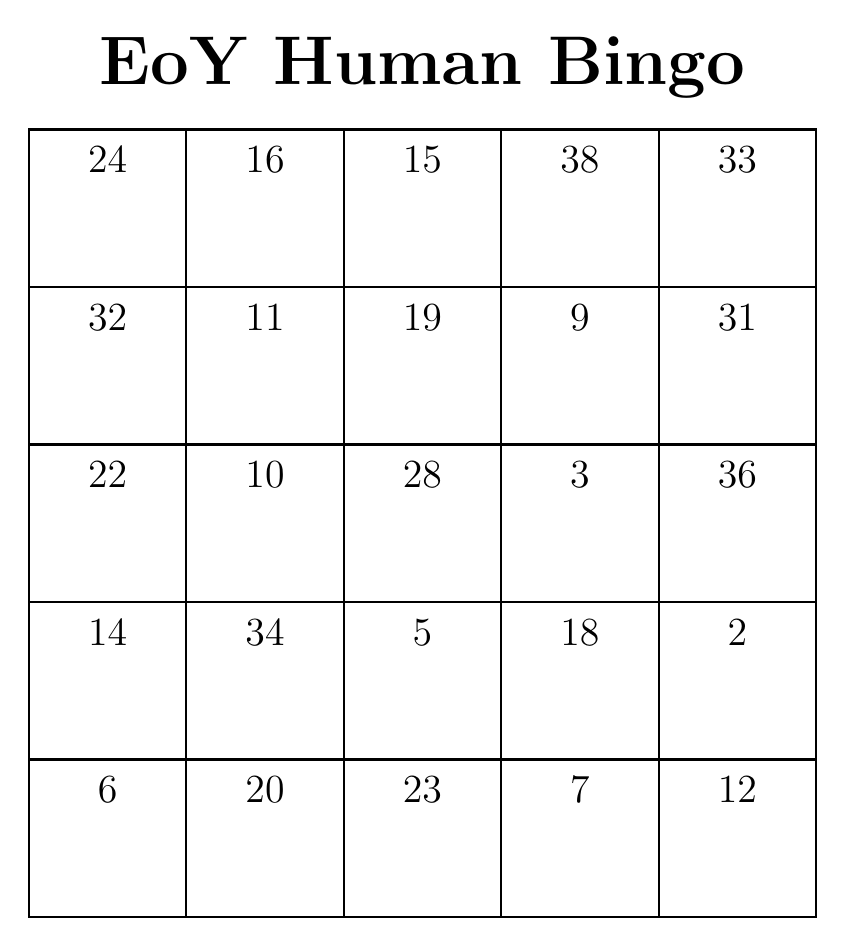
\begin{tikzpicture}
% Set the grid dimensions
\def\cellsize{2cm} % Each cell will be 2x2 cm

% Draw the grid and insert the numbers
\draw[thick] (0, 0) rectangle +(2, 2);
\node[anchor=north, font=\Large, align=center] at (1.0, 1.9) {24};
\draw[thick] (2, 0) rectangle +(2, 2);
\node[anchor=north, font=\Large, align=center] at (3.0, 1.9) {16};
\draw[thick] (4, 0) rectangle +(2, 2);
\node[anchor=north, font=\Large, align=center] at (5.0, 1.9) {15};
\draw[thick] (6, 0) rectangle +(2, 2);
\node[anchor=north, font=\Large, align=center] at (7.0, 1.9) {38};
\draw[thick] (8, 0) rectangle +(2, 2);
\node[anchor=north, font=\Large, align=center] at (9.0, 1.9) {33};
\draw[thick] (0, -2) rectangle +(2, 2);
\node[anchor=north, font=\Large, align=center] at (1.0, -0.1) {32};
\draw[thick] (2, -2) rectangle +(2, 2);
\node[anchor=north, font=\Large, align=center] at (3.0, -0.1) {11};
\draw[thick] (4, -2) rectangle +(2, 2);
\node[anchor=north, font=\Large, align=center] at (5.0, -0.1) {19};
\draw[thick] (6, -2) rectangle +(2, 2);
\node[anchor=north, font=\Large, align=center] at (7.0, -0.1) {9};
\draw[thick] (8, -2) rectangle +(2, 2);
\node[anchor=north, font=\Large, align=center] at (9.0, -0.1) {31};
\draw[thick] (0, -4) rectangle +(2, 2);
\node[anchor=north, font=\Large, align=center] at (1.0, -2.1) {22};
\draw[thick] (2, -4) rectangle +(2, 2);
\node[anchor=north, font=\Large, align=center] at (3.0, -2.1) {10};
\draw[thick] (4, -4) rectangle +(2, 2);
\node[anchor=north, font=\Large, align=center] at (5.0, -2.1) {28};
\draw[thick] (6, -4) rectangle +(2, 2);
\node[anchor=north, font=\Large, align=center] at (7.0, -2.1) {3};
\draw[thick] (8, -4) rectangle +(2, 2);
\node[anchor=north, font=\Large, align=center] at (9.0, -2.1) {36};
\draw[thick] (0, -6) rectangle +(2, 2);
\node[anchor=north, font=\Large, align=center] at (1.0, -4.1) {14};
\draw[thick] (2, -6) rectangle +(2, 2);
\node[anchor=north, font=\Large, align=center] at (3.0, -4.1) {34};
\draw[thick] (4, -6) rectangle +(2, 2);
\node[anchor=north, font=\Large, align=center] at (5.0, -4.1) {5};
\draw[thick] (6, -6) rectangle +(2, 2);
\node[anchor=north, font=\Large, align=center] at (7.0, -4.1) {18};
\draw[thick] (8, -6) rectangle +(2, 2);
\node[anchor=north, font=\Large, align=center] at (9.0, -4.1) {2};
\draw[thick] (0, -8) rectangle +(2, 2);
\node[anchor=north, font=\Large, align=center] at (1.0, -6.1) {6};
\draw[thick] (2, -8) rectangle +(2, 2);
\node[anchor=north, font=\Large, align=center] at (3.0, -6.1) {20};
\draw[thick] (4, -8) rectangle +(2, 2);
\node[anchor=north, font=\Large, align=center] at (5.0, -6.1) {23};
\draw[thick] (6, -8) rectangle +(2, 2);
\node[anchor=north, font=\Large, align=center] at (7.0, -6.1) {7};
\draw[thick] (8, -8) rectangle +(2, 2);
\node[anchor=north, font=\Large, align=center] at (9.0, -6.1) {12};
\node[anchor=north, font = \Huge] at (5.0, 3.3){\textbf{EoY Human Bingo}};
\end{tikzpicture}
\end{center}
\newpage\begin{center}
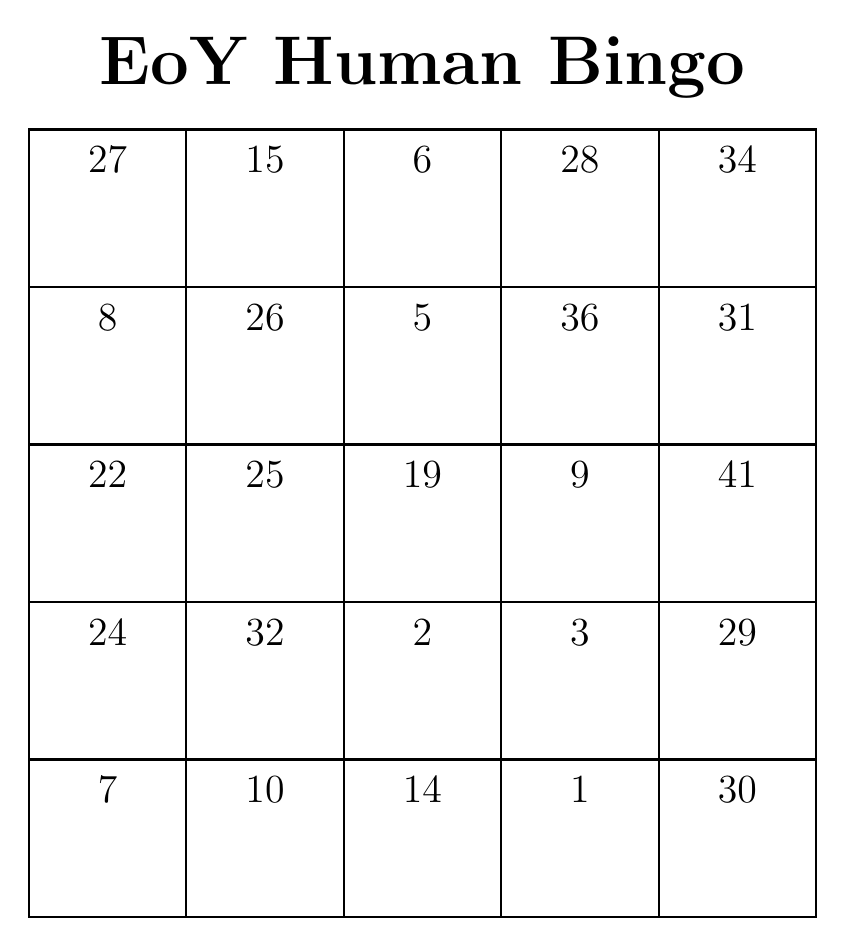
\begin{tikzpicture}
% Set the grid dimensions
\def\cellsize{2cm} % Each cell will be 2x2 cm

% Draw the grid and insert the numbers
\draw[thick] (0, 0) rectangle +(2, 2);
\node[anchor=north, font=\Large, align=center] at (1.0, 1.9) {27};
\draw[thick] (2, 0) rectangle +(2, 2);
\node[anchor=north, font=\Large, align=center] at (3.0, 1.9) {15};
\draw[thick] (4, 0) rectangle +(2, 2);
\node[anchor=north, font=\Large, align=center] at (5.0, 1.9) {6};
\draw[thick] (6, 0) rectangle +(2, 2);
\node[anchor=north, font=\Large, align=center] at (7.0, 1.9) {28};
\draw[thick] (8, 0) rectangle +(2, 2);
\node[anchor=north, font=\Large, align=center] at (9.0, 1.9) {34};
\draw[thick] (0, -2) rectangle +(2, 2);
\node[anchor=north, font=\Large, align=center] at (1.0, -0.1) {8};
\draw[thick] (2, -2) rectangle +(2, 2);
\node[anchor=north, font=\Large, align=center] at (3.0, -0.1) {26};
\draw[thick] (4, -2) rectangle +(2, 2);
\node[anchor=north, font=\Large, align=center] at (5.0, -0.1) {5};
\draw[thick] (6, -2) rectangle +(2, 2);
\node[anchor=north, font=\Large, align=center] at (7.0, -0.1) {36};
\draw[thick] (8, -2) rectangle +(2, 2);
\node[anchor=north, font=\Large, align=center] at (9.0, -0.1) {31};
\draw[thick] (0, -4) rectangle +(2, 2);
\node[anchor=north, font=\Large, align=center] at (1.0, -2.1) {22};
\draw[thick] (2, -4) rectangle +(2, 2);
\node[anchor=north, font=\Large, align=center] at (3.0, -2.1) {25};
\draw[thick] (4, -4) rectangle +(2, 2);
\node[anchor=north, font=\Large, align=center] at (5.0, -2.1) {19};
\draw[thick] (6, -4) rectangle +(2, 2);
\node[anchor=north, font=\Large, align=center] at (7.0, -2.1) {9};
\draw[thick] (8, -4) rectangle +(2, 2);
\node[anchor=north, font=\Large, align=center] at (9.0, -2.1) {41};
\draw[thick] (0, -6) rectangle +(2, 2);
\node[anchor=north, font=\Large, align=center] at (1.0, -4.1) {24};
\draw[thick] (2, -6) rectangle +(2, 2);
\node[anchor=north, font=\Large, align=center] at (3.0, -4.1) {32};
\draw[thick] (4, -6) rectangle +(2, 2);
\node[anchor=north, font=\Large, align=center] at (5.0, -4.1) {2};
\draw[thick] (6, -6) rectangle +(2, 2);
\node[anchor=north, font=\Large, align=center] at (7.0, -4.1) {3};
\draw[thick] (8, -6) rectangle +(2, 2);
\node[anchor=north, font=\Large, align=center] at (9.0, -4.1) {29};
\draw[thick] (0, -8) rectangle +(2, 2);
\node[anchor=north, font=\Large, align=center] at (1.0, -6.1) {7};
\draw[thick] (2, -8) rectangle +(2, 2);
\node[anchor=north, font=\Large, align=center] at (3.0, -6.1) {10};
\draw[thick] (4, -8) rectangle +(2, 2);
\node[anchor=north, font=\Large, align=center] at (5.0, -6.1) {14};
\draw[thick] (6, -8) rectangle +(2, 2);
\node[anchor=north, font=\Large, align=center] at (7.0, -6.1) {1};
\draw[thick] (8, -8) rectangle +(2, 2);
\node[anchor=north, font=\Large, align=center] at (9.0, -6.1) {30};
\node[anchor=north, font = \Huge] at (5.0, 3.3){\textbf{EoY Human Bingo}};
\end{tikzpicture}
\end{center}
\newpage\begin{center}
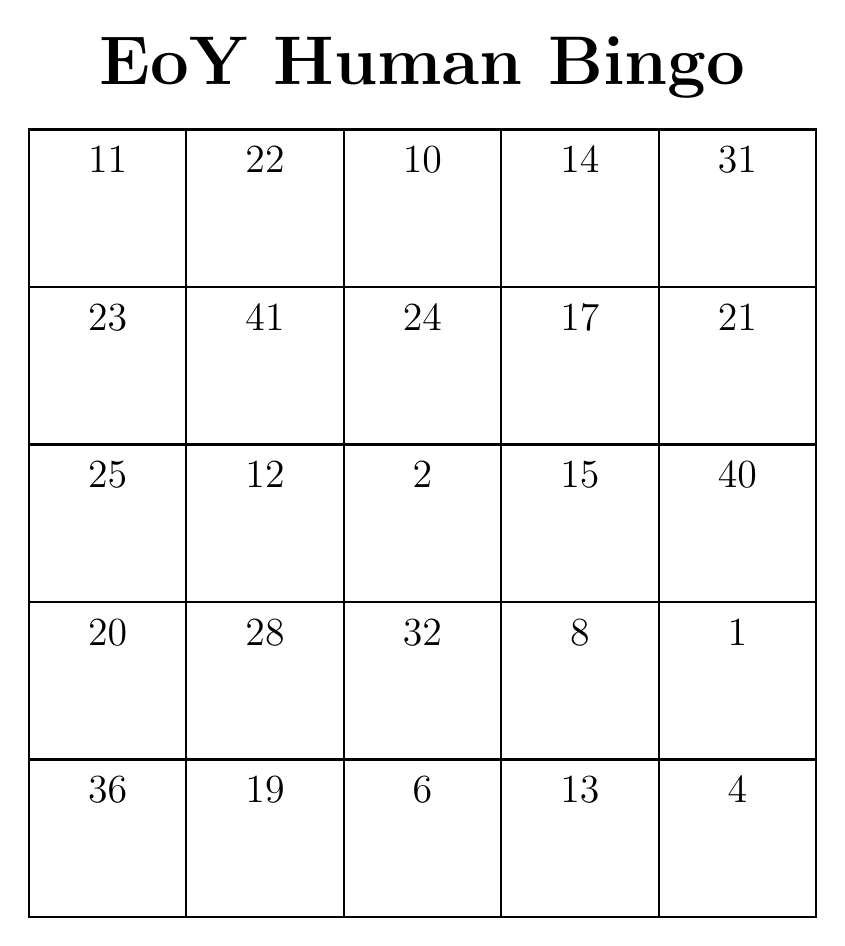
\begin{tikzpicture}
% Set the grid dimensions
\def\cellsize{2cm} % Each cell will be 2x2 cm

% Draw the grid and insert the numbers
\draw[thick] (0, 0) rectangle +(2, 2);
\node[anchor=north, font=\Large, align=center] at (1.0, 1.9) {11};
\draw[thick] (2, 0) rectangle +(2, 2);
\node[anchor=north, font=\Large, align=center] at (3.0, 1.9) {22};
\draw[thick] (4, 0) rectangle +(2, 2);
\node[anchor=north, font=\Large, align=center] at (5.0, 1.9) {10};
\draw[thick] (6, 0) rectangle +(2, 2);
\node[anchor=north, font=\Large, align=center] at (7.0, 1.9) {14};
\draw[thick] (8, 0) rectangle +(2, 2);
\node[anchor=north, font=\Large, align=center] at (9.0, 1.9) {31};
\draw[thick] (0, -2) rectangle +(2, 2);
\node[anchor=north, font=\Large, align=center] at (1.0, -0.1) {23};
\draw[thick] (2, -2) rectangle +(2, 2);
\node[anchor=north, font=\Large, align=center] at (3.0, -0.1) {41};
\draw[thick] (4, -2) rectangle +(2, 2);
\node[anchor=north, font=\Large, align=center] at (5.0, -0.1) {24};
\draw[thick] (6, -2) rectangle +(2, 2);
\node[anchor=north, font=\Large, align=center] at (7.0, -0.1) {17};
\draw[thick] (8, -2) rectangle +(2, 2);
\node[anchor=north, font=\Large, align=center] at (9.0, -0.1) {21};
\draw[thick] (0, -4) rectangle +(2, 2);
\node[anchor=north, font=\Large, align=center] at (1.0, -2.1) {25};
\draw[thick] (2, -4) rectangle +(2, 2);
\node[anchor=north, font=\Large, align=center] at (3.0, -2.1) {12};
\draw[thick] (4, -4) rectangle +(2, 2);
\node[anchor=north, font=\Large, align=center] at (5.0, -2.1) {2};
\draw[thick] (6, -4) rectangle +(2, 2);
\node[anchor=north, font=\Large, align=center] at (7.0, -2.1) {15};
\draw[thick] (8, -4) rectangle +(2, 2);
\node[anchor=north, font=\Large, align=center] at (9.0, -2.1) {40};
\draw[thick] (0, -6) rectangle +(2, 2);
\node[anchor=north, font=\Large, align=center] at (1.0, -4.1) {20};
\draw[thick] (2, -6) rectangle +(2, 2);
\node[anchor=north, font=\Large, align=center] at (3.0, -4.1) {28};
\draw[thick] (4, -6) rectangle +(2, 2);
\node[anchor=north, font=\Large, align=center] at (5.0, -4.1) {32};
\draw[thick] (6, -6) rectangle +(2, 2);
\node[anchor=north, font=\Large, align=center] at (7.0, -4.1) {8};
\draw[thick] (8, -6) rectangle +(2, 2);
\node[anchor=north, font=\Large, align=center] at (9.0, -4.1) {1};
\draw[thick] (0, -8) rectangle +(2, 2);
\node[anchor=north, font=\Large, align=center] at (1.0, -6.1) {36};
\draw[thick] (2, -8) rectangle +(2, 2);
\node[anchor=north, font=\Large, align=center] at (3.0, -6.1) {19};
\draw[thick] (4, -8) rectangle +(2, 2);
\node[anchor=north, font=\Large, align=center] at (5.0, -6.1) {6};
\draw[thick] (6, -8) rectangle +(2, 2);
\node[anchor=north, font=\Large, align=center] at (7.0, -6.1) {13};
\draw[thick] (8, -8) rectangle +(2, 2);
\node[anchor=north, font=\Large, align=center] at (9.0, -6.1) {4};
\node[anchor=north, font = \Huge] at (5.0, 3.3){\textbf{EoY Human Bingo}};
\end{tikzpicture}
\end{center}
\newpage\begin{center}
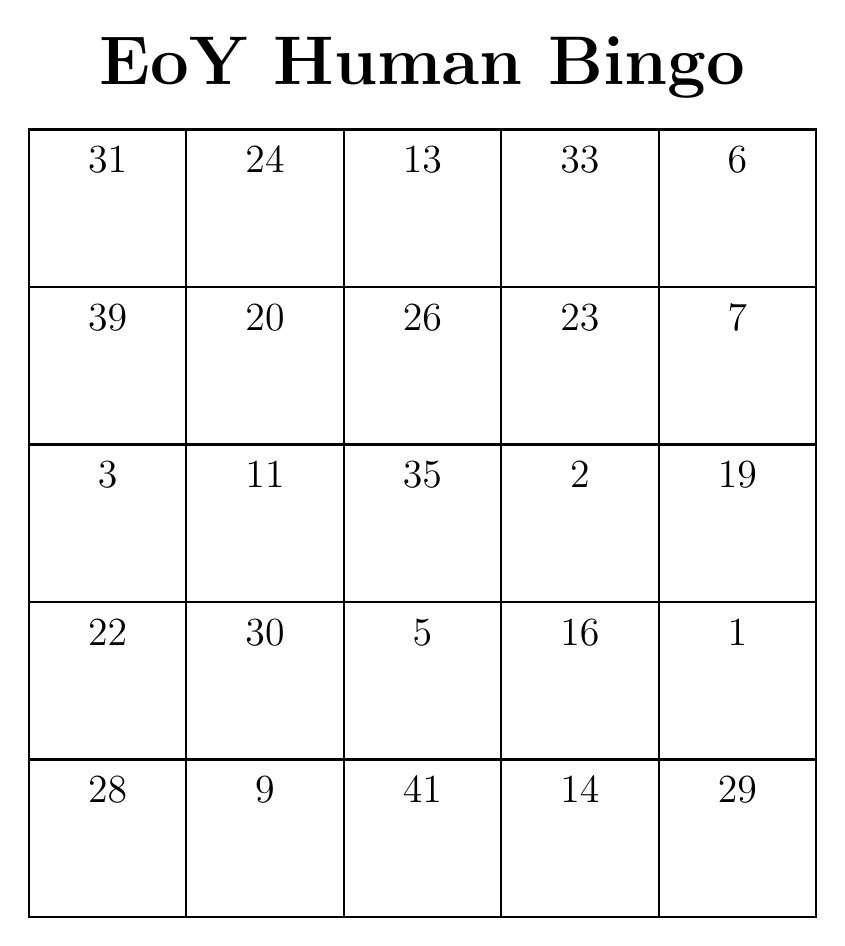
\begin{tikzpicture}
% Set the grid dimensions
\def\cellsize{2cm} % Each cell will be 2x2 cm

% Draw the grid and insert the numbers
\draw[thick] (0, 0) rectangle +(2, 2);
\node[anchor=north, font=\Large, align=center] at (1.0, 1.9) {31};
\draw[thick] (2, 0) rectangle +(2, 2);
\node[anchor=north, font=\Large, align=center] at (3.0, 1.9) {24};
\draw[thick] (4, 0) rectangle +(2, 2);
\node[anchor=north, font=\Large, align=center] at (5.0, 1.9) {13};
\draw[thick] (6, 0) rectangle +(2, 2);
\node[anchor=north, font=\Large, align=center] at (7.0, 1.9) {33};
\draw[thick] (8, 0) rectangle +(2, 2);
\node[anchor=north, font=\Large, align=center] at (9.0, 1.9) {6};
\draw[thick] (0, -2) rectangle +(2, 2);
\node[anchor=north, font=\Large, align=center] at (1.0, -0.1) {39};
\draw[thick] (2, -2) rectangle +(2, 2);
\node[anchor=north, font=\Large, align=center] at (3.0, -0.1) {20};
\draw[thick] (4, -2) rectangle +(2, 2);
\node[anchor=north, font=\Large, align=center] at (5.0, -0.1) {26};
\draw[thick] (6, -2) rectangle +(2, 2);
\node[anchor=north, font=\Large, align=center] at (7.0, -0.1) {23};
\draw[thick] (8, -2) rectangle +(2, 2);
\node[anchor=north, font=\Large, align=center] at (9.0, -0.1) {7};
\draw[thick] (0, -4) rectangle +(2, 2);
\node[anchor=north, font=\Large, align=center] at (1.0, -2.1) {3};
\draw[thick] (2, -4) rectangle +(2, 2);
\node[anchor=north, font=\Large, align=center] at (3.0, -2.1) {11};
\draw[thick] (4, -4) rectangle +(2, 2);
\node[anchor=north, font=\Large, align=center] at (5.0, -2.1) {35};
\draw[thick] (6, -4) rectangle +(2, 2);
\node[anchor=north, font=\Large, align=center] at (7.0, -2.1) {2};
\draw[thick] (8, -4) rectangle +(2, 2);
\node[anchor=north, font=\Large, align=center] at (9.0, -2.1) {19};
\draw[thick] (0, -6) rectangle +(2, 2);
\node[anchor=north, font=\Large, align=center] at (1.0, -4.1) {22};
\draw[thick] (2, -6) rectangle +(2, 2);
\node[anchor=north, font=\Large, align=center] at (3.0, -4.1) {30};
\draw[thick] (4, -6) rectangle +(2, 2);
\node[anchor=north, font=\Large, align=center] at (5.0, -4.1) {5};
\draw[thick] (6, -6) rectangle +(2, 2);
\node[anchor=north, font=\Large, align=center] at (7.0, -4.1) {16};
\draw[thick] (8, -6) rectangle +(2, 2);
\node[anchor=north, font=\Large, align=center] at (9.0, -4.1) {1};
\draw[thick] (0, -8) rectangle +(2, 2);
\node[anchor=north, font=\Large, align=center] at (1.0, -6.1) {28};
\draw[thick] (2, -8) rectangle +(2, 2);
\node[anchor=north, font=\Large, align=center] at (3.0, -6.1) {9};
\draw[thick] (4, -8) rectangle +(2, 2);
\node[anchor=north, font=\Large, align=center] at (5.0, -6.1) {41};
\draw[thick] (6, -8) rectangle +(2, 2);
\node[anchor=north, font=\Large, align=center] at (7.0, -6.1) {14};
\draw[thick] (8, -8) rectangle +(2, 2);
\node[anchor=north, font=\Large, align=center] at (9.0, -6.1) {29};
\node[anchor=north, font = \Huge] at (5.0, 3.3){\textbf{EoY Human Bingo}};
\end{tikzpicture}
\end{center}
\newpage\begin{center}
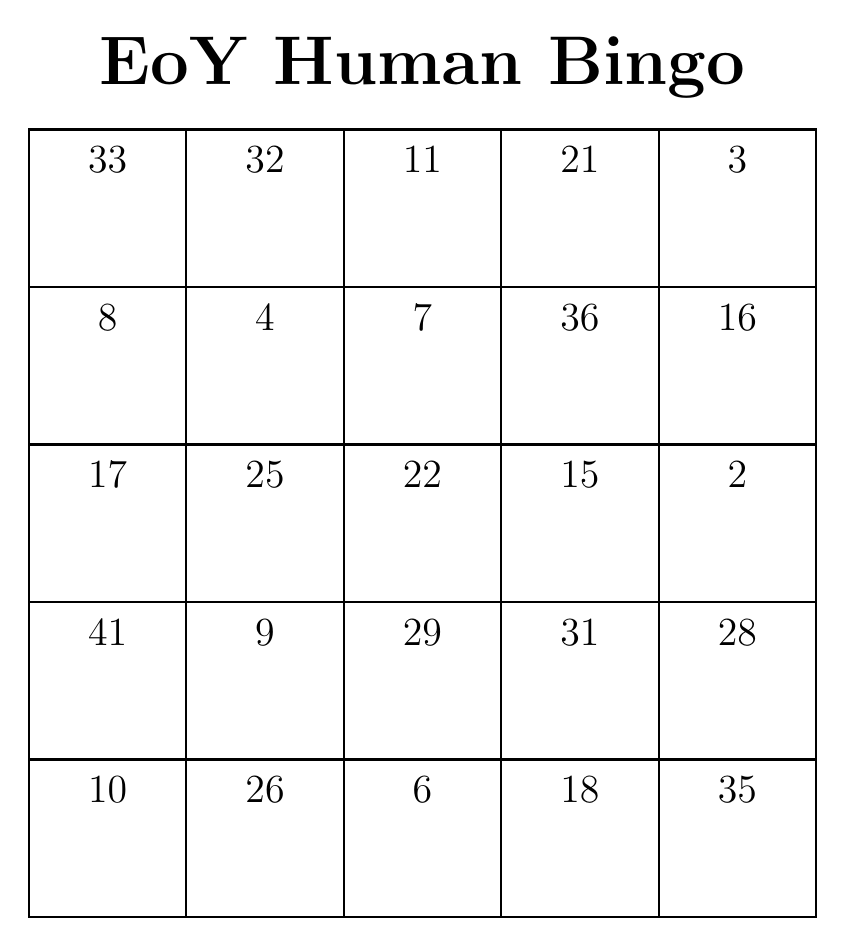
\begin{tikzpicture}
% Set the grid dimensions
\def\cellsize{2cm} % Each cell will be 2x2 cm

% Draw the grid and insert the numbers
\draw[thick] (0, 0) rectangle +(2, 2);
\node[anchor=north, font=\Large, align=center] at (1.0, 1.9) {33};
\draw[thick] (2, 0) rectangle +(2, 2);
\node[anchor=north, font=\Large, align=center] at (3.0, 1.9) {32};
\draw[thick] (4, 0) rectangle +(2, 2);
\node[anchor=north, font=\Large, align=center] at (5.0, 1.9) {11};
\draw[thick] (6, 0) rectangle +(2, 2);
\node[anchor=north, font=\Large, align=center] at (7.0, 1.9) {21};
\draw[thick] (8, 0) rectangle +(2, 2);
\node[anchor=north, font=\Large, align=center] at (9.0, 1.9) {3};
\draw[thick] (0, -2) rectangle +(2, 2);
\node[anchor=north, font=\Large, align=center] at (1.0, -0.1) {8};
\draw[thick] (2, -2) rectangle +(2, 2);
\node[anchor=north, font=\Large, align=center] at (3.0, -0.1) {4};
\draw[thick] (4, -2) rectangle +(2, 2);
\node[anchor=north, font=\Large, align=center] at (5.0, -0.1) {7};
\draw[thick] (6, -2) rectangle +(2, 2);
\node[anchor=north, font=\Large, align=center] at (7.0, -0.1) {36};
\draw[thick] (8, -2) rectangle +(2, 2);
\node[anchor=north, font=\Large, align=center] at (9.0, -0.1) {16};
\draw[thick] (0, -4) rectangle +(2, 2);
\node[anchor=north, font=\Large, align=center] at (1.0, -2.1) {17};
\draw[thick] (2, -4) rectangle +(2, 2);
\node[anchor=north, font=\Large, align=center] at (3.0, -2.1) {25};
\draw[thick] (4, -4) rectangle +(2, 2);
\node[anchor=north, font=\Large, align=center] at (5.0, -2.1) {22};
\draw[thick] (6, -4) rectangle +(2, 2);
\node[anchor=north, font=\Large, align=center] at (7.0, -2.1) {15};
\draw[thick] (8, -4) rectangle +(2, 2);
\node[anchor=north, font=\Large, align=center] at (9.0, -2.1) {2};
\draw[thick] (0, -6) rectangle +(2, 2);
\node[anchor=north, font=\Large, align=center] at (1.0, -4.1) {41};
\draw[thick] (2, -6) rectangle +(2, 2);
\node[anchor=north, font=\Large, align=center] at (3.0, -4.1) {9};
\draw[thick] (4, -6) rectangle +(2, 2);
\node[anchor=north, font=\Large, align=center] at (5.0, -4.1) {29};
\draw[thick] (6, -6) rectangle +(2, 2);
\node[anchor=north, font=\Large, align=center] at (7.0, -4.1) {31};
\draw[thick] (8, -6) rectangle +(2, 2);
\node[anchor=north, font=\Large, align=center] at (9.0, -4.1) {28};
\draw[thick] (0, -8) rectangle +(2, 2);
\node[anchor=north, font=\Large, align=center] at (1.0, -6.1) {10};
\draw[thick] (2, -8) rectangle +(2, 2);
\node[anchor=north, font=\Large, align=center] at (3.0, -6.1) {26};
\draw[thick] (4, -8) rectangle +(2, 2);
\node[anchor=north, font=\Large, align=center] at (5.0, -6.1) {6};
\draw[thick] (6, -8) rectangle +(2, 2);
\node[anchor=north, font=\Large, align=center] at (7.0, -6.1) {18};
\draw[thick] (8, -8) rectangle +(2, 2);
\node[anchor=north, font=\Large, align=center] at (9.0, -6.1) {35};
\node[anchor=north, font = \Huge] at (5.0, 3.3){\textbf{EoY Human Bingo}};
\end{tikzpicture}
\end{center}
\newpage\begin{center}
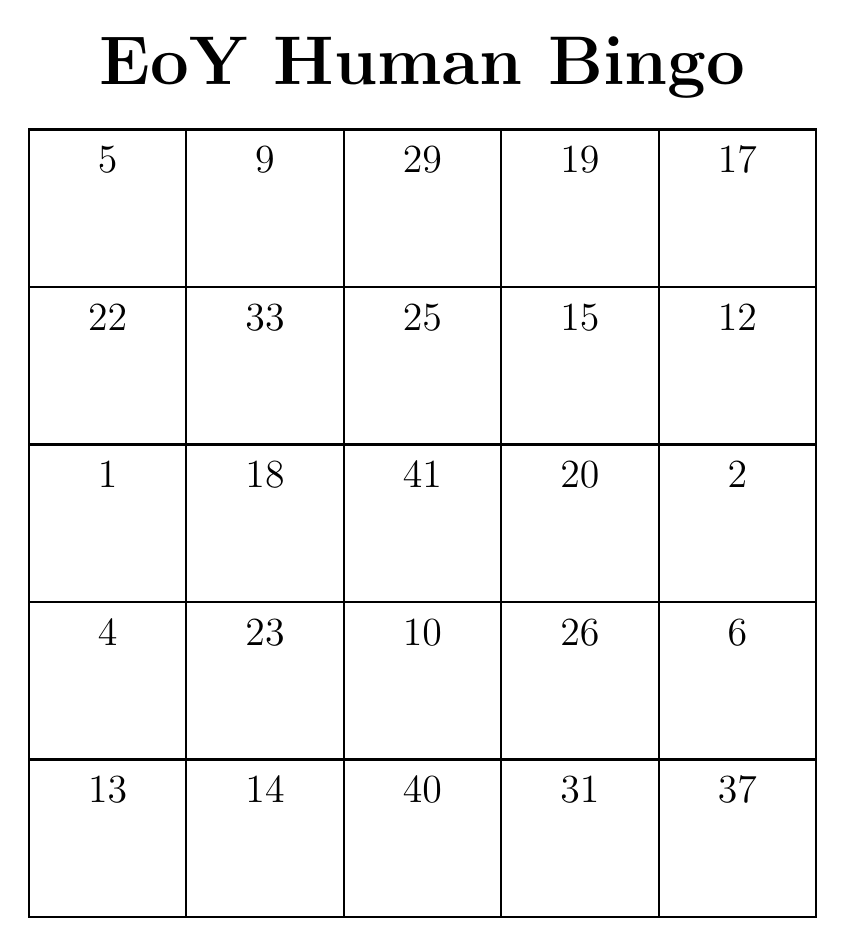
\begin{tikzpicture}
% Set the grid dimensions
\def\cellsize{2cm} % Each cell will be 2x2 cm

% Draw the grid and insert the numbers
\draw[thick] (0, 0) rectangle +(2, 2);
\node[anchor=north, font=\Large, align=center] at (1.0, 1.9) {5};
\draw[thick] (2, 0) rectangle +(2, 2);
\node[anchor=north, font=\Large, align=center] at (3.0, 1.9) {9};
\draw[thick] (4, 0) rectangle +(2, 2);
\node[anchor=north, font=\Large, align=center] at (5.0, 1.9) {29};
\draw[thick] (6, 0) rectangle +(2, 2);
\node[anchor=north, font=\Large, align=center] at (7.0, 1.9) {19};
\draw[thick] (8, 0) rectangle +(2, 2);
\node[anchor=north, font=\Large, align=center] at (9.0, 1.9) {17};
\draw[thick] (0, -2) rectangle +(2, 2);
\node[anchor=north, font=\Large, align=center] at (1.0, -0.1) {22};
\draw[thick] (2, -2) rectangle +(2, 2);
\node[anchor=north, font=\Large, align=center] at (3.0, -0.1) {33};
\draw[thick] (4, -2) rectangle +(2, 2);
\node[anchor=north, font=\Large, align=center] at (5.0, -0.1) {25};
\draw[thick] (6, -2) rectangle +(2, 2);
\node[anchor=north, font=\Large, align=center] at (7.0, -0.1) {15};
\draw[thick] (8, -2) rectangle +(2, 2);
\node[anchor=north, font=\Large, align=center] at (9.0, -0.1) {12};
\draw[thick] (0, -4) rectangle +(2, 2);
\node[anchor=north, font=\Large, align=center] at (1.0, -2.1) {1};
\draw[thick] (2, -4) rectangle +(2, 2);
\node[anchor=north, font=\Large, align=center] at (3.0, -2.1) {18};
\draw[thick] (4, -4) rectangle +(2, 2);
\node[anchor=north, font=\Large, align=center] at (5.0, -2.1) {41};
\draw[thick] (6, -4) rectangle +(2, 2);
\node[anchor=north, font=\Large, align=center] at (7.0, -2.1) {20};
\draw[thick] (8, -4) rectangle +(2, 2);
\node[anchor=north, font=\Large, align=center] at (9.0, -2.1) {2};
\draw[thick] (0, -6) rectangle +(2, 2);
\node[anchor=north, font=\Large, align=center] at (1.0, -4.1) {4};
\draw[thick] (2, -6) rectangle +(2, 2);
\node[anchor=north, font=\Large, align=center] at (3.0, -4.1) {23};
\draw[thick] (4, -6) rectangle +(2, 2);
\node[anchor=north, font=\Large, align=center] at (5.0, -4.1) {10};
\draw[thick] (6, -6) rectangle +(2, 2);
\node[anchor=north, font=\Large, align=center] at (7.0, -4.1) {26};
\draw[thick] (8, -6) rectangle +(2, 2);
\node[anchor=north, font=\Large, align=center] at (9.0, -4.1) {6};
\draw[thick] (0, -8) rectangle +(2, 2);
\node[anchor=north, font=\Large, align=center] at (1.0, -6.1) {13};
\draw[thick] (2, -8) rectangle +(2, 2);
\node[anchor=north, font=\Large, align=center] at (3.0, -6.1) {14};
\draw[thick] (4, -8) rectangle +(2, 2);
\node[anchor=north, font=\Large, align=center] at (5.0, -6.1) {40};
\draw[thick] (6, -8) rectangle +(2, 2);
\node[anchor=north, font=\Large, align=center] at (7.0, -6.1) {31};
\draw[thick] (8, -8) rectangle +(2, 2);
\node[anchor=north, font=\Large, align=center] at (9.0, -6.1) {37};
\node[anchor=north, font = \Huge] at (5.0, 3.3){\textbf{EoY Human Bingo}};
\end{tikzpicture}
\end{center}
\newpage\begin{center}
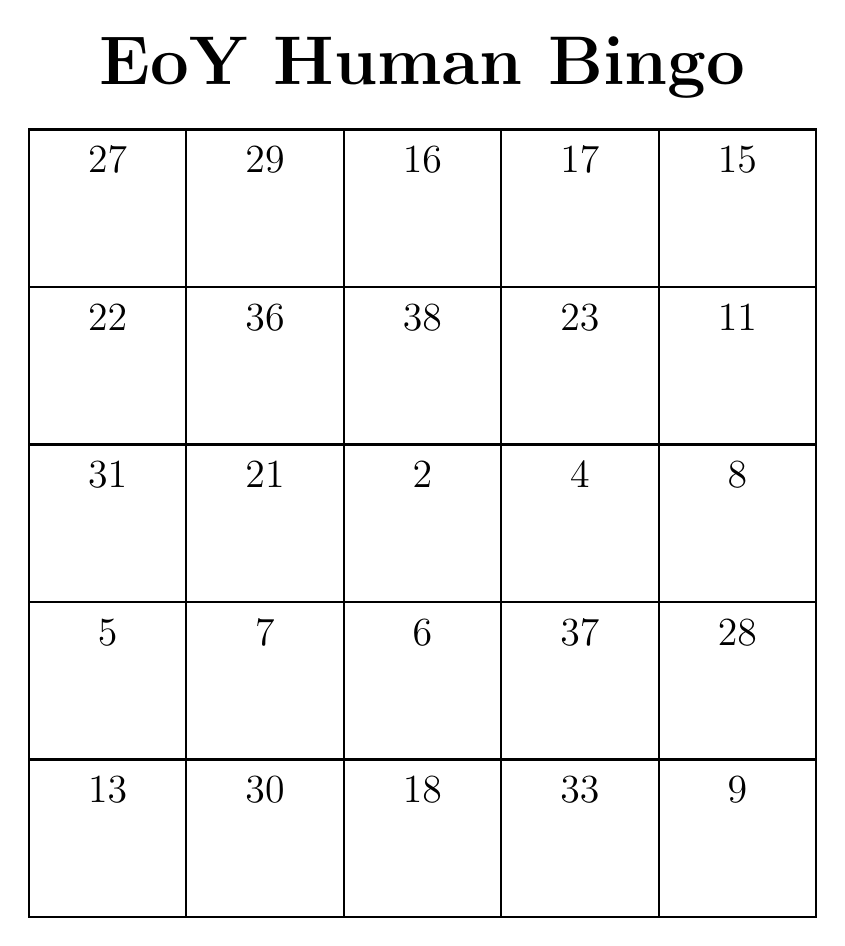
\begin{tikzpicture}
% Set the grid dimensions
\def\cellsize{2cm} % Each cell will be 2x2 cm

% Draw the grid and insert the numbers
\draw[thick] (0, 0) rectangle +(2, 2);
\node[anchor=north, font=\Large, align=center] at (1.0, 1.9) {27};
\draw[thick] (2, 0) rectangle +(2, 2);
\node[anchor=north, font=\Large, align=center] at (3.0, 1.9) {29};
\draw[thick] (4, 0) rectangle +(2, 2);
\node[anchor=north, font=\Large, align=center] at (5.0, 1.9) {16};
\draw[thick] (6, 0) rectangle +(2, 2);
\node[anchor=north, font=\Large, align=center] at (7.0, 1.9) {17};
\draw[thick] (8, 0) rectangle +(2, 2);
\node[anchor=north, font=\Large, align=center] at (9.0, 1.9) {15};
\draw[thick] (0, -2) rectangle +(2, 2);
\node[anchor=north, font=\Large, align=center] at (1.0, -0.1) {22};
\draw[thick] (2, -2) rectangle +(2, 2);
\node[anchor=north, font=\Large, align=center] at (3.0, -0.1) {36};
\draw[thick] (4, -2) rectangle +(2, 2);
\node[anchor=north, font=\Large, align=center] at (5.0, -0.1) {38};
\draw[thick] (6, -2) rectangle +(2, 2);
\node[anchor=north, font=\Large, align=center] at (7.0, -0.1) {23};
\draw[thick] (8, -2) rectangle +(2, 2);
\node[anchor=north, font=\Large, align=center] at (9.0, -0.1) {11};
\draw[thick] (0, -4) rectangle +(2, 2);
\node[anchor=north, font=\Large, align=center] at (1.0, -2.1) {31};
\draw[thick] (2, -4) rectangle +(2, 2);
\node[anchor=north, font=\Large, align=center] at (3.0, -2.1) {21};
\draw[thick] (4, -4) rectangle +(2, 2);
\node[anchor=north, font=\Large, align=center] at (5.0, -2.1) {2};
\draw[thick] (6, -4) rectangle +(2, 2);
\node[anchor=north, font=\Large, align=center] at (7.0, -2.1) {4};
\draw[thick] (8, -4) rectangle +(2, 2);
\node[anchor=north, font=\Large, align=center] at (9.0, -2.1) {8};
\draw[thick] (0, -6) rectangle +(2, 2);
\node[anchor=north, font=\Large, align=center] at (1.0, -4.1) {5};
\draw[thick] (2, -6) rectangle +(2, 2);
\node[anchor=north, font=\Large, align=center] at (3.0, -4.1) {7};
\draw[thick] (4, -6) rectangle +(2, 2);
\node[anchor=north, font=\Large, align=center] at (5.0, -4.1) {6};
\draw[thick] (6, -6) rectangle +(2, 2);
\node[anchor=north, font=\Large, align=center] at (7.0, -4.1) {37};
\draw[thick] (8, -6) rectangle +(2, 2);
\node[anchor=north, font=\Large, align=center] at (9.0, -4.1) {28};
\draw[thick] (0, -8) rectangle +(2, 2);
\node[anchor=north, font=\Large, align=center] at (1.0, -6.1) {13};
\draw[thick] (2, -8) rectangle +(2, 2);
\node[anchor=north, font=\Large, align=center] at (3.0, -6.1) {30};
\draw[thick] (4, -8) rectangle +(2, 2);
\node[anchor=north, font=\Large, align=center] at (5.0, -6.1) {18};
\draw[thick] (6, -8) rectangle +(2, 2);
\node[anchor=north, font=\Large, align=center] at (7.0, -6.1) {33};
\draw[thick] (8, -8) rectangle +(2, 2);
\node[anchor=north, font=\Large, align=center] at (9.0, -6.1) {9};
\node[anchor=north, font = \Huge] at (5.0, 3.3){\textbf{EoY Human Bingo}};
\end{tikzpicture}
\end{center}
\newpage\begin{center}
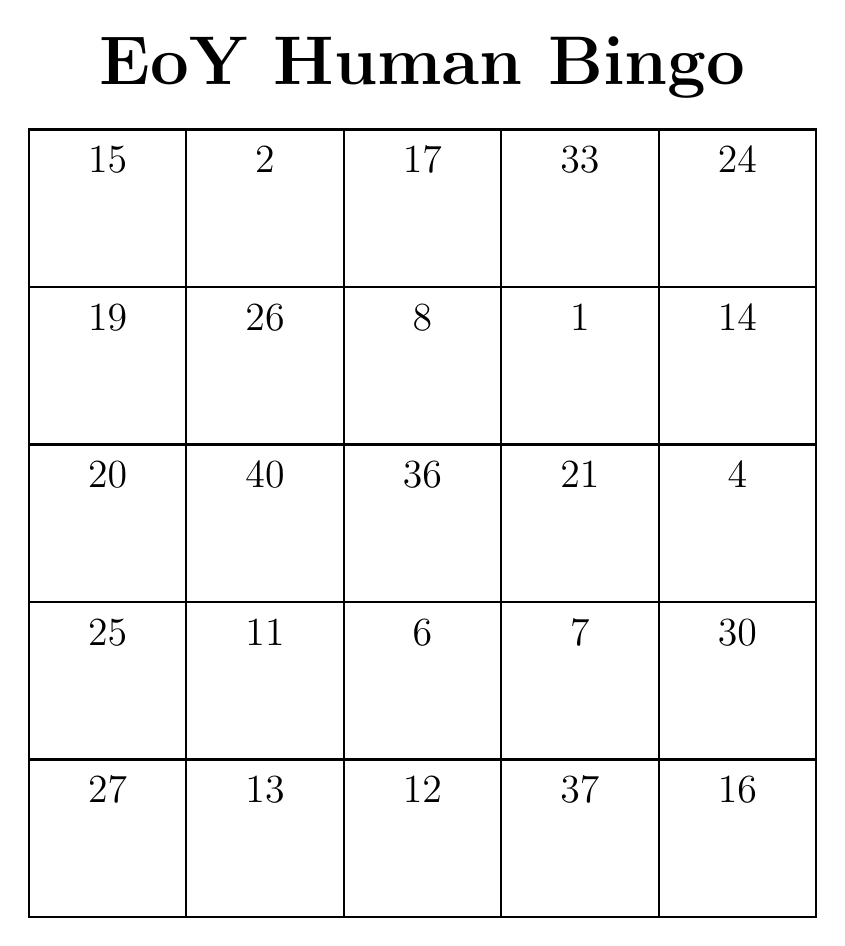
\begin{tikzpicture}
% Set the grid dimensions
\def\cellsize{2cm} % Each cell will be 2x2 cm

% Draw the grid and insert the numbers
\draw[thick] (0, 0) rectangle +(2, 2);
\node[anchor=north, font=\Large, align=center] at (1.0, 1.9) {15};
\draw[thick] (2, 0) rectangle +(2, 2);
\node[anchor=north, font=\Large, align=center] at (3.0, 1.9) {2};
\draw[thick] (4, 0) rectangle +(2, 2);
\node[anchor=north, font=\Large, align=center] at (5.0, 1.9) {17};
\draw[thick] (6, 0) rectangle +(2, 2);
\node[anchor=north, font=\Large, align=center] at (7.0, 1.9) {33};
\draw[thick] (8, 0) rectangle +(2, 2);
\node[anchor=north, font=\Large, align=center] at (9.0, 1.9) {24};
\draw[thick] (0, -2) rectangle +(2, 2);
\node[anchor=north, font=\Large, align=center] at (1.0, -0.1) {19};
\draw[thick] (2, -2) rectangle +(2, 2);
\node[anchor=north, font=\Large, align=center] at (3.0, -0.1) {26};
\draw[thick] (4, -2) rectangle +(2, 2);
\node[anchor=north, font=\Large, align=center] at (5.0, -0.1) {8};
\draw[thick] (6, -2) rectangle +(2, 2);
\node[anchor=north, font=\Large, align=center] at (7.0, -0.1) {1};
\draw[thick] (8, -2) rectangle +(2, 2);
\node[anchor=north, font=\Large, align=center] at (9.0, -0.1) {14};
\draw[thick] (0, -4) rectangle +(2, 2);
\node[anchor=north, font=\Large, align=center] at (1.0, -2.1) {20};
\draw[thick] (2, -4) rectangle +(2, 2);
\node[anchor=north, font=\Large, align=center] at (3.0, -2.1) {40};
\draw[thick] (4, -4) rectangle +(2, 2);
\node[anchor=north, font=\Large, align=center] at (5.0, -2.1) {36};
\draw[thick] (6, -4) rectangle +(2, 2);
\node[anchor=north, font=\Large, align=center] at (7.0, -2.1) {21};
\draw[thick] (8, -4) rectangle +(2, 2);
\node[anchor=north, font=\Large, align=center] at (9.0, -2.1) {4};
\draw[thick] (0, -6) rectangle +(2, 2);
\node[anchor=north, font=\Large, align=center] at (1.0, -4.1) {25};
\draw[thick] (2, -6) rectangle +(2, 2);
\node[anchor=north, font=\Large, align=center] at (3.0, -4.1) {11};
\draw[thick] (4, -6) rectangle +(2, 2);
\node[anchor=north, font=\Large, align=center] at (5.0, -4.1) {6};
\draw[thick] (6, -6) rectangle +(2, 2);
\node[anchor=north, font=\Large, align=center] at (7.0, -4.1) {7};
\draw[thick] (8, -6) rectangle +(2, 2);
\node[anchor=north, font=\Large, align=center] at (9.0, -4.1) {30};
\draw[thick] (0, -8) rectangle +(2, 2);
\node[anchor=north, font=\Large, align=center] at (1.0, -6.1) {27};
\draw[thick] (2, -8) rectangle +(2, 2);
\node[anchor=north, font=\Large, align=center] at (3.0, -6.1) {13};
\draw[thick] (4, -8) rectangle +(2, 2);
\node[anchor=north, font=\Large, align=center] at (5.0, -6.1) {12};
\draw[thick] (6, -8) rectangle +(2, 2);
\node[anchor=north, font=\Large, align=center] at (7.0, -6.1) {37};
\draw[thick] (8, -8) rectangle +(2, 2);
\node[anchor=north, font=\Large, align=center] at (9.0, -6.1) {16};
\node[anchor=north, font = \Huge] at (5.0, 3.3){\textbf{EoY Human Bingo}};
\end{tikzpicture}
\end{center}
\newpage\begin{center}
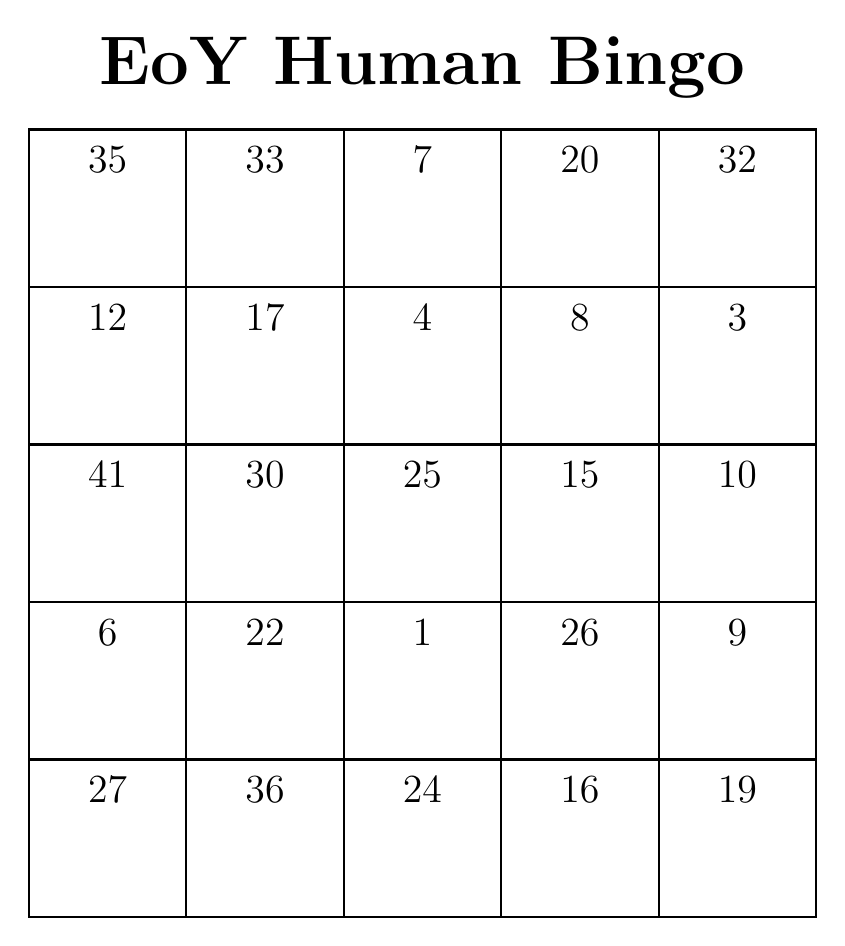
\begin{tikzpicture}
% Set the grid dimensions
\def\cellsize{2cm} % Each cell will be 2x2 cm

% Draw the grid and insert the numbers
\draw[thick] (0, 0) rectangle +(2, 2);
\node[anchor=north, font=\Large, align=center] at (1.0, 1.9) {35};
\draw[thick] (2, 0) rectangle +(2, 2);
\node[anchor=north, font=\Large, align=center] at (3.0, 1.9) {33};
\draw[thick] (4, 0) rectangle +(2, 2);
\node[anchor=north, font=\Large, align=center] at (5.0, 1.9) {7};
\draw[thick] (6, 0) rectangle +(2, 2);
\node[anchor=north, font=\Large, align=center] at (7.0, 1.9) {20};
\draw[thick] (8, 0) rectangle +(2, 2);
\node[anchor=north, font=\Large, align=center] at (9.0, 1.9) {32};
\draw[thick] (0, -2) rectangle +(2, 2);
\node[anchor=north, font=\Large, align=center] at (1.0, -0.1) {12};
\draw[thick] (2, -2) rectangle +(2, 2);
\node[anchor=north, font=\Large, align=center] at (3.0, -0.1) {17};
\draw[thick] (4, -2) rectangle +(2, 2);
\node[anchor=north, font=\Large, align=center] at (5.0, -0.1) {4};
\draw[thick] (6, -2) rectangle +(2, 2);
\node[anchor=north, font=\Large, align=center] at (7.0, -0.1) {8};
\draw[thick] (8, -2) rectangle +(2, 2);
\node[anchor=north, font=\Large, align=center] at (9.0, -0.1) {3};
\draw[thick] (0, -4) rectangle +(2, 2);
\node[anchor=north, font=\Large, align=center] at (1.0, -2.1) {41};
\draw[thick] (2, -4) rectangle +(2, 2);
\node[anchor=north, font=\Large, align=center] at (3.0, -2.1) {30};
\draw[thick] (4, -4) rectangle +(2, 2);
\node[anchor=north, font=\Large, align=center] at (5.0, -2.1) {25};
\draw[thick] (6, -4) rectangle +(2, 2);
\node[anchor=north, font=\Large, align=center] at (7.0, -2.1) {15};
\draw[thick] (8, -4) rectangle +(2, 2);
\node[anchor=north, font=\Large, align=center] at (9.0, -2.1) {10};
\draw[thick] (0, -6) rectangle +(2, 2);
\node[anchor=north, font=\Large, align=center] at (1.0, -4.1) {6};
\draw[thick] (2, -6) rectangle +(2, 2);
\node[anchor=north, font=\Large, align=center] at (3.0, -4.1) {22};
\draw[thick] (4, -6) rectangle +(2, 2);
\node[anchor=north, font=\Large, align=center] at (5.0, -4.1) {1};
\draw[thick] (6, -6) rectangle +(2, 2);
\node[anchor=north, font=\Large, align=center] at (7.0, -4.1) {26};
\draw[thick] (8, -6) rectangle +(2, 2);
\node[anchor=north, font=\Large, align=center] at (9.0, -4.1) {9};
\draw[thick] (0, -8) rectangle +(2, 2);
\node[anchor=north, font=\Large, align=center] at (1.0, -6.1) {27};
\draw[thick] (2, -8) rectangle +(2, 2);
\node[anchor=north, font=\Large, align=center] at (3.0, -6.1) {36};
\draw[thick] (4, -8) rectangle +(2, 2);
\node[anchor=north, font=\Large, align=center] at (5.0, -6.1) {24};
\draw[thick] (6, -8) rectangle +(2, 2);
\node[anchor=north, font=\Large, align=center] at (7.0, -6.1) {16};
\draw[thick] (8, -8) rectangle +(2, 2);
\node[anchor=north, font=\Large, align=center] at (9.0, -6.1) {19};
\node[anchor=north, font = \Huge] at (5.0, 3.3){\textbf{EoY Human Bingo}};
\end{tikzpicture}
\end{center}
\newpage\begin{center}
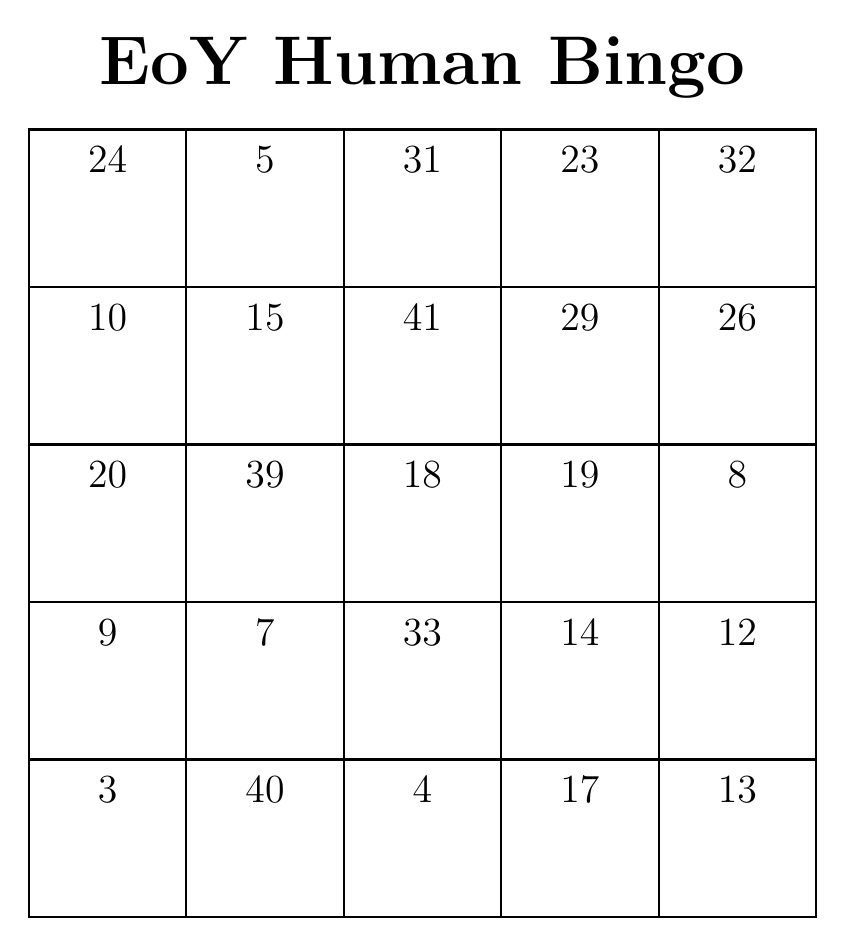
\begin{tikzpicture}
% Set the grid dimensions
\def\cellsize{2cm} % Each cell will be 2x2 cm

% Draw the grid and insert the numbers
\draw[thick] (0, 0) rectangle +(2, 2);
\node[anchor=north, font=\Large, align=center] at (1.0, 1.9) {24};
\draw[thick] (2, 0) rectangle +(2, 2);
\node[anchor=north, font=\Large, align=center] at (3.0, 1.9) {5};
\draw[thick] (4, 0) rectangle +(2, 2);
\node[anchor=north, font=\Large, align=center] at (5.0, 1.9) {31};
\draw[thick] (6, 0) rectangle +(2, 2);
\node[anchor=north, font=\Large, align=center] at (7.0, 1.9) {23};
\draw[thick] (8, 0) rectangle +(2, 2);
\node[anchor=north, font=\Large, align=center] at (9.0, 1.9) {32};
\draw[thick] (0, -2) rectangle +(2, 2);
\node[anchor=north, font=\Large, align=center] at (1.0, -0.1) {10};
\draw[thick] (2, -2) rectangle +(2, 2);
\node[anchor=north, font=\Large, align=center] at (3.0, -0.1) {15};
\draw[thick] (4, -2) rectangle +(2, 2);
\node[anchor=north, font=\Large, align=center] at (5.0, -0.1) {41};
\draw[thick] (6, -2) rectangle +(2, 2);
\node[anchor=north, font=\Large, align=center] at (7.0, -0.1) {29};
\draw[thick] (8, -2) rectangle +(2, 2);
\node[anchor=north, font=\Large, align=center] at (9.0, -0.1) {26};
\draw[thick] (0, -4) rectangle +(2, 2);
\node[anchor=north, font=\Large, align=center] at (1.0, -2.1) {20};
\draw[thick] (2, -4) rectangle +(2, 2);
\node[anchor=north, font=\Large, align=center] at (3.0, -2.1) {39};
\draw[thick] (4, -4) rectangle +(2, 2);
\node[anchor=north, font=\Large, align=center] at (5.0, -2.1) {18};
\draw[thick] (6, -4) rectangle +(2, 2);
\node[anchor=north, font=\Large, align=center] at (7.0, -2.1) {19};
\draw[thick] (8, -4) rectangle +(2, 2);
\node[anchor=north, font=\Large, align=center] at (9.0, -2.1) {8};
\draw[thick] (0, -6) rectangle +(2, 2);
\node[anchor=north, font=\Large, align=center] at (1.0, -4.1) {9};
\draw[thick] (2, -6) rectangle +(2, 2);
\node[anchor=north, font=\Large, align=center] at (3.0, -4.1) {7};
\draw[thick] (4, -6) rectangle +(2, 2);
\node[anchor=north, font=\Large, align=center] at (5.0, -4.1) {33};
\draw[thick] (6, -6) rectangle +(2, 2);
\node[anchor=north, font=\Large, align=center] at (7.0, -4.1) {14};
\draw[thick] (8, -6) rectangle +(2, 2);
\node[anchor=north, font=\Large, align=center] at (9.0, -4.1) {12};
\draw[thick] (0, -8) rectangle +(2, 2);
\node[anchor=north, font=\Large, align=center] at (1.0, -6.1) {3};
\draw[thick] (2, -8) rectangle +(2, 2);
\node[anchor=north, font=\Large, align=center] at (3.0, -6.1) {40};
\draw[thick] (4, -8) rectangle +(2, 2);
\node[anchor=north, font=\Large, align=center] at (5.0, -6.1) {4};
\draw[thick] (6, -8) rectangle +(2, 2);
\node[anchor=north, font=\Large, align=center] at (7.0, -6.1) {17};
\draw[thick] (8, -8) rectangle +(2, 2);
\node[anchor=north, font=\Large, align=center] at (9.0, -6.1) {13};
\node[anchor=north, font = \Huge] at (5.0, 3.3){\textbf{EoY Human Bingo}};
\end{tikzpicture}
\end{center}
\newpage\begin{center}
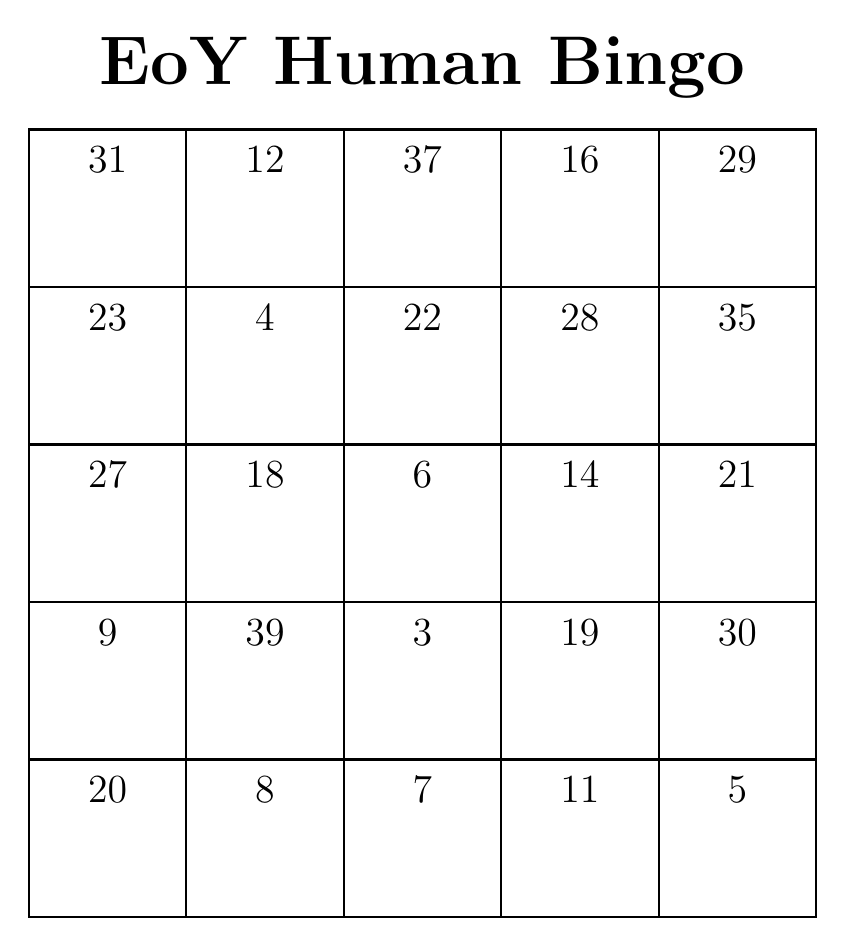
\begin{tikzpicture}
% Set the grid dimensions
\def\cellsize{2cm} % Each cell will be 2x2 cm

% Draw the grid and insert the numbers
\draw[thick] (0, 0) rectangle +(2, 2);
\node[anchor=north, font=\Large, align=center] at (1.0, 1.9) {31};
\draw[thick] (2, 0) rectangle +(2, 2);
\node[anchor=north, font=\Large, align=center] at (3.0, 1.9) {12};
\draw[thick] (4, 0) rectangle +(2, 2);
\node[anchor=north, font=\Large, align=center] at (5.0, 1.9) {37};
\draw[thick] (6, 0) rectangle +(2, 2);
\node[anchor=north, font=\Large, align=center] at (7.0, 1.9) {16};
\draw[thick] (8, 0) rectangle +(2, 2);
\node[anchor=north, font=\Large, align=center] at (9.0, 1.9) {29};
\draw[thick] (0, -2) rectangle +(2, 2);
\node[anchor=north, font=\Large, align=center] at (1.0, -0.1) {23};
\draw[thick] (2, -2) rectangle +(2, 2);
\node[anchor=north, font=\Large, align=center] at (3.0, -0.1) {4};
\draw[thick] (4, -2) rectangle +(2, 2);
\node[anchor=north, font=\Large, align=center] at (5.0, -0.1) {22};
\draw[thick] (6, -2) rectangle +(2, 2);
\node[anchor=north, font=\Large, align=center] at (7.0, -0.1) {28};
\draw[thick] (8, -2) rectangle +(2, 2);
\node[anchor=north, font=\Large, align=center] at (9.0, -0.1) {35};
\draw[thick] (0, -4) rectangle +(2, 2);
\node[anchor=north, font=\Large, align=center] at (1.0, -2.1) {27};
\draw[thick] (2, -4) rectangle +(2, 2);
\node[anchor=north, font=\Large, align=center] at (3.0, -2.1) {18};
\draw[thick] (4, -4) rectangle +(2, 2);
\node[anchor=north, font=\Large, align=center] at (5.0, -2.1) {6};
\draw[thick] (6, -4) rectangle +(2, 2);
\node[anchor=north, font=\Large, align=center] at (7.0, -2.1) {14};
\draw[thick] (8, -4) rectangle +(2, 2);
\node[anchor=north, font=\Large, align=center] at (9.0, -2.1) {21};
\draw[thick] (0, -6) rectangle +(2, 2);
\node[anchor=north, font=\Large, align=center] at (1.0, -4.1) {9};
\draw[thick] (2, -6) rectangle +(2, 2);
\node[anchor=north, font=\Large, align=center] at (3.0, -4.1) {39};
\draw[thick] (4, -6) rectangle +(2, 2);
\node[anchor=north, font=\Large, align=center] at (5.0, -4.1) {3};
\draw[thick] (6, -6) rectangle +(2, 2);
\node[anchor=north, font=\Large, align=center] at (7.0, -4.1) {19};
\draw[thick] (8, -6) rectangle +(2, 2);
\node[anchor=north, font=\Large, align=center] at (9.0, -4.1) {30};
\draw[thick] (0, -8) rectangle +(2, 2);
\node[anchor=north, font=\Large, align=center] at (1.0, -6.1) {20};
\draw[thick] (2, -8) rectangle +(2, 2);
\node[anchor=north, font=\Large, align=center] at (3.0, -6.1) {8};
\draw[thick] (4, -8) rectangle +(2, 2);
\node[anchor=north, font=\Large, align=center] at (5.0, -6.1) {7};
\draw[thick] (6, -8) rectangle +(2, 2);
\node[anchor=north, font=\Large, align=center] at (7.0, -6.1) {11};
\draw[thick] (8, -8) rectangle +(2, 2);
\node[anchor=north, font=\Large, align=center] at (9.0, -6.1) {5};
\node[anchor=north, font = \Huge] at (5.0, 3.3){\textbf{EoY Human Bingo}};
\end{tikzpicture}
\end{center}
\newpage\begin{center}
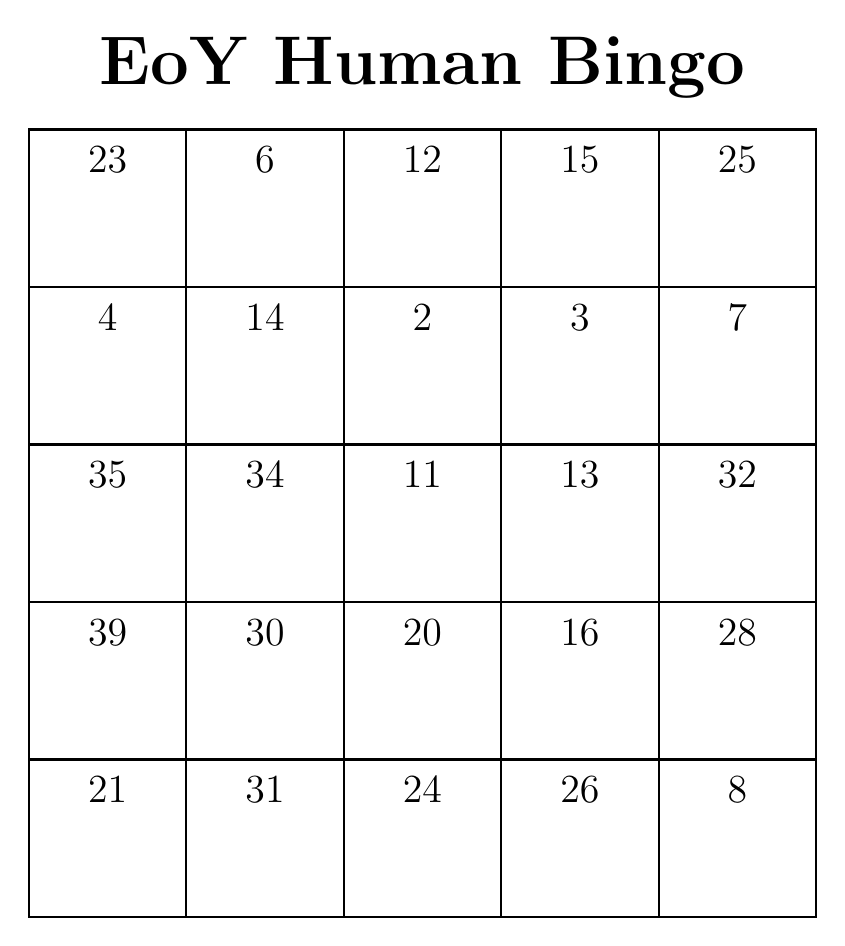
\begin{tikzpicture}
% Set the grid dimensions
\def\cellsize{2cm} % Each cell will be 2x2 cm

% Draw the grid and insert the numbers
\draw[thick] (0, 0) rectangle +(2, 2);
\node[anchor=north, font=\Large, align=center] at (1.0, 1.9) {23};
\draw[thick] (2, 0) rectangle +(2, 2);
\node[anchor=north, font=\Large, align=center] at (3.0, 1.9) {6};
\draw[thick] (4, 0) rectangle +(2, 2);
\node[anchor=north, font=\Large, align=center] at (5.0, 1.9) {12};
\draw[thick] (6, 0) rectangle +(2, 2);
\node[anchor=north, font=\Large, align=center] at (7.0, 1.9) {15};
\draw[thick] (8, 0) rectangle +(2, 2);
\node[anchor=north, font=\Large, align=center] at (9.0, 1.9) {25};
\draw[thick] (0, -2) rectangle +(2, 2);
\node[anchor=north, font=\Large, align=center] at (1.0, -0.1) {4};
\draw[thick] (2, -2) rectangle +(2, 2);
\node[anchor=north, font=\Large, align=center] at (3.0, -0.1) {14};
\draw[thick] (4, -2) rectangle +(2, 2);
\node[anchor=north, font=\Large, align=center] at (5.0, -0.1) {2};
\draw[thick] (6, -2) rectangle +(2, 2);
\node[anchor=north, font=\Large, align=center] at (7.0, -0.1) {3};
\draw[thick] (8, -2) rectangle +(2, 2);
\node[anchor=north, font=\Large, align=center] at (9.0, -0.1) {7};
\draw[thick] (0, -4) rectangle +(2, 2);
\node[anchor=north, font=\Large, align=center] at (1.0, -2.1) {35};
\draw[thick] (2, -4) rectangle +(2, 2);
\node[anchor=north, font=\Large, align=center] at (3.0, -2.1) {34};
\draw[thick] (4, -4) rectangle +(2, 2);
\node[anchor=north, font=\Large, align=center] at (5.0, -2.1) {11};
\draw[thick] (6, -4) rectangle +(2, 2);
\node[anchor=north, font=\Large, align=center] at (7.0, -2.1) {13};
\draw[thick] (8, -4) rectangle +(2, 2);
\node[anchor=north, font=\Large, align=center] at (9.0, -2.1) {32};
\draw[thick] (0, -6) rectangle +(2, 2);
\node[anchor=north, font=\Large, align=center] at (1.0, -4.1) {39};
\draw[thick] (2, -6) rectangle +(2, 2);
\node[anchor=north, font=\Large, align=center] at (3.0, -4.1) {30};
\draw[thick] (4, -6) rectangle +(2, 2);
\node[anchor=north, font=\Large, align=center] at (5.0, -4.1) {20};
\draw[thick] (6, -6) rectangle +(2, 2);
\node[anchor=north, font=\Large, align=center] at (7.0, -4.1) {16};
\draw[thick] (8, -6) rectangle +(2, 2);
\node[anchor=north, font=\Large, align=center] at (9.0, -4.1) {28};
\draw[thick] (0, -8) rectangle +(2, 2);
\node[anchor=north, font=\Large, align=center] at (1.0, -6.1) {21};
\draw[thick] (2, -8) rectangle +(2, 2);
\node[anchor=north, font=\Large, align=center] at (3.0, -6.1) {31};
\draw[thick] (4, -8) rectangle +(2, 2);
\node[anchor=north, font=\Large, align=center] at (5.0, -6.1) {24};
\draw[thick] (6, -8) rectangle +(2, 2);
\node[anchor=north, font=\Large, align=center] at (7.0, -6.1) {26};
\draw[thick] (8, -8) rectangle +(2, 2);
\node[anchor=north, font=\Large, align=center] at (9.0, -6.1) {8};
\node[anchor=north, font = \Huge] at (5.0, 3.3){\textbf{EoY Human Bingo}};
\end{tikzpicture}
\end{center}
\newpage\begin{center}
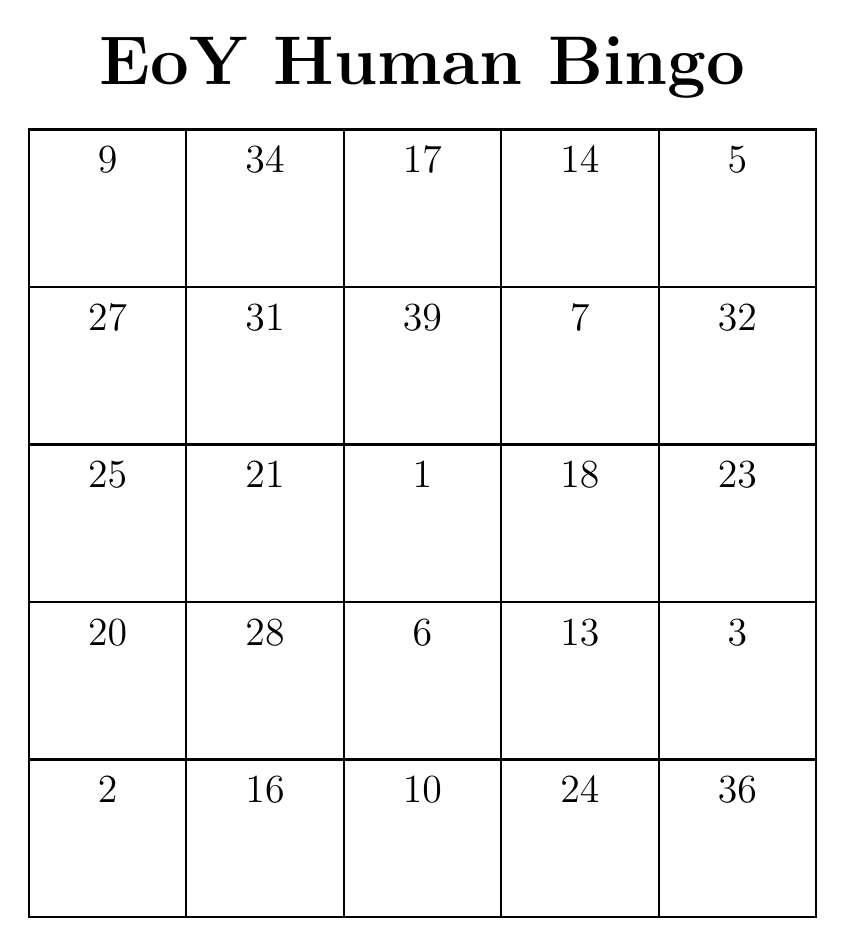
\begin{tikzpicture}
% Set the grid dimensions
\def\cellsize{2cm} % Each cell will be 2x2 cm

% Draw the grid and insert the numbers
\draw[thick] (0, 0) rectangle +(2, 2);
\node[anchor=north, font=\Large, align=center] at (1.0, 1.9) {9};
\draw[thick] (2, 0) rectangle +(2, 2);
\node[anchor=north, font=\Large, align=center] at (3.0, 1.9) {34};
\draw[thick] (4, 0) rectangle +(2, 2);
\node[anchor=north, font=\Large, align=center] at (5.0, 1.9) {17};
\draw[thick] (6, 0) rectangle +(2, 2);
\node[anchor=north, font=\Large, align=center] at (7.0, 1.9) {14};
\draw[thick] (8, 0) rectangle +(2, 2);
\node[anchor=north, font=\Large, align=center] at (9.0, 1.9) {5};
\draw[thick] (0, -2) rectangle +(2, 2);
\node[anchor=north, font=\Large, align=center] at (1.0, -0.1) {27};
\draw[thick] (2, -2) rectangle +(2, 2);
\node[anchor=north, font=\Large, align=center] at (3.0, -0.1) {31};
\draw[thick] (4, -2) rectangle +(2, 2);
\node[anchor=north, font=\Large, align=center] at (5.0, -0.1) {39};
\draw[thick] (6, -2) rectangle +(2, 2);
\node[anchor=north, font=\Large, align=center] at (7.0, -0.1) {7};
\draw[thick] (8, -2) rectangle +(2, 2);
\node[anchor=north, font=\Large, align=center] at (9.0, -0.1) {32};
\draw[thick] (0, -4) rectangle +(2, 2);
\node[anchor=north, font=\Large, align=center] at (1.0, -2.1) {25};
\draw[thick] (2, -4) rectangle +(2, 2);
\node[anchor=north, font=\Large, align=center] at (3.0, -2.1) {21};
\draw[thick] (4, -4) rectangle +(2, 2);
\node[anchor=north, font=\Large, align=center] at (5.0, -2.1) {1};
\draw[thick] (6, -4) rectangle +(2, 2);
\node[anchor=north, font=\Large, align=center] at (7.0, -2.1) {18};
\draw[thick] (8, -4) rectangle +(2, 2);
\node[anchor=north, font=\Large, align=center] at (9.0, -2.1) {23};
\draw[thick] (0, -6) rectangle +(2, 2);
\node[anchor=north, font=\Large, align=center] at (1.0, -4.1) {20};
\draw[thick] (2, -6) rectangle +(2, 2);
\node[anchor=north, font=\Large, align=center] at (3.0, -4.1) {28};
\draw[thick] (4, -6) rectangle +(2, 2);
\node[anchor=north, font=\Large, align=center] at (5.0, -4.1) {6};
\draw[thick] (6, -6) rectangle +(2, 2);
\node[anchor=north, font=\Large, align=center] at (7.0, -4.1) {13};
\draw[thick] (8, -6) rectangle +(2, 2);
\node[anchor=north, font=\Large, align=center] at (9.0, -4.1) {3};
\draw[thick] (0, -8) rectangle +(2, 2);
\node[anchor=north, font=\Large, align=center] at (1.0, -6.1) {2};
\draw[thick] (2, -8) rectangle +(2, 2);
\node[anchor=north, font=\Large, align=center] at (3.0, -6.1) {16};
\draw[thick] (4, -8) rectangle +(2, 2);
\node[anchor=north, font=\Large, align=center] at (5.0, -6.1) {10};
\draw[thick] (6, -8) rectangle +(2, 2);
\node[anchor=north, font=\Large, align=center] at (7.0, -6.1) {24};
\draw[thick] (8, -8) rectangle +(2, 2);
\node[anchor=north, font=\Large, align=center] at (9.0, -6.1) {36};
\node[anchor=north, font = \Huge] at (5.0, 3.3){\textbf{EoY Human Bingo}};
\end{tikzpicture}
\end{center}
\newpage\begin{center}
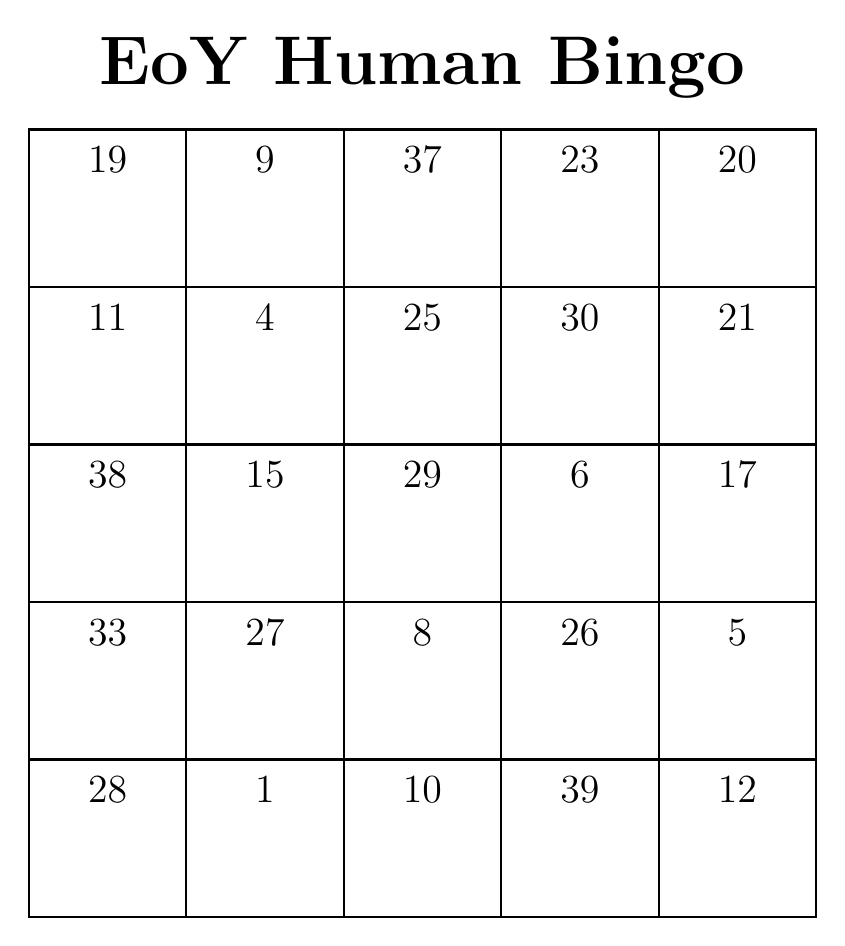
\begin{tikzpicture}
% Set the grid dimensions
\def\cellsize{2cm} % Each cell will be 2x2 cm

% Draw the grid and insert the numbers
\draw[thick] (0, 0) rectangle +(2, 2);
\node[anchor=north, font=\Large, align=center] at (1.0, 1.9) {19};
\draw[thick] (2, 0) rectangle +(2, 2);
\node[anchor=north, font=\Large, align=center] at (3.0, 1.9) {9};
\draw[thick] (4, 0) rectangle +(2, 2);
\node[anchor=north, font=\Large, align=center] at (5.0, 1.9) {37};
\draw[thick] (6, 0) rectangle +(2, 2);
\node[anchor=north, font=\Large, align=center] at (7.0, 1.9) {23};
\draw[thick] (8, 0) rectangle +(2, 2);
\node[anchor=north, font=\Large, align=center] at (9.0, 1.9) {20};
\draw[thick] (0, -2) rectangle +(2, 2);
\node[anchor=north, font=\Large, align=center] at (1.0, -0.1) {11};
\draw[thick] (2, -2) rectangle +(2, 2);
\node[anchor=north, font=\Large, align=center] at (3.0, -0.1) {4};
\draw[thick] (4, -2) rectangle +(2, 2);
\node[anchor=north, font=\Large, align=center] at (5.0, -0.1) {25};
\draw[thick] (6, -2) rectangle +(2, 2);
\node[anchor=north, font=\Large, align=center] at (7.0, -0.1) {30};
\draw[thick] (8, -2) rectangle +(2, 2);
\node[anchor=north, font=\Large, align=center] at (9.0, -0.1) {21};
\draw[thick] (0, -4) rectangle +(2, 2);
\node[anchor=north, font=\Large, align=center] at (1.0, -2.1) {38};
\draw[thick] (2, -4) rectangle +(2, 2);
\node[anchor=north, font=\Large, align=center] at (3.0, -2.1) {15};
\draw[thick] (4, -4) rectangle +(2, 2);
\node[anchor=north, font=\Large, align=center] at (5.0, -2.1) {29};
\draw[thick] (6, -4) rectangle +(2, 2);
\node[anchor=north, font=\Large, align=center] at (7.0, -2.1) {6};
\draw[thick] (8, -4) rectangle +(2, 2);
\node[anchor=north, font=\Large, align=center] at (9.0, -2.1) {17};
\draw[thick] (0, -6) rectangle +(2, 2);
\node[anchor=north, font=\Large, align=center] at (1.0, -4.1) {33};
\draw[thick] (2, -6) rectangle +(2, 2);
\node[anchor=north, font=\Large, align=center] at (3.0, -4.1) {27};
\draw[thick] (4, -6) rectangle +(2, 2);
\node[anchor=north, font=\Large, align=center] at (5.0, -4.1) {8};
\draw[thick] (6, -6) rectangle +(2, 2);
\node[anchor=north, font=\Large, align=center] at (7.0, -4.1) {26};
\draw[thick] (8, -6) rectangle +(2, 2);
\node[anchor=north, font=\Large, align=center] at (9.0, -4.1) {5};
\draw[thick] (0, -8) rectangle +(2, 2);
\node[anchor=north, font=\Large, align=center] at (1.0, -6.1) {28};
\draw[thick] (2, -8) rectangle +(2, 2);
\node[anchor=north, font=\Large, align=center] at (3.0, -6.1) {1};
\draw[thick] (4, -8) rectangle +(2, 2);
\node[anchor=north, font=\Large, align=center] at (5.0, -6.1) {10};
\draw[thick] (6, -8) rectangle +(2, 2);
\node[anchor=north, font=\Large, align=center] at (7.0, -6.1) {39};
\draw[thick] (8, -8) rectangle +(2, 2);
\node[anchor=north, font=\Large, align=center] at (9.0, -6.1) {12};
\node[anchor=north, font = \Huge] at (5.0, 3.3){\textbf{EoY Human Bingo}};
\end{tikzpicture}
\end{center}
\newpage\begin{center}
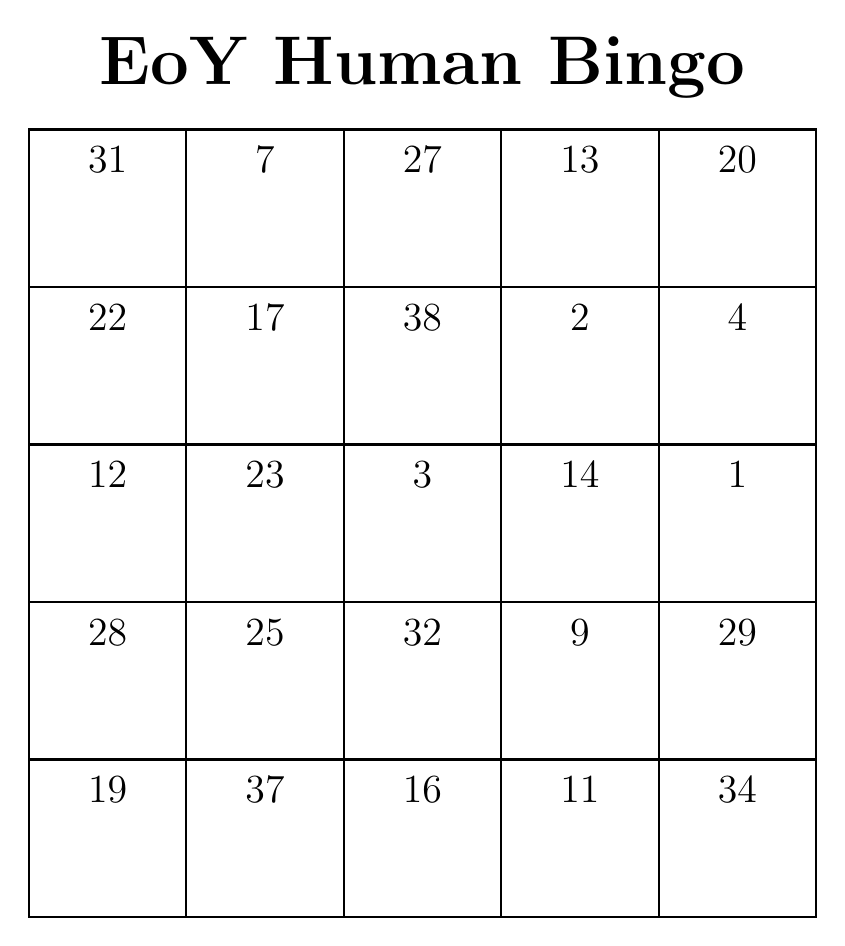
\begin{tikzpicture}
% Set the grid dimensions
\def\cellsize{2cm} % Each cell will be 2x2 cm

% Draw the grid and insert the numbers
\draw[thick] (0, 0) rectangle +(2, 2);
\node[anchor=north, font=\Large, align=center] at (1.0, 1.9) {31};
\draw[thick] (2, 0) rectangle +(2, 2);
\node[anchor=north, font=\Large, align=center] at (3.0, 1.9) {7};
\draw[thick] (4, 0) rectangle +(2, 2);
\node[anchor=north, font=\Large, align=center] at (5.0, 1.9) {27};
\draw[thick] (6, 0) rectangle +(2, 2);
\node[anchor=north, font=\Large, align=center] at (7.0, 1.9) {13};
\draw[thick] (8, 0) rectangle +(2, 2);
\node[anchor=north, font=\Large, align=center] at (9.0, 1.9) {20};
\draw[thick] (0, -2) rectangle +(2, 2);
\node[anchor=north, font=\Large, align=center] at (1.0, -0.1) {22};
\draw[thick] (2, -2) rectangle +(2, 2);
\node[anchor=north, font=\Large, align=center] at (3.0, -0.1) {17};
\draw[thick] (4, -2) rectangle +(2, 2);
\node[anchor=north, font=\Large, align=center] at (5.0, -0.1) {38};
\draw[thick] (6, -2) rectangle +(2, 2);
\node[anchor=north, font=\Large, align=center] at (7.0, -0.1) {2};
\draw[thick] (8, -2) rectangle +(2, 2);
\node[anchor=north, font=\Large, align=center] at (9.0, -0.1) {4};
\draw[thick] (0, -4) rectangle +(2, 2);
\node[anchor=north, font=\Large, align=center] at (1.0, -2.1) {12};
\draw[thick] (2, -4) rectangle +(2, 2);
\node[anchor=north, font=\Large, align=center] at (3.0, -2.1) {23};
\draw[thick] (4, -4) rectangle +(2, 2);
\node[anchor=north, font=\Large, align=center] at (5.0, -2.1) {3};
\draw[thick] (6, -4) rectangle +(2, 2);
\node[anchor=north, font=\Large, align=center] at (7.0, -2.1) {14};
\draw[thick] (8, -4) rectangle +(2, 2);
\node[anchor=north, font=\Large, align=center] at (9.0, -2.1) {1};
\draw[thick] (0, -6) rectangle +(2, 2);
\node[anchor=north, font=\Large, align=center] at (1.0, -4.1) {28};
\draw[thick] (2, -6) rectangle +(2, 2);
\node[anchor=north, font=\Large, align=center] at (3.0, -4.1) {25};
\draw[thick] (4, -6) rectangle +(2, 2);
\node[anchor=north, font=\Large, align=center] at (5.0, -4.1) {32};
\draw[thick] (6, -6) rectangle +(2, 2);
\node[anchor=north, font=\Large, align=center] at (7.0, -4.1) {9};
\draw[thick] (8, -6) rectangle +(2, 2);
\node[anchor=north, font=\Large, align=center] at (9.0, -4.1) {29};
\draw[thick] (0, -8) rectangle +(2, 2);
\node[anchor=north, font=\Large, align=center] at (1.0, -6.1) {19};
\draw[thick] (2, -8) rectangle +(2, 2);
\node[anchor=north, font=\Large, align=center] at (3.0, -6.1) {37};
\draw[thick] (4, -8) rectangle +(2, 2);
\node[anchor=north, font=\Large, align=center] at (5.0, -6.1) {16};
\draw[thick] (6, -8) rectangle +(2, 2);
\node[anchor=north, font=\Large, align=center] at (7.0, -6.1) {11};
\draw[thick] (8, -8) rectangle +(2, 2);
\node[anchor=north, font=\Large, align=center] at (9.0, -6.1) {34};
\node[anchor=north, font = \Huge] at (5.0, 3.3){\textbf{EoY Human Bingo}};
\end{tikzpicture}
\end{center}
\newpage\begin{center}
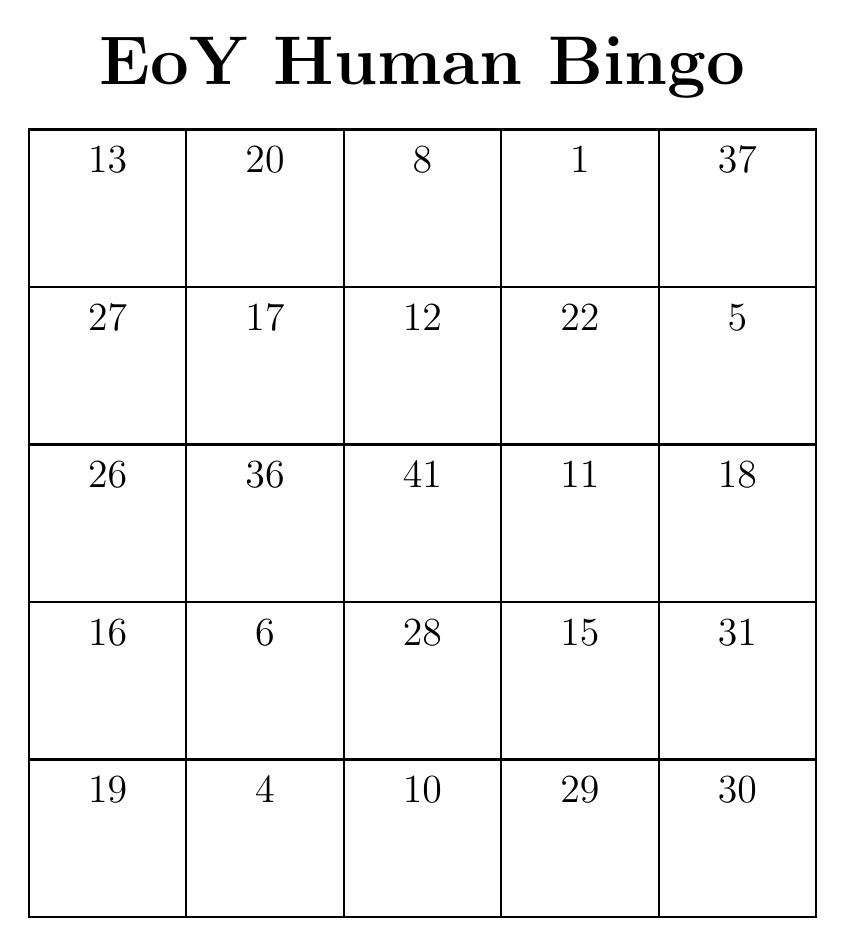
\begin{tikzpicture}
% Set the grid dimensions
\def\cellsize{2cm} % Each cell will be 2x2 cm

% Draw the grid and insert the numbers
\draw[thick] (0, 0) rectangle +(2, 2);
\node[anchor=north, font=\Large, align=center] at (1.0, 1.9) {13};
\draw[thick] (2, 0) rectangle +(2, 2);
\node[anchor=north, font=\Large, align=center] at (3.0, 1.9) {20};
\draw[thick] (4, 0) rectangle +(2, 2);
\node[anchor=north, font=\Large, align=center] at (5.0, 1.9) {8};
\draw[thick] (6, 0) rectangle +(2, 2);
\node[anchor=north, font=\Large, align=center] at (7.0, 1.9) {1};
\draw[thick] (8, 0) rectangle +(2, 2);
\node[anchor=north, font=\Large, align=center] at (9.0, 1.9) {37};
\draw[thick] (0, -2) rectangle +(2, 2);
\node[anchor=north, font=\Large, align=center] at (1.0, -0.1) {27};
\draw[thick] (2, -2) rectangle +(2, 2);
\node[anchor=north, font=\Large, align=center] at (3.0, -0.1) {17};
\draw[thick] (4, -2) rectangle +(2, 2);
\node[anchor=north, font=\Large, align=center] at (5.0, -0.1) {12};
\draw[thick] (6, -2) rectangle +(2, 2);
\node[anchor=north, font=\Large, align=center] at (7.0, -0.1) {22};
\draw[thick] (8, -2) rectangle +(2, 2);
\node[anchor=north, font=\Large, align=center] at (9.0, -0.1) {5};
\draw[thick] (0, -4) rectangle +(2, 2);
\node[anchor=north, font=\Large, align=center] at (1.0, -2.1) {26};
\draw[thick] (2, -4) rectangle +(2, 2);
\node[anchor=north, font=\Large, align=center] at (3.0, -2.1) {36};
\draw[thick] (4, -4) rectangle +(2, 2);
\node[anchor=north, font=\Large, align=center] at (5.0, -2.1) {41};
\draw[thick] (6, -4) rectangle +(2, 2);
\node[anchor=north, font=\Large, align=center] at (7.0, -2.1) {11};
\draw[thick] (8, -4) rectangle +(2, 2);
\node[anchor=north, font=\Large, align=center] at (9.0, -2.1) {18};
\draw[thick] (0, -6) rectangle +(2, 2);
\node[anchor=north, font=\Large, align=center] at (1.0, -4.1) {16};
\draw[thick] (2, -6) rectangle +(2, 2);
\node[anchor=north, font=\Large, align=center] at (3.0, -4.1) {6};
\draw[thick] (4, -6) rectangle +(2, 2);
\node[anchor=north, font=\Large, align=center] at (5.0, -4.1) {28};
\draw[thick] (6, -6) rectangle +(2, 2);
\node[anchor=north, font=\Large, align=center] at (7.0, -4.1) {15};
\draw[thick] (8, -6) rectangle +(2, 2);
\node[anchor=north, font=\Large, align=center] at (9.0, -4.1) {31};
\draw[thick] (0, -8) rectangle +(2, 2);
\node[anchor=north, font=\Large, align=center] at (1.0, -6.1) {19};
\draw[thick] (2, -8) rectangle +(2, 2);
\node[anchor=north, font=\Large, align=center] at (3.0, -6.1) {4};
\draw[thick] (4, -8) rectangle +(2, 2);
\node[anchor=north, font=\Large, align=center] at (5.0, -6.1) {10};
\draw[thick] (6, -8) rectangle +(2, 2);
\node[anchor=north, font=\Large, align=center] at (7.0, -6.1) {29};
\draw[thick] (8, -8) rectangle +(2, 2);
\node[anchor=north, font=\Large, align=center] at (9.0, -6.1) {30};
\node[anchor=north, font = \Huge] at (5.0, 3.3){\textbf{EoY Human Bingo}};
\end{tikzpicture}
\end{center}
\newpage\begin{center}
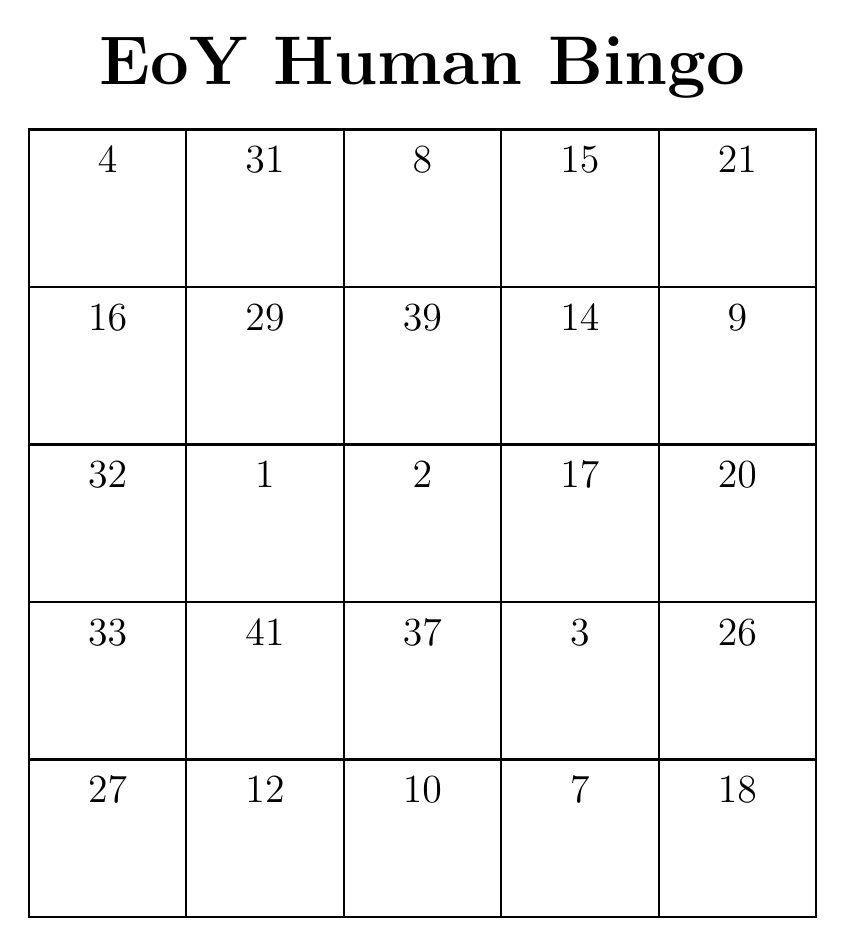
\begin{tikzpicture}
% Set the grid dimensions
\def\cellsize{2cm} % Each cell will be 2x2 cm

% Draw the grid and insert the numbers
\draw[thick] (0, 0) rectangle +(2, 2);
\node[anchor=north, font=\Large, align=center] at (1.0, 1.9) {4};
\draw[thick] (2, 0) rectangle +(2, 2);
\node[anchor=north, font=\Large, align=center] at (3.0, 1.9) {31};
\draw[thick] (4, 0) rectangle +(2, 2);
\node[anchor=north, font=\Large, align=center] at (5.0, 1.9) {8};
\draw[thick] (6, 0) rectangle +(2, 2);
\node[anchor=north, font=\Large, align=center] at (7.0, 1.9) {15};
\draw[thick] (8, 0) rectangle +(2, 2);
\node[anchor=north, font=\Large, align=center] at (9.0, 1.9) {21};
\draw[thick] (0, -2) rectangle +(2, 2);
\node[anchor=north, font=\Large, align=center] at (1.0, -0.1) {16};
\draw[thick] (2, -2) rectangle +(2, 2);
\node[anchor=north, font=\Large, align=center] at (3.0, -0.1) {29};
\draw[thick] (4, -2) rectangle +(2, 2);
\node[anchor=north, font=\Large, align=center] at (5.0, -0.1) {39};
\draw[thick] (6, -2) rectangle +(2, 2);
\node[anchor=north, font=\Large, align=center] at (7.0, -0.1) {14};
\draw[thick] (8, -2) rectangle +(2, 2);
\node[anchor=north, font=\Large, align=center] at (9.0, -0.1) {9};
\draw[thick] (0, -4) rectangle +(2, 2);
\node[anchor=north, font=\Large, align=center] at (1.0, -2.1) {32};
\draw[thick] (2, -4) rectangle +(2, 2);
\node[anchor=north, font=\Large, align=center] at (3.0, -2.1) {1};
\draw[thick] (4, -4) rectangle +(2, 2);
\node[anchor=north, font=\Large, align=center] at (5.0, -2.1) {2};
\draw[thick] (6, -4) rectangle +(2, 2);
\node[anchor=north, font=\Large, align=center] at (7.0, -2.1) {17};
\draw[thick] (8, -4) rectangle +(2, 2);
\node[anchor=north, font=\Large, align=center] at (9.0, -2.1) {20};
\draw[thick] (0, -6) rectangle +(2, 2);
\node[anchor=north, font=\Large, align=center] at (1.0, -4.1) {33};
\draw[thick] (2, -6) rectangle +(2, 2);
\node[anchor=north, font=\Large, align=center] at (3.0, -4.1) {41};
\draw[thick] (4, -6) rectangle +(2, 2);
\node[anchor=north, font=\Large, align=center] at (5.0, -4.1) {37};
\draw[thick] (6, -6) rectangle +(2, 2);
\node[anchor=north, font=\Large, align=center] at (7.0, -4.1) {3};
\draw[thick] (8, -6) rectangle +(2, 2);
\node[anchor=north, font=\Large, align=center] at (9.0, -4.1) {26};
\draw[thick] (0, -8) rectangle +(2, 2);
\node[anchor=north, font=\Large, align=center] at (1.0, -6.1) {27};
\draw[thick] (2, -8) rectangle +(2, 2);
\node[anchor=north, font=\Large, align=center] at (3.0, -6.1) {12};
\draw[thick] (4, -8) rectangle +(2, 2);
\node[anchor=north, font=\Large, align=center] at (5.0, -6.1) {10};
\draw[thick] (6, -8) rectangle +(2, 2);
\node[anchor=north, font=\Large, align=center] at (7.0, -6.1) {7};
\draw[thick] (8, -8) rectangle +(2, 2);
\node[anchor=north, font=\Large, align=center] at (9.0, -6.1) {18};
\node[anchor=north, font = \Huge] at (5.0, 3.3){\textbf{EoY Human Bingo}};
\end{tikzpicture}
\end{center}
\newpage\begin{center}
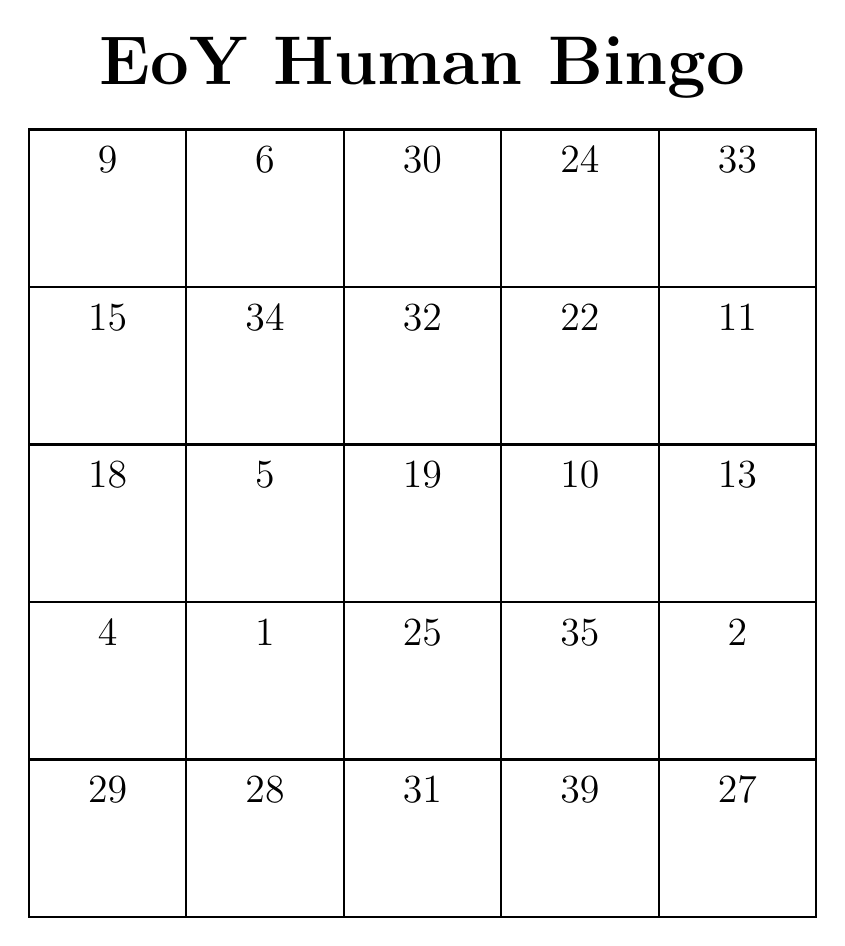
\begin{tikzpicture}
% Set the grid dimensions
\def\cellsize{2cm} % Each cell will be 2x2 cm

% Draw the grid and insert the numbers
\draw[thick] (0, 0) rectangle +(2, 2);
\node[anchor=north, font=\Large, align=center] at (1.0, 1.9) {9};
\draw[thick] (2, 0) rectangle +(2, 2);
\node[anchor=north, font=\Large, align=center] at (3.0, 1.9) {6};
\draw[thick] (4, 0) rectangle +(2, 2);
\node[anchor=north, font=\Large, align=center] at (5.0, 1.9) {30};
\draw[thick] (6, 0) rectangle +(2, 2);
\node[anchor=north, font=\Large, align=center] at (7.0, 1.9) {24};
\draw[thick] (8, 0) rectangle +(2, 2);
\node[anchor=north, font=\Large, align=center] at (9.0, 1.9) {33};
\draw[thick] (0, -2) rectangle +(2, 2);
\node[anchor=north, font=\Large, align=center] at (1.0, -0.1) {15};
\draw[thick] (2, -2) rectangle +(2, 2);
\node[anchor=north, font=\Large, align=center] at (3.0, -0.1) {34};
\draw[thick] (4, -2) rectangle +(2, 2);
\node[anchor=north, font=\Large, align=center] at (5.0, -0.1) {32};
\draw[thick] (6, -2) rectangle +(2, 2);
\node[anchor=north, font=\Large, align=center] at (7.0, -0.1) {22};
\draw[thick] (8, -2) rectangle +(2, 2);
\node[anchor=north, font=\Large, align=center] at (9.0, -0.1) {11};
\draw[thick] (0, -4) rectangle +(2, 2);
\node[anchor=north, font=\Large, align=center] at (1.0, -2.1) {18};
\draw[thick] (2, -4) rectangle +(2, 2);
\node[anchor=north, font=\Large, align=center] at (3.0, -2.1) {5};
\draw[thick] (4, -4) rectangle +(2, 2);
\node[anchor=north, font=\Large, align=center] at (5.0, -2.1) {19};
\draw[thick] (6, -4) rectangle +(2, 2);
\node[anchor=north, font=\Large, align=center] at (7.0, -2.1) {10};
\draw[thick] (8, -4) rectangle +(2, 2);
\node[anchor=north, font=\Large, align=center] at (9.0, -2.1) {13};
\draw[thick] (0, -6) rectangle +(2, 2);
\node[anchor=north, font=\Large, align=center] at (1.0, -4.1) {4};
\draw[thick] (2, -6) rectangle +(2, 2);
\node[anchor=north, font=\Large, align=center] at (3.0, -4.1) {1};
\draw[thick] (4, -6) rectangle +(2, 2);
\node[anchor=north, font=\Large, align=center] at (5.0, -4.1) {25};
\draw[thick] (6, -6) rectangle +(2, 2);
\node[anchor=north, font=\Large, align=center] at (7.0, -4.1) {35};
\draw[thick] (8, -6) rectangle +(2, 2);
\node[anchor=north, font=\Large, align=center] at (9.0, -4.1) {2};
\draw[thick] (0, -8) rectangle +(2, 2);
\node[anchor=north, font=\Large, align=center] at (1.0, -6.1) {29};
\draw[thick] (2, -8) rectangle +(2, 2);
\node[anchor=north, font=\Large, align=center] at (3.0, -6.1) {28};
\draw[thick] (4, -8) rectangle +(2, 2);
\node[anchor=north, font=\Large, align=center] at (5.0, -6.1) {31};
\draw[thick] (6, -8) rectangle +(2, 2);
\node[anchor=north, font=\Large, align=center] at (7.0, -6.1) {39};
\draw[thick] (8, -8) rectangle +(2, 2);
\node[anchor=north, font=\Large, align=center] at (9.0, -6.1) {27};
\node[anchor=north, font = \Huge] at (5.0, 3.3){\textbf{EoY Human Bingo}};
\end{tikzpicture}
\end{center}
\newpage\begin{center}
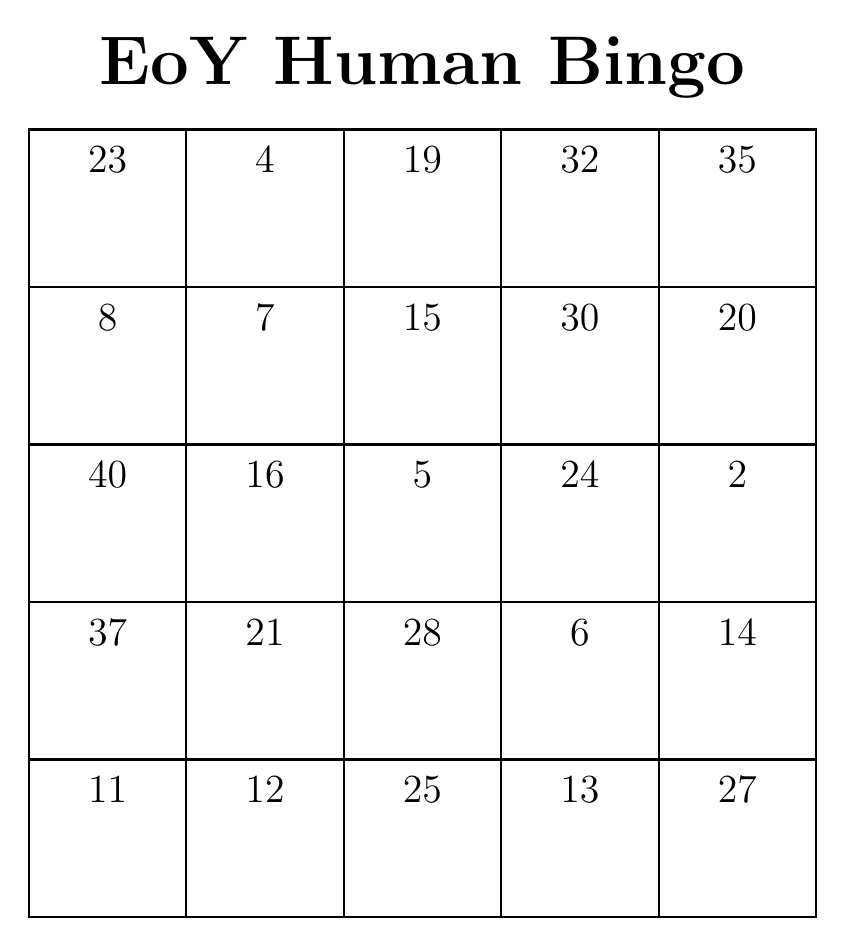
\begin{tikzpicture}
% Set the grid dimensions
\def\cellsize{2cm} % Each cell will be 2x2 cm

% Draw the grid and insert the numbers
\draw[thick] (0, 0) rectangle +(2, 2);
\node[anchor=north, font=\Large, align=center] at (1.0, 1.9) {23};
\draw[thick] (2, 0) rectangle +(2, 2);
\node[anchor=north, font=\Large, align=center] at (3.0, 1.9) {4};
\draw[thick] (4, 0) rectangle +(2, 2);
\node[anchor=north, font=\Large, align=center] at (5.0, 1.9) {19};
\draw[thick] (6, 0) rectangle +(2, 2);
\node[anchor=north, font=\Large, align=center] at (7.0, 1.9) {32};
\draw[thick] (8, 0) rectangle +(2, 2);
\node[anchor=north, font=\Large, align=center] at (9.0, 1.9) {35};
\draw[thick] (0, -2) rectangle +(2, 2);
\node[anchor=north, font=\Large, align=center] at (1.0, -0.1) {8};
\draw[thick] (2, -2) rectangle +(2, 2);
\node[anchor=north, font=\Large, align=center] at (3.0, -0.1) {7};
\draw[thick] (4, -2) rectangle +(2, 2);
\node[anchor=north, font=\Large, align=center] at (5.0, -0.1) {15};
\draw[thick] (6, -2) rectangle +(2, 2);
\node[anchor=north, font=\Large, align=center] at (7.0, -0.1) {30};
\draw[thick] (8, -2) rectangle +(2, 2);
\node[anchor=north, font=\Large, align=center] at (9.0, -0.1) {20};
\draw[thick] (0, -4) rectangle +(2, 2);
\node[anchor=north, font=\Large, align=center] at (1.0, -2.1) {40};
\draw[thick] (2, -4) rectangle +(2, 2);
\node[anchor=north, font=\Large, align=center] at (3.0, -2.1) {16};
\draw[thick] (4, -4) rectangle +(2, 2);
\node[anchor=north, font=\Large, align=center] at (5.0, -2.1) {5};
\draw[thick] (6, -4) rectangle +(2, 2);
\node[anchor=north, font=\Large, align=center] at (7.0, -2.1) {24};
\draw[thick] (8, -4) rectangle +(2, 2);
\node[anchor=north, font=\Large, align=center] at (9.0, -2.1) {2};
\draw[thick] (0, -6) rectangle +(2, 2);
\node[anchor=north, font=\Large, align=center] at (1.0, -4.1) {37};
\draw[thick] (2, -6) rectangle +(2, 2);
\node[anchor=north, font=\Large, align=center] at (3.0, -4.1) {21};
\draw[thick] (4, -6) rectangle +(2, 2);
\node[anchor=north, font=\Large, align=center] at (5.0, -4.1) {28};
\draw[thick] (6, -6) rectangle +(2, 2);
\node[anchor=north, font=\Large, align=center] at (7.0, -4.1) {6};
\draw[thick] (8, -6) rectangle +(2, 2);
\node[anchor=north, font=\Large, align=center] at (9.0, -4.1) {14};
\draw[thick] (0, -8) rectangle +(2, 2);
\node[anchor=north, font=\Large, align=center] at (1.0, -6.1) {11};
\draw[thick] (2, -8) rectangle +(2, 2);
\node[anchor=north, font=\Large, align=center] at (3.0, -6.1) {12};
\draw[thick] (4, -8) rectangle +(2, 2);
\node[anchor=north, font=\Large, align=center] at (5.0, -6.1) {25};
\draw[thick] (6, -8) rectangle +(2, 2);
\node[anchor=north, font=\Large, align=center] at (7.0, -6.1) {13};
\draw[thick] (8, -8) rectangle +(2, 2);
\node[anchor=north, font=\Large, align=center] at (9.0, -6.1) {27};
\node[anchor=north, font = \Huge] at (5.0, 3.3){\textbf{EoY Human Bingo}};
\end{tikzpicture}
\end{center}
\newpage\begin{center}
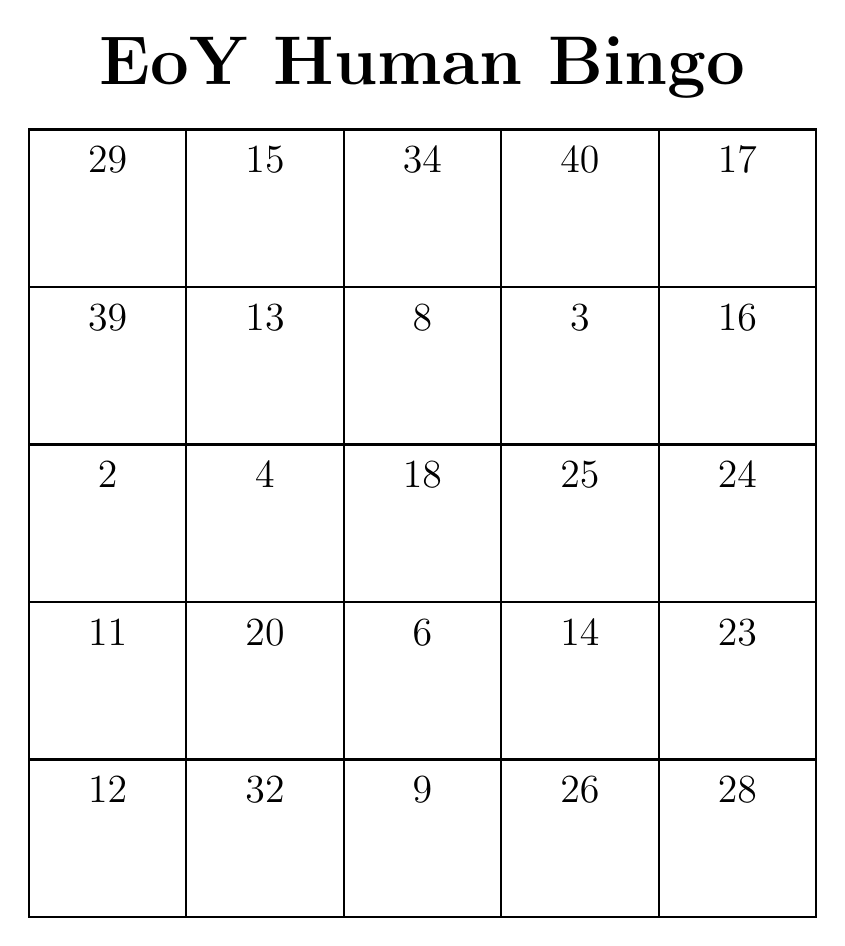
\begin{tikzpicture}
% Set the grid dimensions
\def\cellsize{2cm} % Each cell will be 2x2 cm

% Draw the grid and insert the numbers
\draw[thick] (0, 0) rectangle +(2, 2);
\node[anchor=north, font=\Large, align=center] at (1.0, 1.9) {29};
\draw[thick] (2, 0) rectangle +(2, 2);
\node[anchor=north, font=\Large, align=center] at (3.0, 1.9) {15};
\draw[thick] (4, 0) rectangle +(2, 2);
\node[anchor=north, font=\Large, align=center] at (5.0, 1.9) {34};
\draw[thick] (6, 0) rectangle +(2, 2);
\node[anchor=north, font=\Large, align=center] at (7.0, 1.9) {40};
\draw[thick] (8, 0) rectangle +(2, 2);
\node[anchor=north, font=\Large, align=center] at (9.0, 1.9) {17};
\draw[thick] (0, -2) rectangle +(2, 2);
\node[anchor=north, font=\Large, align=center] at (1.0, -0.1) {39};
\draw[thick] (2, -2) rectangle +(2, 2);
\node[anchor=north, font=\Large, align=center] at (3.0, -0.1) {13};
\draw[thick] (4, -2) rectangle +(2, 2);
\node[anchor=north, font=\Large, align=center] at (5.0, -0.1) {8};
\draw[thick] (6, -2) rectangle +(2, 2);
\node[anchor=north, font=\Large, align=center] at (7.0, -0.1) {3};
\draw[thick] (8, -2) rectangle +(2, 2);
\node[anchor=north, font=\Large, align=center] at (9.0, -0.1) {16};
\draw[thick] (0, -4) rectangle +(2, 2);
\node[anchor=north, font=\Large, align=center] at (1.0, -2.1) {2};
\draw[thick] (2, -4) rectangle +(2, 2);
\node[anchor=north, font=\Large, align=center] at (3.0, -2.1) {4};
\draw[thick] (4, -4) rectangle +(2, 2);
\node[anchor=north, font=\Large, align=center] at (5.0, -2.1) {18};
\draw[thick] (6, -4) rectangle +(2, 2);
\node[anchor=north, font=\Large, align=center] at (7.0, -2.1) {25};
\draw[thick] (8, -4) rectangle +(2, 2);
\node[anchor=north, font=\Large, align=center] at (9.0, -2.1) {24};
\draw[thick] (0, -6) rectangle +(2, 2);
\node[anchor=north, font=\Large, align=center] at (1.0, -4.1) {11};
\draw[thick] (2, -6) rectangle +(2, 2);
\node[anchor=north, font=\Large, align=center] at (3.0, -4.1) {20};
\draw[thick] (4, -6) rectangle +(2, 2);
\node[anchor=north, font=\Large, align=center] at (5.0, -4.1) {6};
\draw[thick] (6, -6) rectangle +(2, 2);
\node[anchor=north, font=\Large, align=center] at (7.0, -4.1) {14};
\draw[thick] (8, -6) rectangle +(2, 2);
\node[anchor=north, font=\Large, align=center] at (9.0, -4.1) {23};
\draw[thick] (0, -8) rectangle +(2, 2);
\node[anchor=north, font=\Large, align=center] at (1.0, -6.1) {12};
\draw[thick] (2, -8) rectangle +(2, 2);
\node[anchor=north, font=\Large, align=center] at (3.0, -6.1) {32};
\draw[thick] (4, -8) rectangle +(2, 2);
\node[anchor=north, font=\Large, align=center] at (5.0, -6.1) {9};
\draw[thick] (6, -8) rectangle +(2, 2);
\node[anchor=north, font=\Large, align=center] at (7.0, -6.1) {26};
\draw[thick] (8, -8) rectangle +(2, 2);
\node[anchor=north, font=\Large, align=center] at (9.0, -6.1) {28};
\node[anchor=north, font = \Huge] at (5.0, 3.3){\textbf{EoY Human Bingo}};
\end{tikzpicture}
\end{center}
\newpage\begin{center}
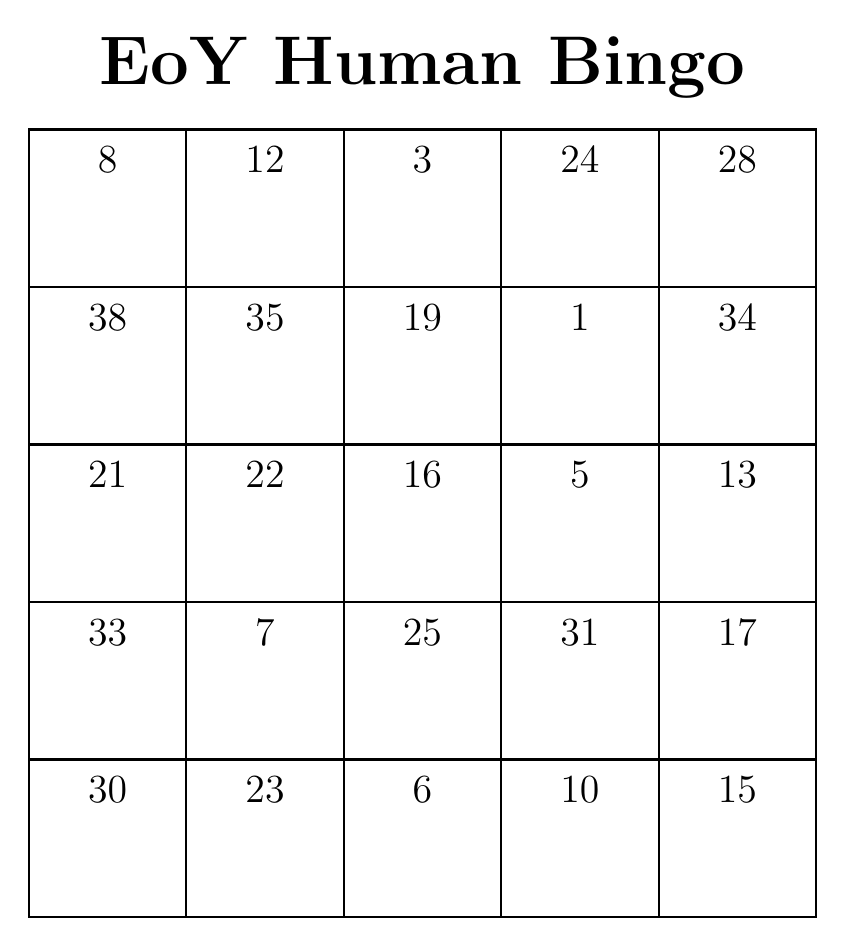
\begin{tikzpicture}
% Set the grid dimensions
\def\cellsize{2cm} % Each cell will be 2x2 cm

% Draw the grid and insert the numbers
\draw[thick] (0, 0) rectangle +(2, 2);
\node[anchor=north, font=\Large, align=center] at (1.0, 1.9) {8};
\draw[thick] (2, 0) rectangle +(2, 2);
\node[anchor=north, font=\Large, align=center] at (3.0, 1.9) {12};
\draw[thick] (4, 0) rectangle +(2, 2);
\node[anchor=north, font=\Large, align=center] at (5.0, 1.9) {3};
\draw[thick] (6, 0) rectangle +(2, 2);
\node[anchor=north, font=\Large, align=center] at (7.0, 1.9) {24};
\draw[thick] (8, 0) rectangle +(2, 2);
\node[anchor=north, font=\Large, align=center] at (9.0, 1.9) {28};
\draw[thick] (0, -2) rectangle +(2, 2);
\node[anchor=north, font=\Large, align=center] at (1.0, -0.1) {38};
\draw[thick] (2, -2) rectangle +(2, 2);
\node[anchor=north, font=\Large, align=center] at (3.0, -0.1) {35};
\draw[thick] (4, -2) rectangle +(2, 2);
\node[anchor=north, font=\Large, align=center] at (5.0, -0.1) {19};
\draw[thick] (6, -2) rectangle +(2, 2);
\node[anchor=north, font=\Large, align=center] at (7.0, -0.1) {1};
\draw[thick] (8, -2) rectangle +(2, 2);
\node[anchor=north, font=\Large, align=center] at (9.0, -0.1) {34};
\draw[thick] (0, -4) rectangle +(2, 2);
\node[anchor=north, font=\Large, align=center] at (1.0, -2.1) {21};
\draw[thick] (2, -4) rectangle +(2, 2);
\node[anchor=north, font=\Large, align=center] at (3.0, -2.1) {22};
\draw[thick] (4, -4) rectangle +(2, 2);
\node[anchor=north, font=\Large, align=center] at (5.0, -2.1) {16};
\draw[thick] (6, -4) rectangle +(2, 2);
\node[anchor=north, font=\Large, align=center] at (7.0, -2.1) {5};
\draw[thick] (8, -4) rectangle +(2, 2);
\node[anchor=north, font=\Large, align=center] at (9.0, -2.1) {13};
\draw[thick] (0, -6) rectangle +(2, 2);
\node[anchor=north, font=\Large, align=center] at (1.0, -4.1) {33};
\draw[thick] (2, -6) rectangle +(2, 2);
\node[anchor=north, font=\Large, align=center] at (3.0, -4.1) {7};
\draw[thick] (4, -6) rectangle +(2, 2);
\node[anchor=north, font=\Large, align=center] at (5.0, -4.1) {25};
\draw[thick] (6, -6) rectangle +(2, 2);
\node[anchor=north, font=\Large, align=center] at (7.0, -4.1) {31};
\draw[thick] (8, -6) rectangle +(2, 2);
\node[anchor=north, font=\Large, align=center] at (9.0, -4.1) {17};
\draw[thick] (0, -8) rectangle +(2, 2);
\node[anchor=north, font=\Large, align=center] at (1.0, -6.1) {30};
\draw[thick] (2, -8) rectangle +(2, 2);
\node[anchor=north, font=\Large, align=center] at (3.0, -6.1) {23};
\draw[thick] (4, -8) rectangle +(2, 2);
\node[anchor=north, font=\Large, align=center] at (5.0, -6.1) {6};
\draw[thick] (6, -8) rectangle +(2, 2);
\node[anchor=north, font=\Large, align=center] at (7.0, -6.1) {10};
\draw[thick] (8, -8) rectangle +(2, 2);
\node[anchor=north, font=\Large, align=center] at (9.0, -6.1) {15};
\node[anchor=north, font = \Huge] at (5.0, 3.3){\textbf{EoY Human Bingo}};
\end{tikzpicture}
\end{center}
\newpage\begin{center}
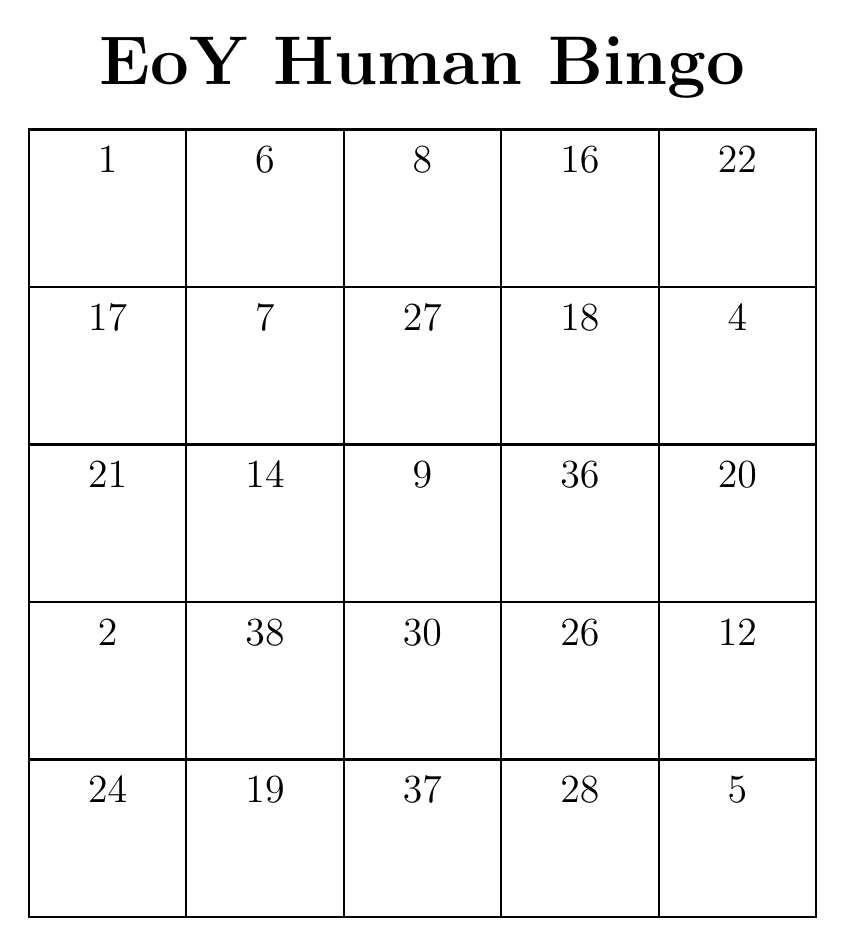
\begin{tikzpicture}
% Set the grid dimensions
\def\cellsize{2cm} % Each cell will be 2x2 cm

% Draw the grid and insert the numbers
\draw[thick] (0, 0) rectangle +(2, 2);
\node[anchor=north, font=\Large, align=center] at (1.0, 1.9) {1};
\draw[thick] (2, 0) rectangle +(2, 2);
\node[anchor=north, font=\Large, align=center] at (3.0, 1.9) {6};
\draw[thick] (4, 0) rectangle +(2, 2);
\node[anchor=north, font=\Large, align=center] at (5.0, 1.9) {8};
\draw[thick] (6, 0) rectangle +(2, 2);
\node[anchor=north, font=\Large, align=center] at (7.0, 1.9) {16};
\draw[thick] (8, 0) rectangle +(2, 2);
\node[anchor=north, font=\Large, align=center] at (9.0, 1.9) {22};
\draw[thick] (0, -2) rectangle +(2, 2);
\node[anchor=north, font=\Large, align=center] at (1.0, -0.1) {17};
\draw[thick] (2, -2) rectangle +(2, 2);
\node[anchor=north, font=\Large, align=center] at (3.0, -0.1) {7};
\draw[thick] (4, -2) rectangle +(2, 2);
\node[anchor=north, font=\Large, align=center] at (5.0, -0.1) {27};
\draw[thick] (6, -2) rectangle +(2, 2);
\node[anchor=north, font=\Large, align=center] at (7.0, -0.1) {18};
\draw[thick] (8, -2) rectangle +(2, 2);
\node[anchor=north, font=\Large, align=center] at (9.0, -0.1) {4};
\draw[thick] (0, -4) rectangle +(2, 2);
\node[anchor=north, font=\Large, align=center] at (1.0, -2.1) {21};
\draw[thick] (2, -4) rectangle +(2, 2);
\node[anchor=north, font=\Large, align=center] at (3.0, -2.1) {14};
\draw[thick] (4, -4) rectangle +(2, 2);
\node[anchor=north, font=\Large, align=center] at (5.0, -2.1) {9};
\draw[thick] (6, -4) rectangle +(2, 2);
\node[anchor=north, font=\Large, align=center] at (7.0, -2.1) {36};
\draw[thick] (8, -4) rectangle +(2, 2);
\node[anchor=north, font=\Large, align=center] at (9.0, -2.1) {20};
\draw[thick] (0, -6) rectangle +(2, 2);
\node[anchor=north, font=\Large, align=center] at (1.0, -4.1) {2};
\draw[thick] (2, -6) rectangle +(2, 2);
\node[anchor=north, font=\Large, align=center] at (3.0, -4.1) {38};
\draw[thick] (4, -6) rectangle +(2, 2);
\node[anchor=north, font=\Large, align=center] at (5.0, -4.1) {30};
\draw[thick] (6, -6) rectangle +(2, 2);
\node[anchor=north, font=\Large, align=center] at (7.0, -4.1) {26};
\draw[thick] (8, -6) rectangle +(2, 2);
\node[anchor=north, font=\Large, align=center] at (9.0, -4.1) {12};
\draw[thick] (0, -8) rectangle +(2, 2);
\node[anchor=north, font=\Large, align=center] at (1.0, -6.1) {24};
\draw[thick] (2, -8) rectangle +(2, 2);
\node[anchor=north, font=\Large, align=center] at (3.0, -6.1) {19};
\draw[thick] (4, -8) rectangle +(2, 2);
\node[anchor=north, font=\Large, align=center] at (5.0, -6.1) {37};
\draw[thick] (6, -8) rectangle +(2, 2);
\node[anchor=north, font=\Large, align=center] at (7.0, -6.1) {28};
\draw[thick] (8, -8) rectangle +(2, 2);
\node[anchor=north, font=\Large, align=center] at (9.0, -6.1) {5};
\node[anchor=north, font = \Huge] at (5.0, 3.3){\textbf{EoY Human Bingo}};
\end{tikzpicture}
\end{center}
\newpage\begin{center}
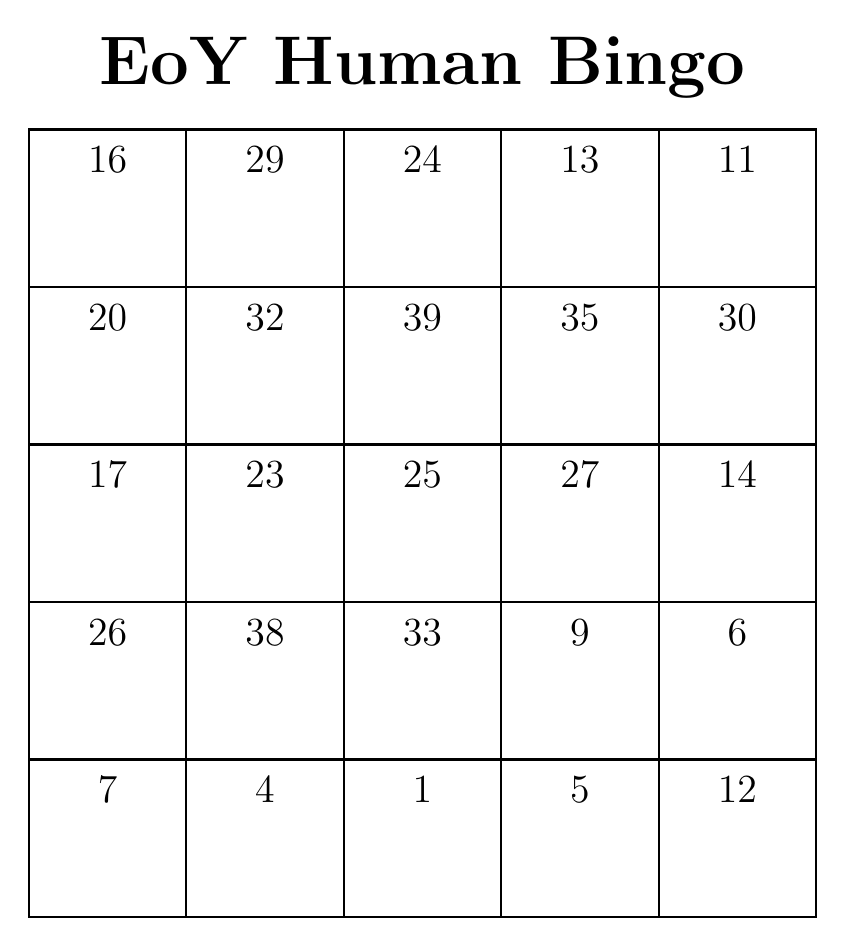
\begin{tikzpicture}
% Set the grid dimensions
\def\cellsize{2cm} % Each cell will be 2x2 cm

% Draw the grid and insert the numbers
\draw[thick] (0, 0) rectangle +(2, 2);
\node[anchor=north, font=\Large, align=center] at (1.0, 1.9) {16};
\draw[thick] (2, 0) rectangle +(2, 2);
\node[anchor=north, font=\Large, align=center] at (3.0, 1.9) {29};
\draw[thick] (4, 0) rectangle +(2, 2);
\node[anchor=north, font=\Large, align=center] at (5.0, 1.9) {24};
\draw[thick] (6, 0) rectangle +(2, 2);
\node[anchor=north, font=\Large, align=center] at (7.0, 1.9) {13};
\draw[thick] (8, 0) rectangle +(2, 2);
\node[anchor=north, font=\Large, align=center] at (9.0, 1.9) {11};
\draw[thick] (0, -2) rectangle +(2, 2);
\node[anchor=north, font=\Large, align=center] at (1.0, -0.1) {20};
\draw[thick] (2, -2) rectangle +(2, 2);
\node[anchor=north, font=\Large, align=center] at (3.0, -0.1) {32};
\draw[thick] (4, -2) rectangle +(2, 2);
\node[anchor=north, font=\Large, align=center] at (5.0, -0.1) {39};
\draw[thick] (6, -2) rectangle +(2, 2);
\node[anchor=north, font=\Large, align=center] at (7.0, -0.1) {35};
\draw[thick] (8, -2) rectangle +(2, 2);
\node[anchor=north, font=\Large, align=center] at (9.0, -0.1) {30};
\draw[thick] (0, -4) rectangle +(2, 2);
\node[anchor=north, font=\Large, align=center] at (1.0, -2.1) {17};
\draw[thick] (2, -4) rectangle +(2, 2);
\node[anchor=north, font=\Large, align=center] at (3.0, -2.1) {23};
\draw[thick] (4, -4) rectangle +(2, 2);
\node[anchor=north, font=\Large, align=center] at (5.0, -2.1) {25};
\draw[thick] (6, -4) rectangle +(2, 2);
\node[anchor=north, font=\Large, align=center] at (7.0, -2.1) {27};
\draw[thick] (8, -4) rectangle +(2, 2);
\node[anchor=north, font=\Large, align=center] at (9.0, -2.1) {14};
\draw[thick] (0, -6) rectangle +(2, 2);
\node[anchor=north, font=\Large, align=center] at (1.0, -4.1) {26};
\draw[thick] (2, -6) rectangle +(2, 2);
\node[anchor=north, font=\Large, align=center] at (3.0, -4.1) {38};
\draw[thick] (4, -6) rectangle +(2, 2);
\node[anchor=north, font=\Large, align=center] at (5.0, -4.1) {33};
\draw[thick] (6, -6) rectangle +(2, 2);
\node[anchor=north, font=\Large, align=center] at (7.0, -4.1) {9};
\draw[thick] (8, -6) rectangle +(2, 2);
\node[anchor=north, font=\Large, align=center] at (9.0, -4.1) {6};
\draw[thick] (0, -8) rectangle +(2, 2);
\node[anchor=north, font=\Large, align=center] at (1.0, -6.1) {7};
\draw[thick] (2, -8) rectangle +(2, 2);
\node[anchor=north, font=\Large, align=center] at (3.0, -6.1) {4};
\draw[thick] (4, -8) rectangle +(2, 2);
\node[anchor=north, font=\Large, align=center] at (5.0, -6.1) {1};
\draw[thick] (6, -8) rectangle +(2, 2);
\node[anchor=north, font=\Large, align=center] at (7.0, -6.1) {5};
\draw[thick] (8, -8) rectangle +(2, 2);
\node[anchor=north, font=\Large, align=center] at (9.0, -6.1) {12};
\node[anchor=north, font = \Huge] at (5.0, 3.3){\textbf{EoY Human Bingo}};
\end{tikzpicture}
\end{center}
\newpage\begin{center}
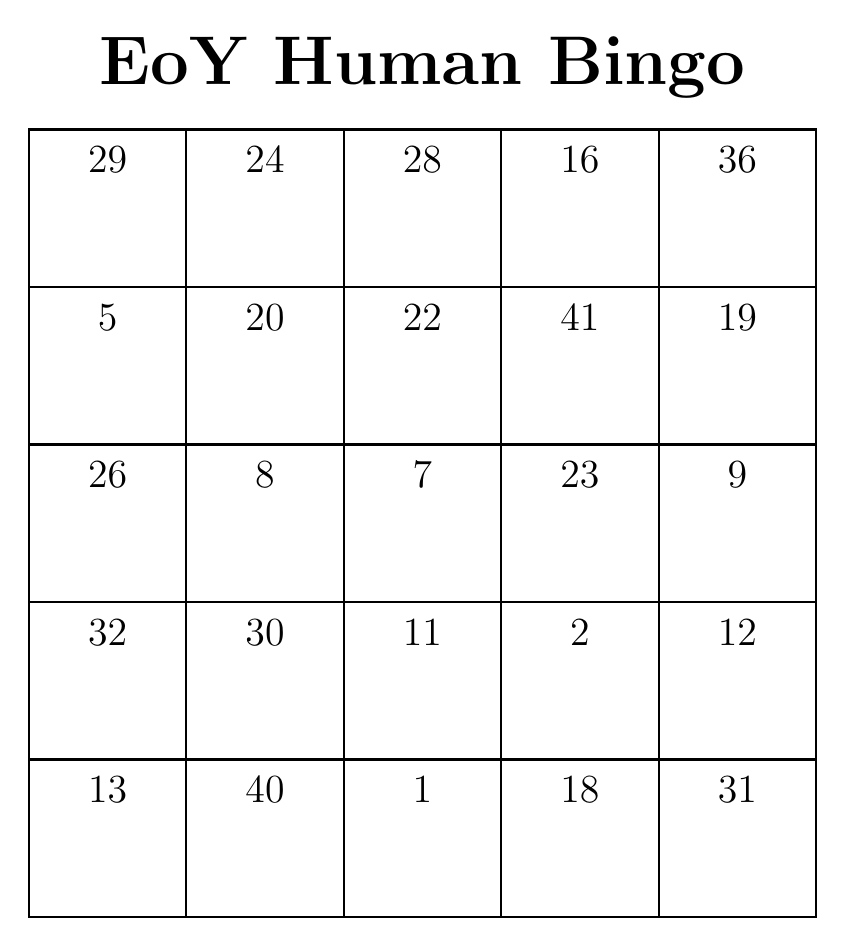
\begin{tikzpicture}
% Set the grid dimensions
\def\cellsize{2cm} % Each cell will be 2x2 cm

% Draw the grid and insert the numbers
\draw[thick] (0, 0) rectangle +(2, 2);
\node[anchor=north, font=\Large, align=center] at (1.0, 1.9) {29};
\draw[thick] (2, 0) rectangle +(2, 2);
\node[anchor=north, font=\Large, align=center] at (3.0, 1.9) {24};
\draw[thick] (4, 0) rectangle +(2, 2);
\node[anchor=north, font=\Large, align=center] at (5.0, 1.9) {28};
\draw[thick] (6, 0) rectangle +(2, 2);
\node[anchor=north, font=\Large, align=center] at (7.0, 1.9) {16};
\draw[thick] (8, 0) rectangle +(2, 2);
\node[anchor=north, font=\Large, align=center] at (9.0, 1.9) {36};
\draw[thick] (0, -2) rectangle +(2, 2);
\node[anchor=north, font=\Large, align=center] at (1.0, -0.1) {5};
\draw[thick] (2, -2) rectangle +(2, 2);
\node[anchor=north, font=\Large, align=center] at (3.0, -0.1) {20};
\draw[thick] (4, -2) rectangle +(2, 2);
\node[anchor=north, font=\Large, align=center] at (5.0, -0.1) {22};
\draw[thick] (6, -2) rectangle +(2, 2);
\node[anchor=north, font=\Large, align=center] at (7.0, -0.1) {41};
\draw[thick] (8, -2) rectangle +(2, 2);
\node[anchor=north, font=\Large, align=center] at (9.0, -0.1) {19};
\draw[thick] (0, -4) rectangle +(2, 2);
\node[anchor=north, font=\Large, align=center] at (1.0, -2.1) {26};
\draw[thick] (2, -4) rectangle +(2, 2);
\node[anchor=north, font=\Large, align=center] at (3.0, -2.1) {8};
\draw[thick] (4, -4) rectangle +(2, 2);
\node[anchor=north, font=\Large, align=center] at (5.0, -2.1) {7};
\draw[thick] (6, -4) rectangle +(2, 2);
\node[anchor=north, font=\Large, align=center] at (7.0, -2.1) {23};
\draw[thick] (8, -4) rectangle +(2, 2);
\node[anchor=north, font=\Large, align=center] at (9.0, -2.1) {9};
\draw[thick] (0, -6) rectangle +(2, 2);
\node[anchor=north, font=\Large, align=center] at (1.0, -4.1) {32};
\draw[thick] (2, -6) rectangle +(2, 2);
\node[anchor=north, font=\Large, align=center] at (3.0, -4.1) {30};
\draw[thick] (4, -6) rectangle +(2, 2);
\node[anchor=north, font=\Large, align=center] at (5.0, -4.1) {11};
\draw[thick] (6, -6) rectangle +(2, 2);
\node[anchor=north, font=\Large, align=center] at (7.0, -4.1) {2};
\draw[thick] (8, -6) rectangle +(2, 2);
\node[anchor=north, font=\Large, align=center] at (9.0, -4.1) {12};
\draw[thick] (0, -8) rectangle +(2, 2);
\node[anchor=north, font=\Large, align=center] at (1.0, -6.1) {13};
\draw[thick] (2, -8) rectangle +(2, 2);
\node[anchor=north, font=\Large, align=center] at (3.0, -6.1) {40};
\draw[thick] (4, -8) rectangle +(2, 2);
\node[anchor=north, font=\Large, align=center] at (5.0, -6.1) {1};
\draw[thick] (6, -8) rectangle +(2, 2);
\node[anchor=north, font=\Large, align=center] at (7.0, -6.1) {18};
\draw[thick] (8, -8) rectangle +(2, 2);
\node[anchor=north, font=\Large, align=center] at (9.0, -6.1) {31};
\node[anchor=north, font = \Huge] at (5.0, 3.3){\textbf{EoY Human Bingo}};
\end{tikzpicture}
\end{center}
\newpage\begin{center}
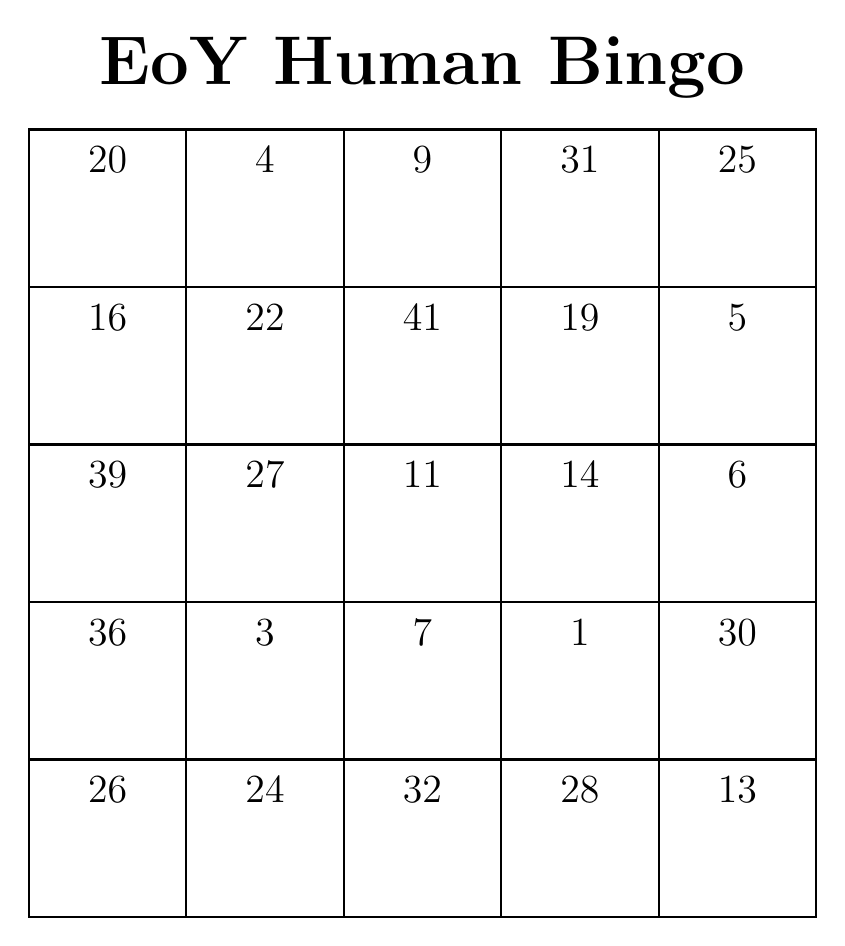
\begin{tikzpicture}
% Set the grid dimensions
\def\cellsize{2cm} % Each cell will be 2x2 cm

% Draw the grid and insert the numbers
\draw[thick] (0, 0) rectangle +(2, 2);
\node[anchor=north, font=\Large, align=center] at (1.0, 1.9) {20};
\draw[thick] (2, 0) rectangle +(2, 2);
\node[anchor=north, font=\Large, align=center] at (3.0, 1.9) {4};
\draw[thick] (4, 0) rectangle +(2, 2);
\node[anchor=north, font=\Large, align=center] at (5.0, 1.9) {9};
\draw[thick] (6, 0) rectangle +(2, 2);
\node[anchor=north, font=\Large, align=center] at (7.0, 1.9) {31};
\draw[thick] (8, 0) rectangle +(2, 2);
\node[anchor=north, font=\Large, align=center] at (9.0, 1.9) {25};
\draw[thick] (0, -2) rectangle +(2, 2);
\node[anchor=north, font=\Large, align=center] at (1.0, -0.1) {16};
\draw[thick] (2, -2) rectangle +(2, 2);
\node[anchor=north, font=\Large, align=center] at (3.0, -0.1) {22};
\draw[thick] (4, -2) rectangle +(2, 2);
\node[anchor=north, font=\Large, align=center] at (5.0, -0.1) {41};
\draw[thick] (6, -2) rectangle +(2, 2);
\node[anchor=north, font=\Large, align=center] at (7.0, -0.1) {19};
\draw[thick] (8, -2) rectangle +(2, 2);
\node[anchor=north, font=\Large, align=center] at (9.0, -0.1) {5};
\draw[thick] (0, -4) rectangle +(2, 2);
\node[anchor=north, font=\Large, align=center] at (1.0, -2.1) {39};
\draw[thick] (2, -4) rectangle +(2, 2);
\node[anchor=north, font=\Large, align=center] at (3.0, -2.1) {27};
\draw[thick] (4, -4) rectangle +(2, 2);
\node[anchor=north, font=\Large, align=center] at (5.0, -2.1) {11};
\draw[thick] (6, -4) rectangle +(2, 2);
\node[anchor=north, font=\Large, align=center] at (7.0, -2.1) {14};
\draw[thick] (8, -4) rectangle +(2, 2);
\node[anchor=north, font=\Large, align=center] at (9.0, -2.1) {6};
\draw[thick] (0, -6) rectangle +(2, 2);
\node[anchor=north, font=\Large, align=center] at (1.0, -4.1) {36};
\draw[thick] (2, -6) rectangle +(2, 2);
\node[anchor=north, font=\Large, align=center] at (3.0, -4.1) {3};
\draw[thick] (4, -6) rectangle +(2, 2);
\node[anchor=north, font=\Large, align=center] at (5.0, -4.1) {7};
\draw[thick] (6, -6) rectangle +(2, 2);
\node[anchor=north, font=\Large, align=center] at (7.0, -4.1) {1};
\draw[thick] (8, -6) rectangle +(2, 2);
\node[anchor=north, font=\Large, align=center] at (9.0, -4.1) {30};
\draw[thick] (0, -8) rectangle +(2, 2);
\node[anchor=north, font=\Large, align=center] at (1.0, -6.1) {26};
\draw[thick] (2, -8) rectangle +(2, 2);
\node[anchor=north, font=\Large, align=center] at (3.0, -6.1) {24};
\draw[thick] (4, -8) rectangle +(2, 2);
\node[anchor=north, font=\Large, align=center] at (5.0, -6.1) {32};
\draw[thick] (6, -8) rectangle +(2, 2);
\node[anchor=north, font=\Large, align=center] at (7.0, -6.1) {28};
\draw[thick] (8, -8) rectangle +(2, 2);
\node[anchor=north, font=\Large, align=center] at (9.0, -6.1) {13};
\node[anchor=north, font = \Huge] at (5.0, 3.3){\textbf{EoY Human Bingo}};
\end{tikzpicture}
\end{center}
\newpage\begin{center}
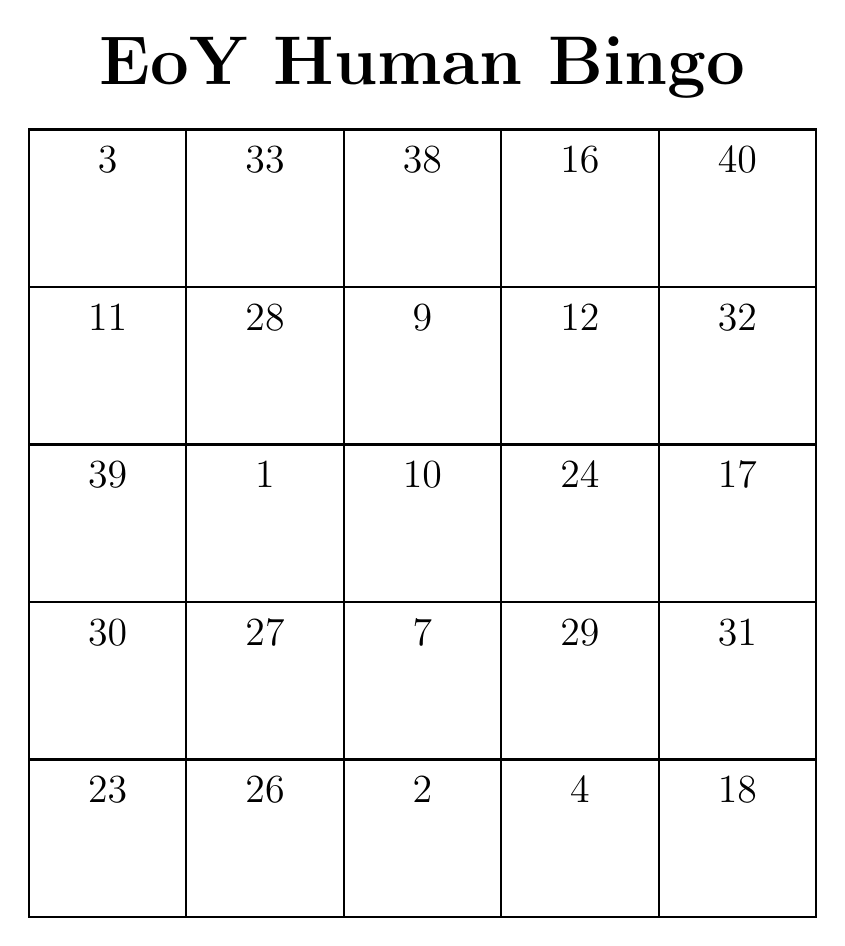
\begin{tikzpicture}
% Set the grid dimensions
\def\cellsize{2cm} % Each cell will be 2x2 cm

% Draw the grid and insert the numbers
\draw[thick] (0, 0) rectangle +(2, 2);
\node[anchor=north, font=\Large, align=center] at (1.0, 1.9) {3};
\draw[thick] (2, 0) rectangle +(2, 2);
\node[anchor=north, font=\Large, align=center] at (3.0, 1.9) {33};
\draw[thick] (4, 0) rectangle +(2, 2);
\node[anchor=north, font=\Large, align=center] at (5.0, 1.9) {38};
\draw[thick] (6, 0) rectangle +(2, 2);
\node[anchor=north, font=\Large, align=center] at (7.0, 1.9) {16};
\draw[thick] (8, 0) rectangle +(2, 2);
\node[anchor=north, font=\Large, align=center] at (9.0, 1.9) {40};
\draw[thick] (0, -2) rectangle +(2, 2);
\node[anchor=north, font=\Large, align=center] at (1.0, -0.1) {11};
\draw[thick] (2, -2) rectangle +(2, 2);
\node[anchor=north, font=\Large, align=center] at (3.0, -0.1) {28};
\draw[thick] (4, -2) rectangle +(2, 2);
\node[anchor=north, font=\Large, align=center] at (5.0, -0.1) {9};
\draw[thick] (6, -2) rectangle +(2, 2);
\node[anchor=north, font=\Large, align=center] at (7.0, -0.1) {12};
\draw[thick] (8, -2) rectangle +(2, 2);
\node[anchor=north, font=\Large, align=center] at (9.0, -0.1) {32};
\draw[thick] (0, -4) rectangle +(2, 2);
\node[anchor=north, font=\Large, align=center] at (1.0, -2.1) {39};
\draw[thick] (2, -4) rectangle +(2, 2);
\node[anchor=north, font=\Large, align=center] at (3.0, -2.1) {1};
\draw[thick] (4, -4) rectangle +(2, 2);
\node[anchor=north, font=\Large, align=center] at (5.0, -2.1) {10};
\draw[thick] (6, -4) rectangle +(2, 2);
\node[anchor=north, font=\Large, align=center] at (7.0, -2.1) {24};
\draw[thick] (8, -4) rectangle +(2, 2);
\node[anchor=north, font=\Large, align=center] at (9.0, -2.1) {17};
\draw[thick] (0, -6) rectangle +(2, 2);
\node[anchor=north, font=\Large, align=center] at (1.0, -4.1) {30};
\draw[thick] (2, -6) rectangle +(2, 2);
\node[anchor=north, font=\Large, align=center] at (3.0, -4.1) {27};
\draw[thick] (4, -6) rectangle +(2, 2);
\node[anchor=north, font=\Large, align=center] at (5.0, -4.1) {7};
\draw[thick] (6, -6) rectangle +(2, 2);
\node[anchor=north, font=\Large, align=center] at (7.0, -4.1) {29};
\draw[thick] (8, -6) rectangle +(2, 2);
\node[anchor=north, font=\Large, align=center] at (9.0, -4.1) {31};
\draw[thick] (0, -8) rectangle +(2, 2);
\node[anchor=north, font=\Large, align=center] at (1.0, -6.1) {23};
\draw[thick] (2, -8) rectangle +(2, 2);
\node[anchor=north, font=\Large, align=center] at (3.0, -6.1) {26};
\draw[thick] (4, -8) rectangle +(2, 2);
\node[anchor=north, font=\Large, align=center] at (5.0, -6.1) {2};
\draw[thick] (6, -8) rectangle +(2, 2);
\node[anchor=north, font=\Large, align=center] at (7.0, -6.1) {4};
\draw[thick] (8, -8) rectangle +(2, 2);
\node[anchor=north, font=\Large, align=center] at (9.0, -6.1) {18};
\node[anchor=north, font = \Huge] at (5.0, 3.3){\textbf{EoY Human Bingo}};
\end{tikzpicture}
\end{center}
\newpage\begin{center}
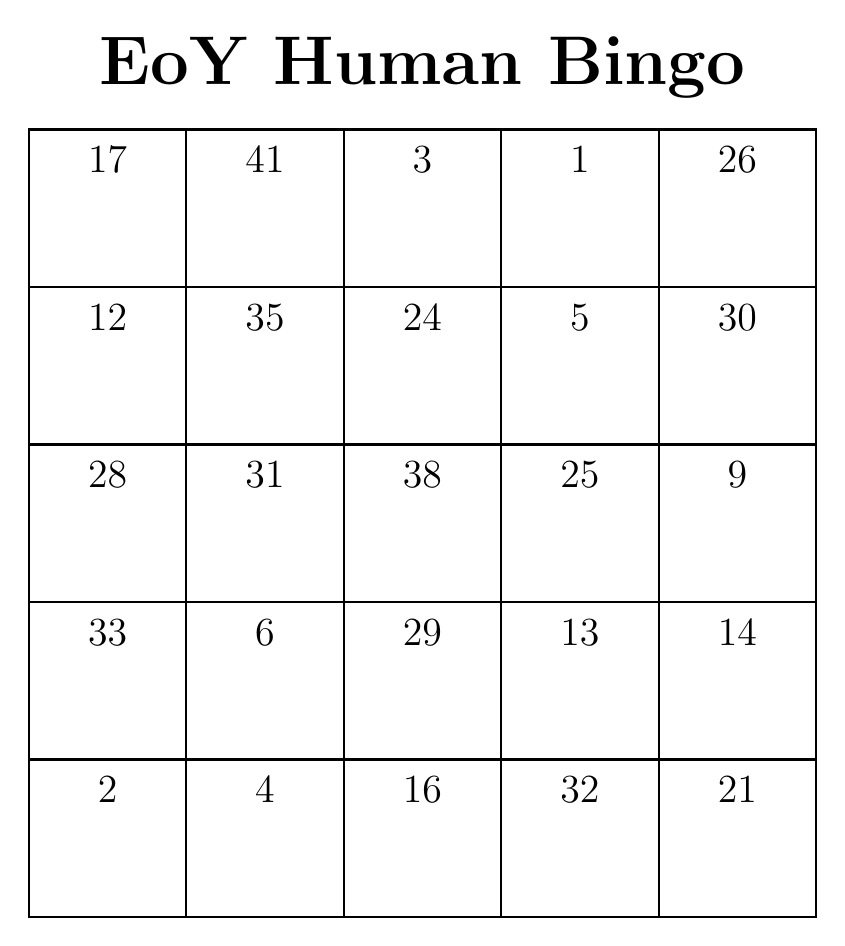
\begin{tikzpicture}
% Set the grid dimensions
\def\cellsize{2cm} % Each cell will be 2x2 cm

% Draw the grid and insert the numbers
\draw[thick] (0, 0) rectangle +(2, 2);
\node[anchor=north, font=\Large, align=center] at (1.0, 1.9) {17};
\draw[thick] (2, 0) rectangle +(2, 2);
\node[anchor=north, font=\Large, align=center] at (3.0, 1.9) {41};
\draw[thick] (4, 0) rectangle +(2, 2);
\node[anchor=north, font=\Large, align=center] at (5.0, 1.9) {3};
\draw[thick] (6, 0) rectangle +(2, 2);
\node[anchor=north, font=\Large, align=center] at (7.0, 1.9) {1};
\draw[thick] (8, 0) rectangle +(2, 2);
\node[anchor=north, font=\Large, align=center] at (9.0, 1.9) {26};
\draw[thick] (0, -2) rectangle +(2, 2);
\node[anchor=north, font=\Large, align=center] at (1.0, -0.1) {12};
\draw[thick] (2, -2) rectangle +(2, 2);
\node[anchor=north, font=\Large, align=center] at (3.0, -0.1) {35};
\draw[thick] (4, -2) rectangle +(2, 2);
\node[anchor=north, font=\Large, align=center] at (5.0, -0.1) {24};
\draw[thick] (6, -2) rectangle +(2, 2);
\node[anchor=north, font=\Large, align=center] at (7.0, -0.1) {5};
\draw[thick] (8, -2) rectangle +(2, 2);
\node[anchor=north, font=\Large, align=center] at (9.0, -0.1) {30};
\draw[thick] (0, -4) rectangle +(2, 2);
\node[anchor=north, font=\Large, align=center] at (1.0, -2.1) {28};
\draw[thick] (2, -4) rectangle +(2, 2);
\node[anchor=north, font=\Large, align=center] at (3.0, -2.1) {31};
\draw[thick] (4, -4) rectangle +(2, 2);
\node[anchor=north, font=\Large, align=center] at (5.0, -2.1) {38};
\draw[thick] (6, -4) rectangle +(2, 2);
\node[anchor=north, font=\Large, align=center] at (7.0, -2.1) {25};
\draw[thick] (8, -4) rectangle +(2, 2);
\node[anchor=north, font=\Large, align=center] at (9.0, -2.1) {9};
\draw[thick] (0, -6) rectangle +(2, 2);
\node[anchor=north, font=\Large, align=center] at (1.0, -4.1) {33};
\draw[thick] (2, -6) rectangle +(2, 2);
\node[anchor=north, font=\Large, align=center] at (3.0, -4.1) {6};
\draw[thick] (4, -6) rectangle +(2, 2);
\node[anchor=north, font=\Large, align=center] at (5.0, -4.1) {29};
\draw[thick] (6, -6) rectangle +(2, 2);
\node[anchor=north, font=\Large, align=center] at (7.0, -4.1) {13};
\draw[thick] (8, -6) rectangle +(2, 2);
\node[anchor=north, font=\Large, align=center] at (9.0, -4.1) {14};
\draw[thick] (0, -8) rectangle +(2, 2);
\node[anchor=north, font=\Large, align=center] at (1.0, -6.1) {2};
\draw[thick] (2, -8) rectangle +(2, 2);
\node[anchor=north, font=\Large, align=center] at (3.0, -6.1) {4};
\draw[thick] (4, -8) rectangle +(2, 2);
\node[anchor=north, font=\Large, align=center] at (5.0, -6.1) {16};
\draw[thick] (6, -8) rectangle +(2, 2);
\node[anchor=north, font=\Large, align=center] at (7.0, -6.1) {32};
\draw[thick] (8, -8) rectangle +(2, 2);
\node[anchor=north, font=\Large, align=center] at (9.0, -6.1) {21};
\node[anchor=north, font = \Huge] at (5.0, 3.3){\textbf{EoY Human Bingo}};
\end{tikzpicture}
\end{center}
\newpage\begin{center}
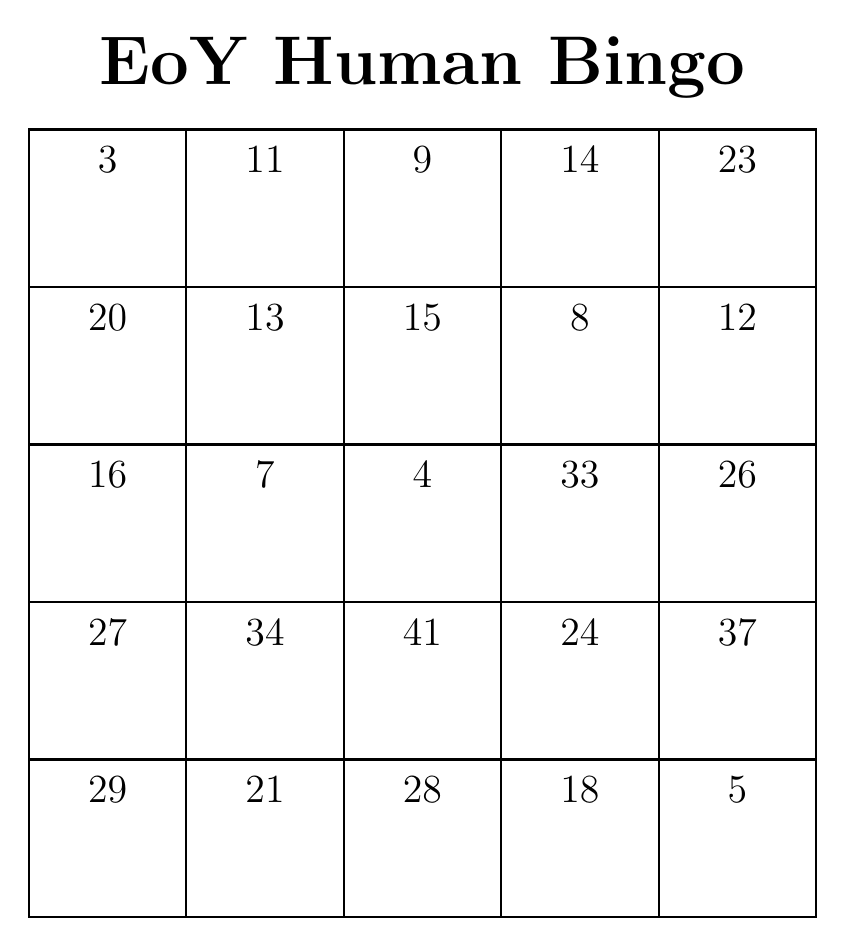
\begin{tikzpicture}
% Set the grid dimensions
\def\cellsize{2cm} % Each cell will be 2x2 cm

% Draw the grid and insert the numbers
\draw[thick] (0, 0) rectangle +(2, 2);
\node[anchor=north, font=\Large, align=center] at (1.0, 1.9) {3};
\draw[thick] (2, 0) rectangle +(2, 2);
\node[anchor=north, font=\Large, align=center] at (3.0, 1.9) {11};
\draw[thick] (4, 0) rectangle +(2, 2);
\node[anchor=north, font=\Large, align=center] at (5.0, 1.9) {9};
\draw[thick] (6, 0) rectangle +(2, 2);
\node[anchor=north, font=\Large, align=center] at (7.0, 1.9) {14};
\draw[thick] (8, 0) rectangle +(2, 2);
\node[anchor=north, font=\Large, align=center] at (9.0, 1.9) {23};
\draw[thick] (0, -2) rectangle +(2, 2);
\node[anchor=north, font=\Large, align=center] at (1.0, -0.1) {20};
\draw[thick] (2, -2) rectangle +(2, 2);
\node[anchor=north, font=\Large, align=center] at (3.0, -0.1) {13};
\draw[thick] (4, -2) rectangle +(2, 2);
\node[anchor=north, font=\Large, align=center] at (5.0, -0.1) {15};
\draw[thick] (6, -2) rectangle +(2, 2);
\node[anchor=north, font=\Large, align=center] at (7.0, -0.1) {8};
\draw[thick] (8, -2) rectangle +(2, 2);
\node[anchor=north, font=\Large, align=center] at (9.0, -0.1) {12};
\draw[thick] (0, -4) rectangle +(2, 2);
\node[anchor=north, font=\Large, align=center] at (1.0, -2.1) {16};
\draw[thick] (2, -4) rectangle +(2, 2);
\node[anchor=north, font=\Large, align=center] at (3.0, -2.1) {7};
\draw[thick] (4, -4) rectangle +(2, 2);
\node[anchor=north, font=\Large, align=center] at (5.0, -2.1) {4};
\draw[thick] (6, -4) rectangle +(2, 2);
\node[anchor=north, font=\Large, align=center] at (7.0, -2.1) {33};
\draw[thick] (8, -4) rectangle +(2, 2);
\node[anchor=north, font=\Large, align=center] at (9.0, -2.1) {26};
\draw[thick] (0, -6) rectangle +(2, 2);
\node[anchor=north, font=\Large, align=center] at (1.0, -4.1) {27};
\draw[thick] (2, -6) rectangle +(2, 2);
\node[anchor=north, font=\Large, align=center] at (3.0, -4.1) {34};
\draw[thick] (4, -6) rectangle +(2, 2);
\node[anchor=north, font=\Large, align=center] at (5.0, -4.1) {41};
\draw[thick] (6, -6) rectangle +(2, 2);
\node[anchor=north, font=\Large, align=center] at (7.0, -4.1) {24};
\draw[thick] (8, -6) rectangle +(2, 2);
\node[anchor=north, font=\Large, align=center] at (9.0, -4.1) {37};
\draw[thick] (0, -8) rectangle +(2, 2);
\node[anchor=north, font=\Large, align=center] at (1.0, -6.1) {29};
\draw[thick] (2, -8) rectangle +(2, 2);
\node[anchor=north, font=\Large, align=center] at (3.0, -6.1) {21};
\draw[thick] (4, -8) rectangle +(2, 2);
\node[anchor=north, font=\Large, align=center] at (5.0, -6.1) {28};
\draw[thick] (6, -8) rectangle +(2, 2);
\node[anchor=north, font=\Large, align=center] at (7.0, -6.1) {18};
\draw[thick] (8, -8) rectangle +(2, 2);
\node[anchor=north, font=\Large, align=center] at (9.0, -6.1) {5};
\node[anchor=north, font = \Huge] at (5.0, 3.3){\textbf{EoY Human Bingo}};
\end{tikzpicture}
\end{center}
\newpage\begin{center}
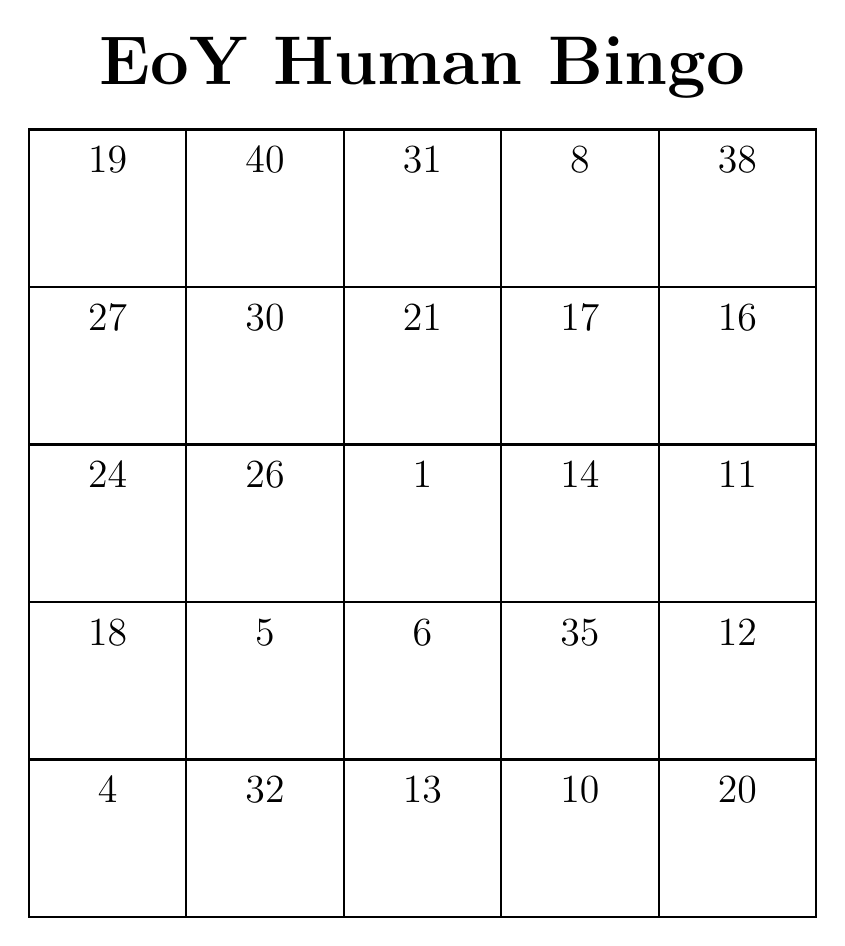
\begin{tikzpicture}
% Set the grid dimensions
\def\cellsize{2cm} % Each cell will be 2x2 cm

% Draw the grid and insert the numbers
\draw[thick] (0, 0) rectangle +(2, 2);
\node[anchor=north, font=\Large, align=center] at (1.0, 1.9) {19};
\draw[thick] (2, 0) rectangle +(2, 2);
\node[anchor=north, font=\Large, align=center] at (3.0, 1.9) {40};
\draw[thick] (4, 0) rectangle +(2, 2);
\node[anchor=north, font=\Large, align=center] at (5.0, 1.9) {31};
\draw[thick] (6, 0) rectangle +(2, 2);
\node[anchor=north, font=\Large, align=center] at (7.0, 1.9) {8};
\draw[thick] (8, 0) rectangle +(2, 2);
\node[anchor=north, font=\Large, align=center] at (9.0, 1.9) {38};
\draw[thick] (0, -2) rectangle +(2, 2);
\node[anchor=north, font=\Large, align=center] at (1.0, -0.1) {27};
\draw[thick] (2, -2) rectangle +(2, 2);
\node[anchor=north, font=\Large, align=center] at (3.0, -0.1) {30};
\draw[thick] (4, -2) rectangle +(2, 2);
\node[anchor=north, font=\Large, align=center] at (5.0, -0.1) {21};
\draw[thick] (6, -2) rectangle +(2, 2);
\node[anchor=north, font=\Large, align=center] at (7.0, -0.1) {17};
\draw[thick] (8, -2) rectangle +(2, 2);
\node[anchor=north, font=\Large, align=center] at (9.0, -0.1) {16};
\draw[thick] (0, -4) rectangle +(2, 2);
\node[anchor=north, font=\Large, align=center] at (1.0, -2.1) {24};
\draw[thick] (2, -4) rectangle +(2, 2);
\node[anchor=north, font=\Large, align=center] at (3.0, -2.1) {26};
\draw[thick] (4, -4) rectangle +(2, 2);
\node[anchor=north, font=\Large, align=center] at (5.0, -2.1) {1};
\draw[thick] (6, -4) rectangle +(2, 2);
\node[anchor=north, font=\Large, align=center] at (7.0, -2.1) {14};
\draw[thick] (8, -4) rectangle +(2, 2);
\node[anchor=north, font=\Large, align=center] at (9.0, -2.1) {11};
\draw[thick] (0, -6) rectangle +(2, 2);
\node[anchor=north, font=\Large, align=center] at (1.0, -4.1) {18};
\draw[thick] (2, -6) rectangle +(2, 2);
\node[anchor=north, font=\Large, align=center] at (3.0, -4.1) {5};
\draw[thick] (4, -6) rectangle +(2, 2);
\node[anchor=north, font=\Large, align=center] at (5.0, -4.1) {6};
\draw[thick] (6, -6) rectangle +(2, 2);
\node[anchor=north, font=\Large, align=center] at (7.0, -4.1) {35};
\draw[thick] (8, -6) rectangle +(2, 2);
\node[anchor=north, font=\Large, align=center] at (9.0, -4.1) {12};
\draw[thick] (0, -8) rectangle +(2, 2);
\node[anchor=north, font=\Large, align=center] at (1.0, -6.1) {4};
\draw[thick] (2, -8) rectangle +(2, 2);
\node[anchor=north, font=\Large, align=center] at (3.0, -6.1) {32};
\draw[thick] (4, -8) rectangle +(2, 2);
\node[anchor=north, font=\Large, align=center] at (5.0, -6.1) {13};
\draw[thick] (6, -8) rectangle +(2, 2);
\node[anchor=north, font=\Large, align=center] at (7.0, -6.1) {10};
\draw[thick] (8, -8) rectangle +(2, 2);
\node[anchor=north, font=\Large, align=center] at (9.0, -6.1) {20};
\node[anchor=north, font = \Huge] at (5.0, 3.3){\textbf{EoY Human Bingo}};
\end{tikzpicture}
\end{center}
\newpage\begin{center}
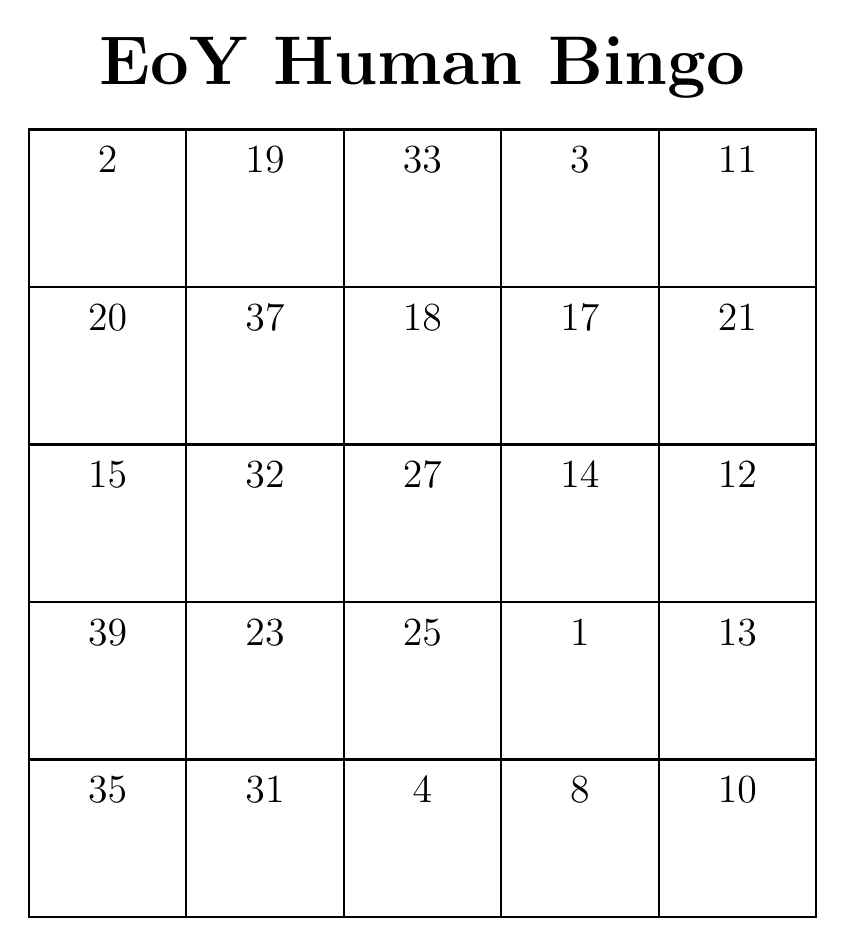
\begin{tikzpicture}
% Set the grid dimensions
\def\cellsize{2cm} % Each cell will be 2x2 cm

% Draw the grid and insert the numbers
\draw[thick] (0, 0) rectangle +(2, 2);
\node[anchor=north, font=\Large, align=center] at (1.0, 1.9) {2};
\draw[thick] (2, 0) rectangle +(2, 2);
\node[anchor=north, font=\Large, align=center] at (3.0, 1.9) {19};
\draw[thick] (4, 0) rectangle +(2, 2);
\node[anchor=north, font=\Large, align=center] at (5.0, 1.9) {33};
\draw[thick] (6, 0) rectangle +(2, 2);
\node[anchor=north, font=\Large, align=center] at (7.0, 1.9) {3};
\draw[thick] (8, 0) rectangle +(2, 2);
\node[anchor=north, font=\Large, align=center] at (9.0, 1.9) {11};
\draw[thick] (0, -2) rectangle +(2, 2);
\node[anchor=north, font=\Large, align=center] at (1.0, -0.1) {20};
\draw[thick] (2, -2) rectangle +(2, 2);
\node[anchor=north, font=\Large, align=center] at (3.0, -0.1) {37};
\draw[thick] (4, -2) rectangle +(2, 2);
\node[anchor=north, font=\Large, align=center] at (5.0, -0.1) {18};
\draw[thick] (6, -2) rectangle +(2, 2);
\node[anchor=north, font=\Large, align=center] at (7.0, -0.1) {17};
\draw[thick] (8, -2) rectangle +(2, 2);
\node[anchor=north, font=\Large, align=center] at (9.0, -0.1) {21};
\draw[thick] (0, -4) rectangle +(2, 2);
\node[anchor=north, font=\Large, align=center] at (1.0, -2.1) {15};
\draw[thick] (2, -4) rectangle +(2, 2);
\node[anchor=north, font=\Large, align=center] at (3.0, -2.1) {32};
\draw[thick] (4, -4) rectangle +(2, 2);
\node[anchor=north, font=\Large, align=center] at (5.0, -2.1) {27};
\draw[thick] (6, -4) rectangle +(2, 2);
\node[anchor=north, font=\Large, align=center] at (7.0, -2.1) {14};
\draw[thick] (8, -4) rectangle +(2, 2);
\node[anchor=north, font=\Large, align=center] at (9.0, -2.1) {12};
\draw[thick] (0, -6) rectangle +(2, 2);
\node[anchor=north, font=\Large, align=center] at (1.0, -4.1) {39};
\draw[thick] (2, -6) rectangle +(2, 2);
\node[anchor=north, font=\Large, align=center] at (3.0, -4.1) {23};
\draw[thick] (4, -6) rectangle +(2, 2);
\node[anchor=north, font=\Large, align=center] at (5.0, -4.1) {25};
\draw[thick] (6, -6) rectangle +(2, 2);
\node[anchor=north, font=\Large, align=center] at (7.0, -4.1) {1};
\draw[thick] (8, -6) rectangle +(2, 2);
\node[anchor=north, font=\Large, align=center] at (9.0, -4.1) {13};
\draw[thick] (0, -8) rectangle +(2, 2);
\node[anchor=north, font=\Large, align=center] at (1.0, -6.1) {35};
\draw[thick] (2, -8) rectangle +(2, 2);
\node[anchor=north, font=\Large, align=center] at (3.0, -6.1) {31};
\draw[thick] (4, -8) rectangle +(2, 2);
\node[anchor=north, font=\Large, align=center] at (5.0, -6.1) {4};
\draw[thick] (6, -8) rectangle +(2, 2);
\node[anchor=north, font=\Large, align=center] at (7.0, -6.1) {8};
\draw[thick] (8, -8) rectangle +(2, 2);
\node[anchor=north, font=\Large, align=center] at (9.0, -6.1) {10};
\node[anchor=north, font = \Huge] at (5.0, 3.3){\textbf{EoY Human Bingo}};
\end{tikzpicture}
\end{center}
\newpage\begin{center}
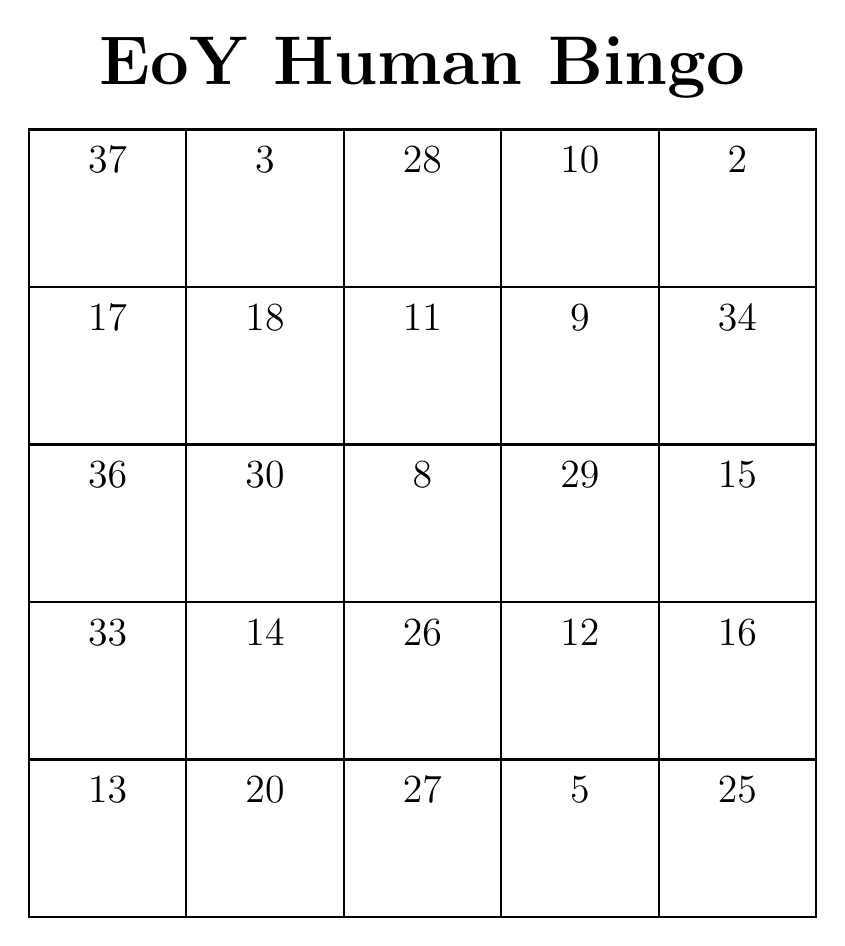
\begin{tikzpicture}
% Set the grid dimensions
\def\cellsize{2cm} % Each cell will be 2x2 cm

% Draw the grid and insert the numbers
\draw[thick] (0, 0) rectangle +(2, 2);
\node[anchor=north, font=\Large, align=center] at (1.0, 1.9) {37};
\draw[thick] (2, 0) rectangle +(2, 2);
\node[anchor=north, font=\Large, align=center] at (3.0, 1.9) {3};
\draw[thick] (4, 0) rectangle +(2, 2);
\node[anchor=north, font=\Large, align=center] at (5.0, 1.9) {28};
\draw[thick] (6, 0) rectangle +(2, 2);
\node[anchor=north, font=\Large, align=center] at (7.0, 1.9) {10};
\draw[thick] (8, 0) rectangle +(2, 2);
\node[anchor=north, font=\Large, align=center] at (9.0, 1.9) {2};
\draw[thick] (0, -2) rectangle +(2, 2);
\node[anchor=north, font=\Large, align=center] at (1.0, -0.1) {17};
\draw[thick] (2, -2) rectangle +(2, 2);
\node[anchor=north, font=\Large, align=center] at (3.0, -0.1) {18};
\draw[thick] (4, -2) rectangle +(2, 2);
\node[anchor=north, font=\Large, align=center] at (5.0, -0.1) {11};
\draw[thick] (6, -2) rectangle +(2, 2);
\node[anchor=north, font=\Large, align=center] at (7.0, -0.1) {9};
\draw[thick] (8, -2) rectangle +(2, 2);
\node[anchor=north, font=\Large, align=center] at (9.0, -0.1) {34};
\draw[thick] (0, -4) rectangle +(2, 2);
\node[anchor=north, font=\Large, align=center] at (1.0, -2.1) {36};
\draw[thick] (2, -4) rectangle +(2, 2);
\node[anchor=north, font=\Large, align=center] at (3.0, -2.1) {30};
\draw[thick] (4, -4) rectangle +(2, 2);
\node[anchor=north, font=\Large, align=center] at (5.0, -2.1) {8};
\draw[thick] (6, -4) rectangle +(2, 2);
\node[anchor=north, font=\Large, align=center] at (7.0, -2.1) {29};
\draw[thick] (8, -4) rectangle +(2, 2);
\node[anchor=north, font=\Large, align=center] at (9.0, -2.1) {15};
\draw[thick] (0, -6) rectangle +(2, 2);
\node[anchor=north, font=\Large, align=center] at (1.0, -4.1) {33};
\draw[thick] (2, -6) rectangle +(2, 2);
\node[anchor=north, font=\Large, align=center] at (3.0, -4.1) {14};
\draw[thick] (4, -6) rectangle +(2, 2);
\node[anchor=north, font=\Large, align=center] at (5.0, -4.1) {26};
\draw[thick] (6, -6) rectangle +(2, 2);
\node[anchor=north, font=\Large, align=center] at (7.0, -4.1) {12};
\draw[thick] (8, -6) rectangle +(2, 2);
\node[anchor=north, font=\Large, align=center] at (9.0, -4.1) {16};
\draw[thick] (0, -8) rectangle +(2, 2);
\node[anchor=north, font=\Large, align=center] at (1.0, -6.1) {13};
\draw[thick] (2, -8) rectangle +(2, 2);
\node[anchor=north, font=\Large, align=center] at (3.0, -6.1) {20};
\draw[thick] (4, -8) rectangle +(2, 2);
\node[anchor=north, font=\Large, align=center] at (5.0, -6.1) {27};
\draw[thick] (6, -8) rectangle +(2, 2);
\node[anchor=north, font=\Large, align=center] at (7.0, -6.1) {5};
\draw[thick] (8, -8) rectangle +(2, 2);
\node[anchor=north, font=\Large, align=center] at (9.0, -6.1) {25};
\node[anchor=north, font = \Huge] at (5.0, 3.3){\textbf{EoY Human Bingo}};
\end{tikzpicture}
\end{center}
\newpage\begin{center}
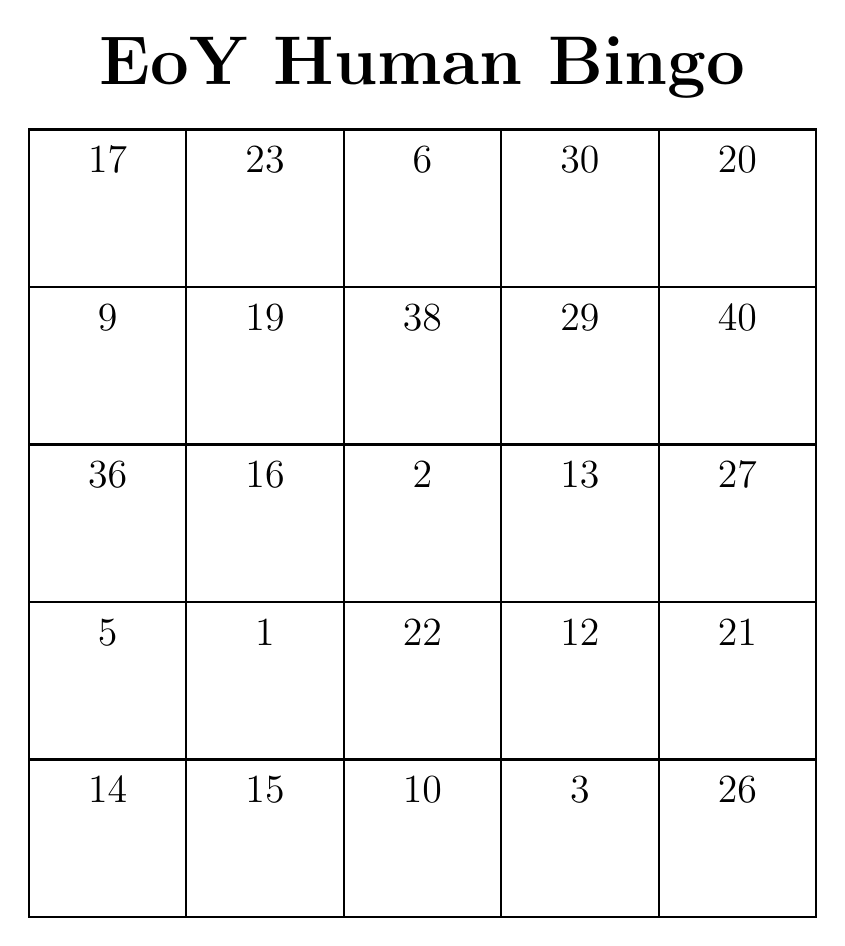
\begin{tikzpicture}
% Set the grid dimensions
\def\cellsize{2cm} % Each cell will be 2x2 cm

% Draw the grid and insert the numbers
\draw[thick] (0, 0) rectangle +(2, 2);
\node[anchor=north, font=\Large, align=center] at (1.0, 1.9) {17};
\draw[thick] (2, 0) rectangle +(2, 2);
\node[anchor=north, font=\Large, align=center] at (3.0, 1.9) {23};
\draw[thick] (4, 0) rectangle +(2, 2);
\node[anchor=north, font=\Large, align=center] at (5.0, 1.9) {6};
\draw[thick] (6, 0) rectangle +(2, 2);
\node[anchor=north, font=\Large, align=center] at (7.0, 1.9) {30};
\draw[thick] (8, 0) rectangle +(2, 2);
\node[anchor=north, font=\Large, align=center] at (9.0, 1.9) {20};
\draw[thick] (0, -2) rectangle +(2, 2);
\node[anchor=north, font=\Large, align=center] at (1.0, -0.1) {9};
\draw[thick] (2, -2) rectangle +(2, 2);
\node[anchor=north, font=\Large, align=center] at (3.0, -0.1) {19};
\draw[thick] (4, -2) rectangle +(2, 2);
\node[anchor=north, font=\Large, align=center] at (5.0, -0.1) {38};
\draw[thick] (6, -2) rectangle +(2, 2);
\node[anchor=north, font=\Large, align=center] at (7.0, -0.1) {29};
\draw[thick] (8, -2) rectangle +(2, 2);
\node[anchor=north, font=\Large, align=center] at (9.0, -0.1) {40};
\draw[thick] (0, -4) rectangle +(2, 2);
\node[anchor=north, font=\Large, align=center] at (1.0, -2.1) {36};
\draw[thick] (2, -4) rectangle +(2, 2);
\node[anchor=north, font=\Large, align=center] at (3.0, -2.1) {16};
\draw[thick] (4, -4) rectangle +(2, 2);
\node[anchor=north, font=\Large, align=center] at (5.0, -2.1) {2};
\draw[thick] (6, -4) rectangle +(2, 2);
\node[anchor=north, font=\Large, align=center] at (7.0, -2.1) {13};
\draw[thick] (8, -4) rectangle +(2, 2);
\node[anchor=north, font=\Large, align=center] at (9.0, -2.1) {27};
\draw[thick] (0, -6) rectangle +(2, 2);
\node[anchor=north, font=\Large, align=center] at (1.0, -4.1) {5};
\draw[thick] (2, -6) rectangle +(2, 2);
\node[anchor=north, font=\Large, align=center] at (3.0, -4.1) {1};
\draw[thick] (4, -6) rectangle +(2, 2);
\node[anchor=north, font=\Large, align=center] at (5.0, -4.1) {22};
\draw[thick] (6, -6) rectangle +(2, 2);
\node[anchor=north, font=\Large, align=center] at (7.0, -4.1) {12};
\draw[thick] (8, -6) rectangle +(2, 2);
\node[anchor=north, font=\Large, align=center] at (9.0, -4.1) {21};
\draw[thick] (0, -8) rectangle +(2, 2);
\node[anchor=north, font=\Large, align=center] at (1.0, -6.1) {14};
\draw[thick] (2, -8) rectangle +(2, 2);
\node[anchor=north, font=\Large, align=center] at (3.0, -6.1) {15};
\draw[thick] (4, -8) rectangle +(2, 2);
\node[anchor=north, font=\Large, align=center] at (5.0, -6.1) {10};
\draw[thick] (6, -8) rectangle +(2, 2);
\node[anchor=north, font=\Large, align=center] at (7.0, -6.1) {3};
\draw[thick] (8, -8) rectangle +(2, 2);
\node[anchor=north, font=\Large, align=center] at (9.0, -6.1) {26};
\node[anchor=north, font = \Huge] at (5.0, 3.3){\textbf{EoY Human Bingo}};
\end{tikzpicture}
\end{center}
\newpage\begin{center}
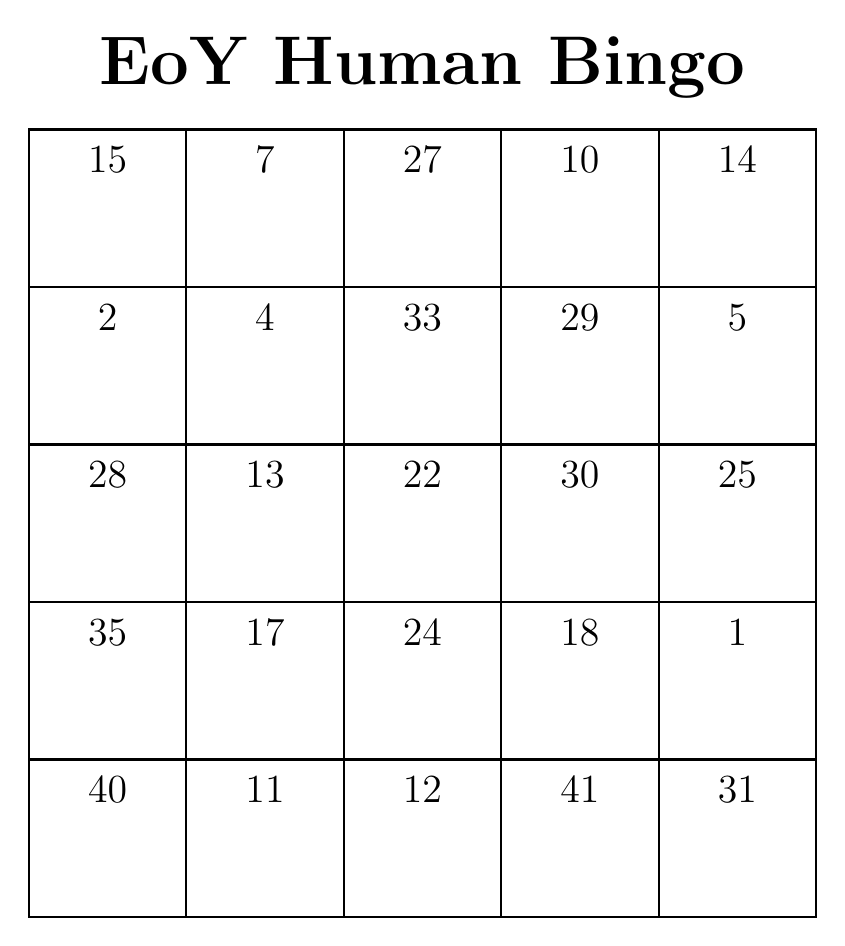
\begin{tikzpicture}
% Set the grid dimensions
\def\cellsize{2cm} % Each cell will be 2x2 cm

% Draw the grid and insert the numbers
\draw[thick] (0, 0) rectangle +(2, 2);
\node[anchor=north, font=\Large, align=center] at (1.0, 1.9) {15};
\draw[thick] (2, 0) rectangle +(2, 2);
\node[anchor=north, font=\Large, align=center] at (3.0, 1.9) {7};
\draw[thick] (4, 0) rectangle +(2, 2);
\node[anchor=north, font=\Large, align=center] at (5.0, 1.9) {27};
\draw[thick] (6, 0) rectangle +(2, 2);
\node[anchor=north, font=\Large, align=center] at (7.0, 1.9) {10};
\draw[thick] (8, 0) rectangle +(2, 2);
\node[anchor=north, font=\Large, align=center] at (9.0, 1.9) {14};
\draw[thick] (0, -2) rectangle +(2, 2);
\node[anchor=north, font=\Large, align=center] at (1.0, -0.1) {2};
\draw[thick] (2, -2) rectangle +(2, 2);
\node[anchor=north, font=\Large, align=center] at (3.0, -0.1) {4};
\draw[thick] (4, -2) rectangle +(2, 2);
\node[anchor=north, font=\Large, align=center] at (5.0, -0.1) {33};
\draw[thick] (6, -2) rectangle +(2, 2);
\node[anchor=north, font=\Large, align=center] at (7.0, -0.1) {29};
\draw[thick] (8, -2) rectangle +(2, 2);
\node[anchor=north, font=\Large, align=center] at (9.0, -0.1) {5};
\draw[thick] (0, -4) rectangle +(2, 2);
\node[anchor=north, font=\Large, align=center] at (1.0, -2.1) {28};
\draw[thick] (2, -4) rectangle +(2, 2);
\node[anchor=north, font=\Large, align=center] at (3.0, -2.1) {13};
\draw[thick] (4, -4) rectangle +(2, 2);
\node[anchor=north, font=\Large, align=center] at (5.0, -2.1) {22};
\draw[thick] (6, -4) rectangle +(2, 2);
\node[anchor=north, font=\Large, align=center] at (7.0, -2.1) {30};
\draw[thick] (8, -4) rectangle +(2, 2);
\node[anchor=north, font=\Large, align=center] at (9.0, -2.1) {25};
\draw[thick] (0, -6) rectangle +(2, 2);
\node[anchor=north, font=\Large, align=center] at (1.0, -4.1) {35};
\draw[thick] (2, -6) rectangle +(2, 2);
\node[anchor=north, font=\Large, align=center] at (3.0, -4.1) {17};
\draw[thick] (4, -6) rectangle +(2, 2);
\node[anchor=north, font=\Large, align=center] at (5.0, -4.1) {24};
\draw[thick] (6, -6) rectangle +(2, 2);
\node[anchor=north, font=\Large, align=center] at (7.0, -4.1) {18};
\draw[thick] (8, -6) rectangle +(2, 2);
\node[anchor=north, font=\Large, align=center] at (9.0, -4.1) {1};
\draw[thick] (0, -8) rectangle +(2, 2);
\node[anchor=north, font=\Large, align=center] at (1.0, -6.1) {40};
\draw[thick] (2, -8) rectangle +(2, 2);
\node[anchor=north, font=\Large, align=center] at (3.0, -6.1) {11};
\draw[thick] (4, -8) rectangle +(2, 2);
\node[anchor=north, font=\Large, align=center] at (5.0, -6.1) {12};
\draw[thick] (6, -8) rectangle +(2, 2);
\node[anchor=north, font=\Large, align=center] at (7.0, -6.1) {41};
\draw[thick] (8, -8) rectangle +(2, 2);
\node[anchor=north, font=\Large, align=center] at (9.0, -6.1) {31};
\node[anchor=north, font = \Huge] at (5.0, 3.3){\textbf{EoY Human Bingo}};
\end{tikzpicture}
\end{center}
\newpage\begin{center}
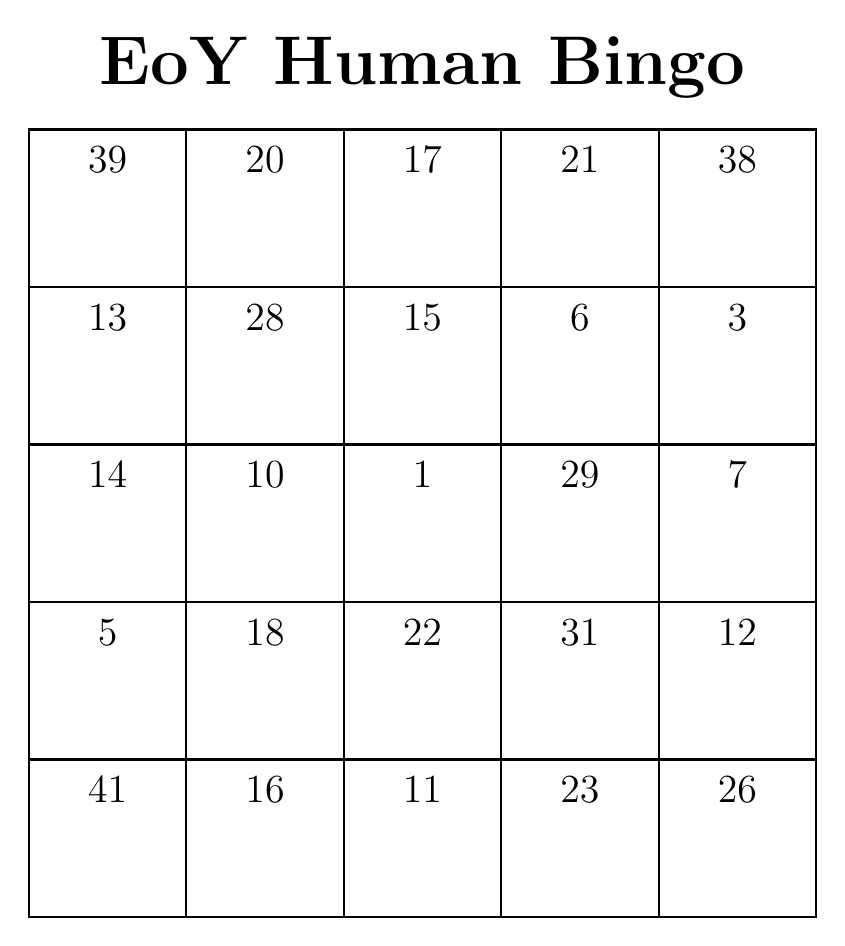
\begin{tikzpicture}
% Set the grid dimensions
\def\cellsize{2cm} % Each cell will be 2x2 cm

% Draw the grid and insert the numbers
\draw[thick] (0, 0) rectangle +(2, 2);
\node[anchor=north, font=\Large, align=center] at (1.0, 1.9) {39};
\draw[thick] (2, 0) rectangle +(2, 2);
\node[anchor=north, font=\Large, align=center] at (3.0, 1.9) {20};
\draw[thick] (4, 0) rectangle +(2, 2);
\node[anchor=north, font=\Large, align=center] at (5.0, 1.9) {17};
\draw[thick] (6, 0) rectangle +(2, 2);
\node[anchor=north, font=\Large, align=center] at (7.0, 1.9) {21};
\draw[thick] (8, 0) rectangle +(2, 2);
\node[anchor=north, font=\Large, align=center] at (9.0, 1.9) {38};
\draw[thick] (0, -2) rectangle +(2, 2);
\node[anchor=north, font=\Large, align=center] at (1.0, -0.1) {13};
\draw[thick] (2, -2) rectangle +(2, 2);
\node[anchor=north, font=\Large, align=center] at (3.0, -0.1) {28};
\draw[thick] (4, -2) rectangle +(2, 2);
\node[anchor=north, font=\Large, align=center] at (5.0, -0.1) {15};
\draw[thick] (6, -2) rectangle +(2, 2);
\node[anchor=north, font=\Large, align=center] at (7.0, -0.1) {6};
\draw[thick] (8, -2) rectangle +(2, 2);
\node[anchor=north, font=\Large, align=center] at (9.0, -0.1) {3};
\draw[thick] (0, -4) rectangle +(2, 2);
\node[anchor=north, font=\Large, align=center] at (1.0, -2.1) {14};
\draw[thick] (2, -4) rectangle +(2, 2);
\node[anchor=north, font=\Large, align=center] at (3.0, -2.1) {10};
\draw[thick] (4, -4) rectangle +(2, 2);
\node[anchor=north, font=\Large, align=center] at (5.0, -2.1) {1};
\draw[thick] (6, -4) rectangle +(2, 2);
\node[anchor=north, font=\Large, align=center] at (7.0, -2.1) {29};
\draw[thick] (8, -4) rectangle +(2, 2);
\node[anchor=north, font=\Large, align=center] at (9.0, -2.1) {7};
\draw[thick] (0, -6) rectangle +(2, 2);
\node[anchor=north, font=\Large, align=center] at (1.0, -4.1) {5};
\draw[thick] (2, -6) rectangle +(2, 2);
\node[anchor=north, font=\Large, align=center] at (3.0, -4.1) {18};
\draw[thick] (4, -6) rectangle +(2, 2);
\node[anchor=north, font=\Large, align=center] at (5.0, -4.1) {22};
\draw[thick] (6, -6) rectangle +(2, 2);
\node[anchor=north, font=\Large, align=center] at (7.0, -4.1) {31};
\draw[thick] (8, -6) rectangle +(2, 2);
\node[anchor=north, font=\Large, align=center] at (9.0, -4.1) {12};
\draw[thick] (0, -8) rectangle +(2, 2);
\node[anchor=north, font=\Large, align=center] at (1.0, -6.1) {41};
\draw[thick] (2, -8) rectangle +(2, 2);
\node[anchor=north, font=\Large, align=center] at (3.0, -6.1) {16};
\draw[thick] (4, -8) rectangle +(2, 2);
\node[anchor=north, font=\Large, align=center] at (5.0, -6.1) {11};
\draw[thick] (6, -8) rectangle +(2, 2);
\node[anchor=north, font=\Large, align=center] at (7.0, -6.1) {23};
\draw[thick] (8, -8) rectangle +(2, 2);
\node[anchor=north, font=\Large, align=center] at (9.0, -6.1) {26};
\node[anchor=north, font = \Huge] at (5.0, 3.3){\textbf{EoY Human Bingo}};
\end{tikzpicture}
\end{center}
\newpage\begin{center}
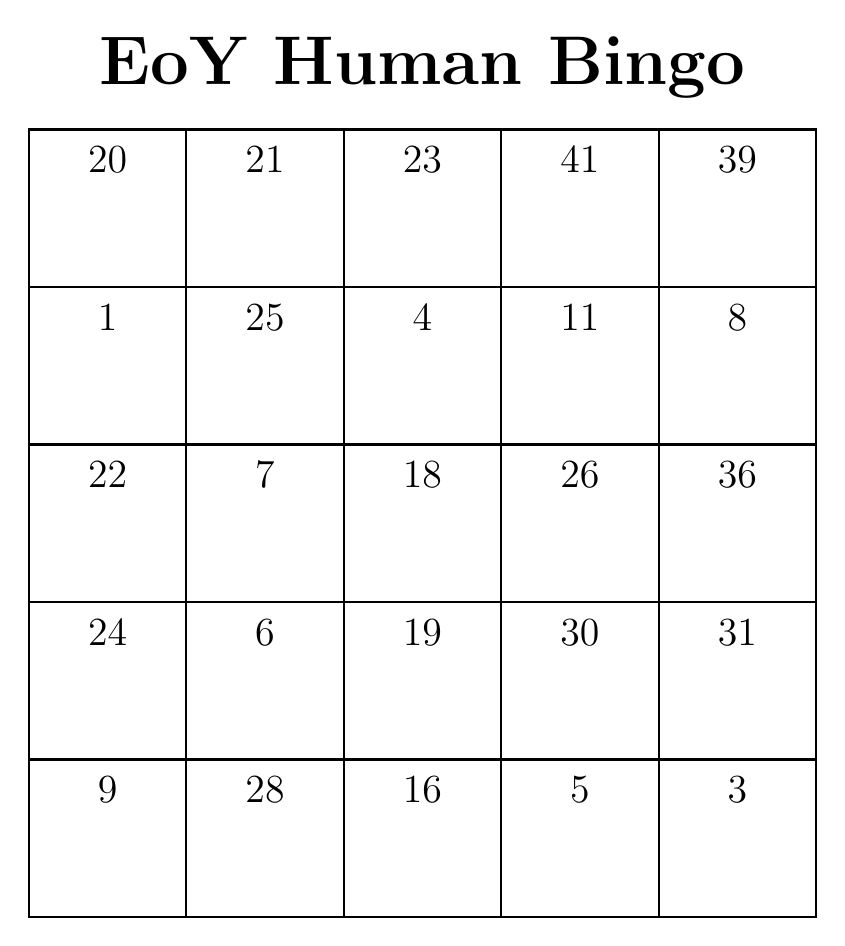
\begin{tikzpicture}
% Set the grid dimensions
\def\cellsize{2cm} % Each cell will be 2x2 cm

% Draw the grid and insert the numbers
\draw[thick] (0, 0) rectangle +(2, 2);
\node[anchor=north, font=\Large, align=center] at (1.0, 1.9) {20};
\draw[thick] (2, 0) rectangle +(2, 2);
\node[anchor=north, font=\Large, align=center] at (3.0, 1.9) {21};
\draw[thick] (4, 0) rectangle +(2, 2);
\node[anchor=north, font=\Large, align=center] at (5.0, 1.9) {23};
\draw[thick] (6, 0) rectangle +(2, 2);
\node[anchor=north, font=\Large, align=center] at (7.0, 1.9) {41};
\draw[thick] (8, 0) rectangle +(2, 2);
\node[anchor=north, font=\Large, align=center] at (9.0, 1.9) {39};
\draw[thick] (0, -2) rectangle +(2, 2);
\node[anchor=north, font=\Large, align=center] at (1.0, -0.1) {1};
\draw[thick] (2, -2) rectangle +(2, 2);
\node[anchor=north, font=\Large, align=center] at (3.0, -0.1) {25};
\draw[thick] (4, -2) rectangle +(2, 2);
\node[anchor=north, font=\Large, align=center] at (5.0, -0.1) {4};
\draw[thick] (6, -2) rectangle +(2, 2);
\node[anchor=north, font=\Large, align=center] at (7.0, -0.1) {11};
\draw[thick] (8, -2) rectangle +(2, 2);
\node[anchor=north, font=\Large, align=center] at (9.0, -0.1) {8};
\draw[thick] (0, -4) rectangle +(2, 2);
\node[anchor=north, font=\Large, align=center] at (1.0, -2.1) {22};
\draw[thick] (2, -4) rectangle +(2, 2);
\node[anchor=north, font=\Large, align=center] at (3.0, -2.1) {7};
\draw[thick] (4, -4) rectangle +(2, 2);
\node[anchor=north, font=\Large, align=center] at (5.0, -2.1) {18};
\draw[thick] (6, -4) rectangle +(2, 2);
\node[anchor=north, font=\Large, align=center] at (7.0, -2.1) {26};
\draw[thick] (8, -4) rectangle +(2, 2);
\node[anchor=north, font=\Large, align=center] at (9.0, -2.1) {36};
\draw[thick] (0, -6) rectangle +(2, 2);
\node[anchor=north, font=\Large, align=center] at (1.0, -4.1) {24};
\draw[thick] (2, -6) rectangle +(2, 2);
\node[anchor=north, font=\Large, align=center] at (3.0, -4.1) {6};
\draw[thick] (4, -6) rectangle +(2, 2);
\node[anchor=north, font=\Large, align=center] at (5.0, -4.1) {19};
\draw[thick] (6, -6) rectangle +(2, 2);
\node[anchor=north, font=\Large, align=center] at (7.0, -4.1) {30};
\draw[thick] (8, -6) rectangle +(2, 2);
\node[anchor=north, font=\Large, align=center] at (9.0, -4.1) {31};
\draw[thick] (0, -8) rectangle +(2, 2);
\node[anchor=north, font=\Large, align=center] at (1.0, -6.1) {9};
\draw[thick] (2, -8) rectangle +(2, 2);
\node[anchor=north, font=\Large, align=center] at (3.0, -6.1) {28};
\draw[thick] (4, -8) rectangle +(2, 2);
\node[anchor=north, font=\Large, align=center] at (5.0, -6.1) {16};
\draw[thick] (6, -8) rectangle +(2, 2);
\node[anchor=north, font=\Large, align=center] at (7.0, -6.1) {5};
\draw[thick] (8, -8) rectangle +(2, 2);
\node[anchor=north, font=\Large, align=center] at (9.0, -6.1) {3};
\node[anchor=north, font = \Huge] at (5.0, 3.3){\textbf{EoY Human Bingo}};
\end{tikzpicture}
\end{center}
\newpage\begin{center}
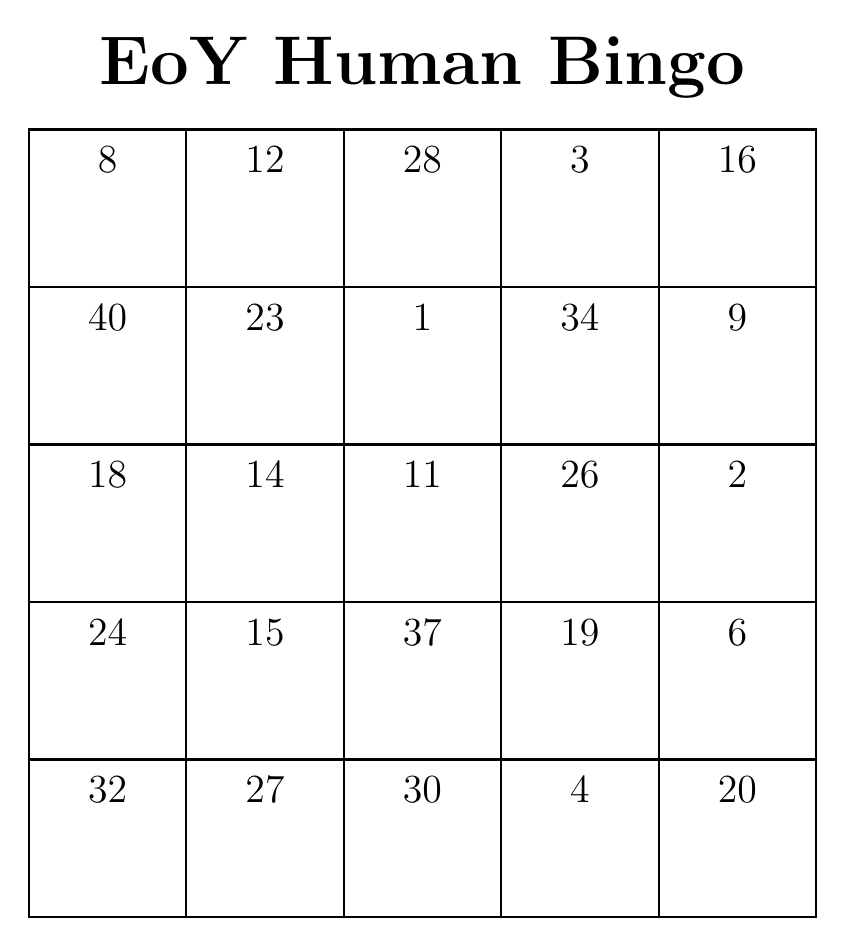
\begin{tikzpicture}
% Set the grid dimensions
\def\cellsize{2cm} % Each cell will be 2x2 cm

% Draw the grid and insert the numbers
\draw[thick] (0, 0) rectangle +(2, 2);
\node[anchor=north, font=\Large, align=center] at (1.0, 1.9) {8};
\draw[thick] (2, 0) rectangle +(2, 2);
\node[anchor=north, font=\Large, align=center] at (3.0, 1.9) {12};
\draw[thick] (4, 0) rectangle +(2, 2);
\node[anchor=north, font=\Large, align=center] at (5.0, 1.9) {28};
\draw[thick] (6, 0) rectangle +(2, 2);
\node[anchor=north, font=\Large, align=center] at (7.0, 1.9) {3};
\draw[thick] (8, 0) rectangle +(2, 2);
\node[anchor=north, font=\Large, align=center] at (9.0, 1.9) {16};
\draw[thick] (0, -2) rectangle +(2, 2);
\node[anchor=north, font=\Large, align=center] at (1.0, -0.1) {40};
\draw[thick] (2, -2) rectangle +(2, 2);
\node[anchor=north, font=\Large, align=center] at (3.0, -0.1) {23};
\draw[thick] (4, -2) rectangle +(2, 2);
\node[anchor=north, font=\Large, align=center] at (5.0, -0.1) {1};
\draw[thick] (6, -2) rectangle +(2, 2);
\node[anchor=north, font=\Large, align=center] at (7.0, -0.1) {34};
\draw[thick] (8, -2) rectangle +(2, 2);
\node[anchor=north, font=\Large, align=center] at (9.0, -0.1) {9};
\draw[thick] (0, -4) rectangle +(2, 2);
\node[anchor=north, font=\Large, align=center] at (1.0, -2.1) {18};
\draw[thick] (2, -4) rectangle +(2, 2);
\node[anchor=north, font=\Large, align=center] at (3.0, -2.1) {14};
\draw[thick] (4, -4) rectangle +(2, 2);
\node[anchor=north, font=\Large, align=center] at (5.0, -2.1) {11};
\draw[thick] (6, -4) rectangle +(2, 2);
\node[anchor=north, font=\Large, align=center] at (7.0, -2.1) {26};
\draw[thick] (8, -4) rectangle +(2, 2);
\node[anchor=north, font=\Large, align=center] at (9.0, -2.1) {2};
\draw[thick] (0, -6) rectangle +(2, 2);
\node[anchor=north, font=\Large, align=center] at (1.0, -4.1) {24};
\draw[thick] (2, -6) rectangle +(2, 2);
\node[anchor=north, font=\Large, align=center] at (3.0, -4.1) {15};
\draw[thick] (4, -6) rectangle +(2, 2);
\node[anchor=north, font=\Large, align=center] at (5.0, -4.1) {37};
\draw[thick] (6, -6) rectangle +(2, 2);
\node[anchor=north, font=\Large, align=center] at (7.0, -4.1) {19};
\draw[thick] (8, -6) rectangle +(2, 2);
\node[anchor=north, font=\Large, align=center] at (9.0, -4.1) {6};
\draw[thick] (0, -8) rectangle +(2, 2);
\node[anchor=north, font=\Large, align=center] at (1.0, -6.1) {32};
\draw[thick] (2, -8) rectangle +(2, 2);
\node[anchor=north, font=\Large, align=center] at (3.0, -6.1) {27};
\draw[thick] (4, -8) rectangle +(2, 2);
\node[anchor=north, font=\Large, align=center] at (5.0, -6.1) {30};
\draw[thick] (6, -8) rectangle +(2, 2);
\node[anchor=north, font=\Large, align=center] at (7.0, -6.1) {4};
\draw[thick] (8, -8) rectangle +(2, 2);
\node[anchor=north, font=\Large, align=center] at (9.0, -6.1) {20};
\node[anchor=north, font = \Huge] at (5.0, 3.3){\textbf{EoY Human Bingo}};
\end{tikzpicture}
\end{center}
\newpage\begin{center}
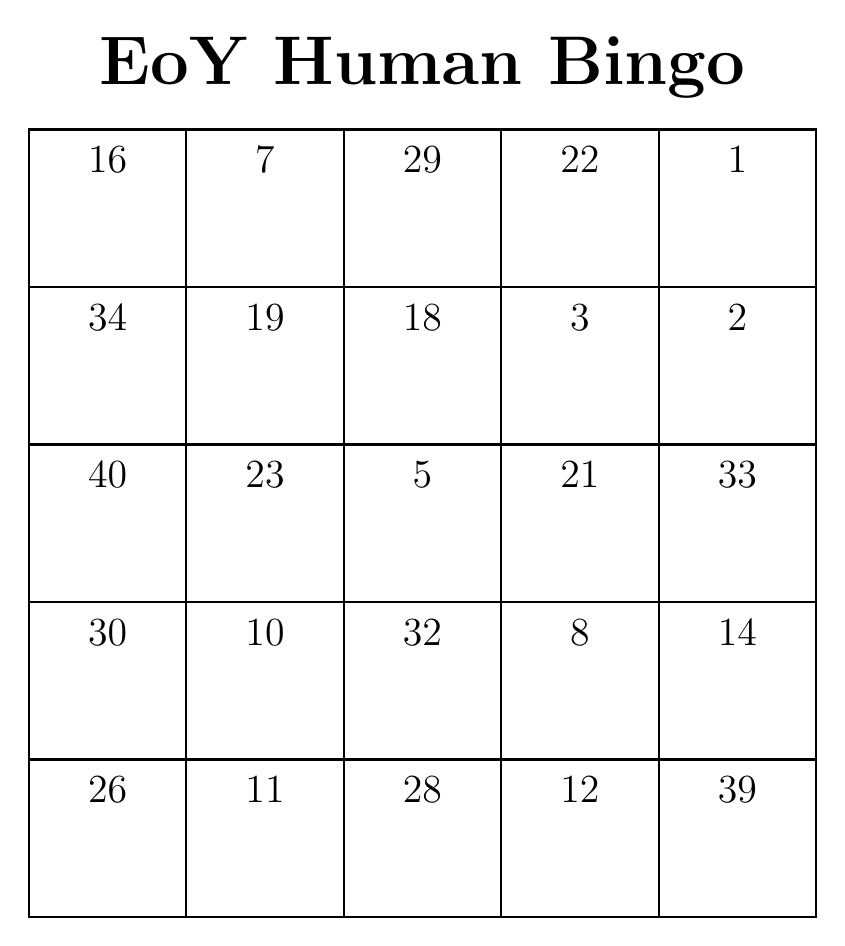
\begin{tikzpicture}
% Set the grid dimensions
\def\cellsize{2cm} % Each cell will be 2x2 cm

% Draw the grid and insert the numbers
\draw[thick] (0, 0) rectangle +(2, 2);
\node[anchor=north, font=\Large, align=center] at (1.0, 1.9) {16};
\draw[thick] (2, 0) rectangle +(2, 2);
\node[anchor=north, font=\Large, align=center] at (3.0, 1.9) {7};
\draw[thick] (4, 0) rectangle +(2, 2);
\node[anchor=north, font=\Large, align=center] at (5.0, 1.9) {29};
\draw[thick] (6, 0) rectangle +(2, 2);
\node[anchor=north, font=\Large, align=center] at (7.0, 1.9) {22};
\draw[thick] (8, 0) rectangle +(2, 2);
\node[anchor=north, font=\Large, align=center] at (9.0, 1.9) {1};
\draw[thick] (0, -2) rectangle +(2, 2);
\node[anchor=north, font=\Large, align=center] at (1.0, -0.1) {34};
\draw[thick] (2, -2) rectangle +(2, 2);
\node[anchor=north, font=\Large, align=center] at (3.0, -0.1) {19};
\draw[thick] (4, -2) rectangle +(2, 2);
\node[anchor=north, font=\Large, align=center] at (5.0, -0.1) {18};
\draw[thick] (6, -2) rectangle +(2, 2);
\node[anchor=north, font=\Large, align=center] at (7.0, -0.1) {3};
\draw[thick] (8, -2) rectangle +(2, 2);
\node[anchor=north, font=\Large, align=center] at (9.0, -0.1) {2};
\draw[thick] (0, -4) rectangle +(2, 2);
\node[anchor=north, font=\Large, align=center] at (1.0, -2.1) {40};
\draw[thick] (2, -4) rectangle +(2, 2);
\node[anchor=north, font=\Large, align=center] at (3.0, -2.1) {23};
\draw[thick] (4, -4) rectangle +(2, 2);
\node[anchor=north, font=\Large, align=center] at (5.0, -2.1) {5};
\draw[thick] (6, -4) rectangle +(2, 2);
\node[anchor=north, font=\Large, align=center] at (7.0, -2.1) {21};
\draw[thick] (8, -4) rectangle +(2, 2);
\node[anchor=north, font=\Large, align=center] at (9.0, -2.1) {33};
\draw[thick] (0, -6) rectangle +(2, 2);
\node[anchor=north, font=\Large, align=center] at (1.0, -4.1) {30};
\draw[thick] (2, -6) rectangle +(2, 2);
\node[anchor=north, font=\Large, align=center] at (3.0, -4.1) {10};
\draw[thick] (4, -6) rectangle +(2, 2);
\node[anchor=north, font=\Large, align=center] at (5.0, -4.1) {32};
\draw[thick] (6, -6) rectangle +(2, 2);
\node[anchor=north, font=\Large, align=center] at (7.0, -4.1) {8};
\draw[thick] (8, -6) rectangle +(2, 2);
\node[anchor=north, font=\Large, align=center] at (9.0, -4.1) {14};
\draw[thick] (0, -8) rectangle +(2, 2);
\node[anchor=north, font=\Large, align=center] at (1.0, -6.1) {26};
\draw[thick] (2, -8) rectangle +(2, 2);
\node[anchor=north, font=\Large, align=center] at (3.0, -6.1) {11};
\draw[thick] (4, -8) rectangle +(2, 2);
\node[anchor=north, font=\Large, align=center] at (5.0, -6.1) {28};
\draw[thick] (6, -8) rectangle +(2, 2);
\node[anchor=north, font=\Large, align=center] at (7.0, -6.1) {12};
\draw[thick] (8, -8) rectangle +(2, 2);
\node[anchor=north, font=\Large, align=center] at (9.0, -6.1) {39};
\node[anchor=north, font = \Huge] at (5.0, 3.3){\textbf{EoY Human Bingo}};
\end{tikzpicture}
\end{center}
\newpage\begin{center}
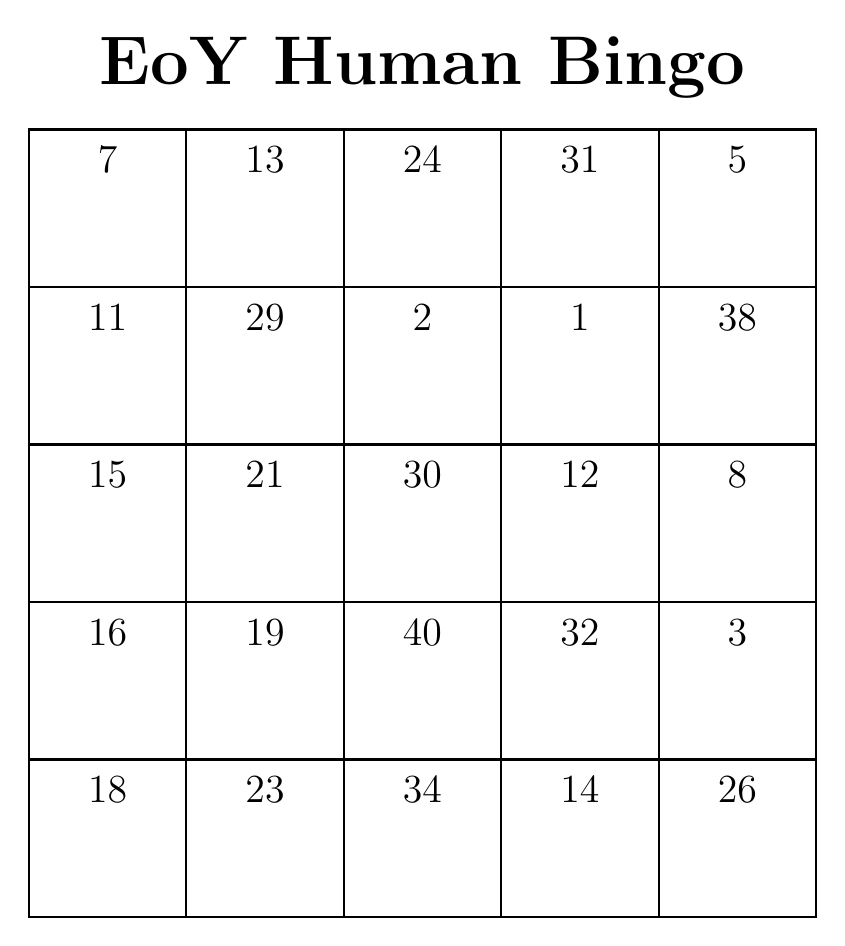
\begin{tikzpicture}
% Set the grid dimensions
\def\cellsize{2cm} % Each cell will be 2x2 cm

% Draw the grid and insert the numbers
\draw[thick] (0, 0) rectangle +(2, 2);
\node[anchor=north, font=\Large, align=center] at (1.0, 1.9) {7};
\draw[thick] (2, 0) rectangle +(2, 2);
\node[anchor=north, font=\Large, align=center] at (3.0, 1.9) {13};
\draw[thick] (4, 0) rectangle +(2, 2);
\node[anchor=north, font=\Large, align=center] at (5.0, 1.9) {24};
\draw[thick] (6, 0) rectangle +(2, 2);
\node[anchor=north, font=\Large, align=center] at (7.0, 1.9) {31};
\draw[thick] (8, 0) rectangle +(2, 2);
\node[anchor=north, font=\Large, align=center] at (9.0, 1.9) {5};
\draw[thick] (0, -2) rectangle +(2, 2);
\node[anchor=north, font=\Large, align=center] at (1.0, -0.1) {11};
\draw[thick] (2, -2) rectangle +(2, 2);
\node[anchor=north, font=\Large, align=center] at (3.0, -0.1) {29};
\draw[thick] (4, -2) rectangle +(2, 2);
\node[anchor=north, font=\Large, align=center] at (5.0, -0.1) {2};
\draw[thick] (6, -2) rectangle +(2, 2);
\node[anchor=north, font=\Large, align=center] at (7.0, -0.1) {1};
\draw[thick] (8, -2) rectangle +(2, 2);
\node[anchor=north, font=\Large, align=center] at (9.0, -0.1) {38};
\draw[thick] (0, -4) rectangle +(2, 2);
\node[anchor=north, font=\Large, align=center] at (1.0, -2.1) {15};
\draw[thick] (2, -4) rectangle +(2, 2);
\node[anchor=north, font=\Large, align=center] at (3.0, -2.1) {21};
\draw[thick] (4, -4) rectangle +(2, 2);
\node[anchor=north, font=\Large, align=center] at (5.0, -2.1) {30};
\draw[thick] (6, -4) rectangle +(2, 2);
\node[anchor=north, font=\Large, align=center] at (7.0, -2.1) {12};
\draw[thick] (8, -4) rectangle +(2, 2);
\node[anchor=north, font=\Large, align=center] at (9.0, -2.1) {8};
\draw[thick] (0, -6) rectangle +(2, 2);
\node[anchor=north, font=\Large, align=center] at (1.0, -4.1) {16};
\draw[thick] (2, -6) rectangle +(2, 2);
\node[anchor=north, font=\Large, align=center] at (3.0, -4.1) {19};
\draw[thick] (4, -6) rectangle +(2, 2);
\node[anchor=north, font=\Large, align=center] at (5.0, -4.1) {40};
\draw[thick] (6, -6) rectangle +(2, 2);
\node[anchor=north, font=\Large, align=center] at (7.0, -4.1) {32};
\draw[thick] (8, -6) rectangle +(2, 2);
\node[anchor=north, font=\Large, align=center] at (9.0, -4.1) {3};
\draw[thick] (0, -8) rectangle +(2, 2);
\node[anchor=north, font=\Large, align=center] at (1.0, -6.1) {18};
\draw[thick] (2, -8) rectangle +(2, 2);
\node[anchor=north, font=\Large, align=center] at (3.0, -6.1) {23};
\draw[thick] (4, -8) rectangle +(2, 2);
\node[anchor=north, font=\Large, align=center] at (5.0, -6.1) {34};
\draw[thick] (6, -8) rectangle +(2, 2);
\node[anchor=north, font=\Large, align=center] at (7.0, -6.1) {14};
\draw[thick] (8, -8) rectangle +(2, 2);
\node[anchor=north, font=\Large, align=center] at (9.0, -6.1) {26};
\node[anchor=north, font = \Huge] at (5.0, 3.3){\textbf{EoY Human Bingo}};
\end{tikzpicture}
\end{center}
